%%%%%%%%%%%%%%%%%%%%%%%%%%%%%%%%%%%%%%%%%%%%%%%%%%%%%%%%%%%%%%%%%%%%%%%%%%%%
%
%  ludwig.tex
%
%  Long-hand documentation for Ludwig. This file is main document
%  with style only. Content is in sections.tex
%
%  $Id$
%
%  Edinburgh Soft Matter and Statistical Physics Group and
%  Edinburgh Parallel Computing Centre
%
%  Kevin Stratford (kevin@epcc.ed.ac.uk)
%  (c) 2008 The University of Edinburgh
%
%%%%%%%%%%%%%%%%%%%%%%%%%%%%%%%%%%%%%%%%%%%%%%%%%%%%%%%%%%%%%%%%%%%%%%%%%%%%

\documentclass[11pt,twoside]{article}

\usepackage{amsmath}
\usepackage{moreverb}
\usepackage{lscape}
\usepackage{epic}
\usepackage[pdftex]{graphicx}
\usepackage{bm}
\usepackage{hyperref}
\usepackage{color}

\setlength{\hoffset}{-1in}
\setlength{\voffset}{-1in}

\setlength{\topmargin}{2cm}
\setlength{\evensidemargin}{3.1cm}
\setlength{\oddsidemargin}{3.1cm}

\setlength{\textwidth}{14.8cm}
\setlength{\textheight}{23cm}

\setlength{\parindent}{0pt}
\setlength{\parskip}{\smallskipamount}


\newcommand{\inputkey}[1]{\framebox{\textbf{\texttt{#1}}}}
\newcommand{\e}[1]{\cdot10^{#1}}
\newcommand{\beq}{\begin{equation}}
\newcommand{\eeq}{\end{equation}}
\newcommand{\beqa}{\begin{eqnarray}}
\newcommand{\eeqa}{\end{eqnarray}}
\newcommand{\com}[1]{\textcolor{red}{#1}}
\newcommand{\cur}[1]{{\textit{#1}}}

\begin{document}

\setcounter{page}{1}

\tableofcontents

\newpage

\setcounter{page}{1}

%%%%%%%%%%%%%%%%%%%%%%%%%%%%%%%%%%%%%%%%%%%%%%%%%%%%%%%%%%%%%%%%%%%%%%%%%%%%%%
%
%  intro.tex
%
%  Contains introduction and quick start for users.
%
%  Edinburgh Soft Matter and Statistical Physics Group and
%  Edinburgh Parallel Computing Centre
%
%  (c) 2016-2018 The University of Edinburgh
%
%%%%%%%%%%%%%%%%%%%%%%%%%%%%%%%%%%%%%%%%%%%%%%%%%%%%%%%%%%%%%%%%%%%%%%%%%%%%%%

\section{Introduction}

\subsection{Overview}

This introduction provides a brief overview of what the \textit{Ludwig} code
does, how to obtain and build it, and how to run a sample problem.
It is assumed that the reader has at least a general knowledge
of Navier-Stokes hydrodynamics, complex fluids, and to some
extent statistical physics. This knowledge will be required to make sense
of the input and output involved in using the code. Those wanting
to work on or develop the code itself will need knowledge of ANSI C,
and perhaps message passing and CUDA. We assume the reader is using
a Unix-based system.

\subsubsection{Purpose of the code}

The \textit{Ludwig} code has been developed over a number of
years to address specific problems in complex fluids. The underlying
hydrodynamic model is based on the lattice Boltzmann equation
(LBE, or just `LB'). This itself may be used to study simple
(Newtonian) fluids in a number of different scenarios, including porous
media and particle suspensions. However, the
code is more generally suited to complex fluids, where a number of
options are available, among others: symmetric binary fluids and
Brazovskii smectics,
polar gels, liquid crystals, or charged fluid via a Poisson-Boltzmann
equation approach. These features are added in the framework of a
free energy approach, where specific compositional or orientational
order parameters are evolved according to the appropriate
coarse-grained dynamics, but also interact with the fluid in a
fully coupled fashion.

A number of other features are catered for is some or all situations.
These include fluctuating hydrodynamics, and appropriate fluctuating
versions of order parameter dynamics for binary solvents and liquid
crystals. Colloidal particles are available for simulation of
suspensions and dispersions, and with appropriate boundary
conditions binary mixtures, liquid crystals, and charged fluid. Shear
flow is available for fluid-only systems implemented via Lees-Edwards
sliding periodic boundaries. Not all these features play with all the
others: check the specific section of the document for details.

Broadly, the code is intended for complex fluid problems at low
Reynolds numbers, so there is no consideration of turbulence,
high Mach number flows, high density ratio flows, and so on.

\subsubsection{How the code works}

We aim to provide a robust and portable code, written in ANSI C, which
can be used to perform serial and scalable parallel simulations of
complex fluid systems based around hydrodynamics via the lattice
Boltzmann method. Time evolution of modelled quantities takes
place on a fixed regular discrete lattice. The preferred method of
dealing with the corresponding order parameter equations is by
using finite difference. However, for the case of a binary fluid,
a two-distribution lattice Boltzmann approach is also maintained
for historical reference.

Users control the operation of the code via a plain text input file;
output for various data are available. These data may be visualised
using appropriate third-party software (e.g., Paraview). Specific
diagnostic output may require alterations to the code.

Potential users should also note that the complex fluid simulations
enabled by \textit{Ludwig} can be time consuming, prone to instability,
and provide results which are difficult to
interpret. We make no apology for this: that's the way it is.

\subsubsection{Who should read what?}

This documentation is aimed largely at users, but includes information
that will also be relevant for developers. The documentation discusses
the underlying features of the coordinate system, hydrodynamics (LB), and
other generic features, and has a separate section for each free energy.
You will need to consult the section relevant to your problem.


\subsection{Obtaining the code}

The code is publicly available from
\texttt{http://github/ludwig-cf/ludwig/}
which provides revision control via git, issue tracking, and so on.

The current stable release is available as the master branch.


\vfill
\pagebreak

\section{Quick Start for Users}

This section provides a brief overview of compiling and running
the code, which should allow users to get off the ground.
The section assumes the code has been downloaded and you are in the
top level directory.

\subsection{Configuration}

You will need to copy one of the existing configuration files from
the \texttt{config} directory to the top level directory. This file
sets all the relevant local details for compilation and so on. For
example:
\begin{lstlisting}
$ cp config/lunix-gcc-default.mk config.mk
\end{lstlisting}
Edit the new \texttt{config.mk} file to check, or adjust, the options
as required. You will need to identify your local C compiler. The
example uses \texttt{gcc}
in serial, and \texttt{mpicc} in parallel. For MPI in particular,
local details may vary. A quick way to compile the code is via
\begin{lstlisting}
$ cd tests
$ make compile-mpi-d3q19
\end{lstlisting}
This integrates a number of separate stages which are described
indivually in the following sections. The resulting executable
will be \texttt{./src/Ludwig.exe} at the top level.

\subsubsection{targetDP}

A \texttt{targetDP} layer is required by the code in all cases. It
allows compilation for both simple CPU systems and
for a number of accelerator systems using a single source code. This
will make the appropriate choices depending what has been specified
in the top-level \texttt{config.mk} file. From the top-level directory
\begin{lstlisting}
$ cd targetDP
$ make
\end{lstlisting}
should produce the appropriate \texttt{libtarget.a} library.

\subsubsection{Serial}
\label{section:quick-serial}

First, compile the MPI stub library in the \texttt{mpi\_s}
directory. You should be able to build the library and run the
tests using, e.g.:

\begin{lstlisting}
$ make libc
gcc -Wall -I.  -c mpi_serial.c
ar -cru libmpi.a mpi_serial.o
$ make testc
gcc -Wall   mpi_tests.c -L. -lmpi
./a.out
Running mpi_s tests...
Finished mpi_s tests ok.
\end{lstlisting}

Now compile the main code in the \texttt{src} directory.
Compilation should look like:

\begin{lstlisting}
$ make serial
make serial-d3q19
make serial-model "LB=-D_D3Q19_" "LBOBJ=d3q19.o"
make lib
make libar "INC=-I. -I../mpi_s" "LIBS= -L../mpi_s -lmpi -lm"
gcc -D_D3Q19_ -Wall -O2 -I. -I../mpi_s -c model.c
gcc -D_D3Q19_ -Wall -O2 -I. -I../mpi_s -c propagation.c
...
\end{lstlisting}
which shows that the default lattice Boltzmann model is D3Q19.
Successful compilation will provide an executable \texttt{Ludwig.exe}
which is linked against the MPI stub library.

\subsubsection{Parallel}

Here, you do not need to compile the stub library. Simply compile
the main code with, e.g.,:
\begin{lstlisting}
$ make mpi
make mpi-d3q19
make mpi-model "LB=-D_D3Q19_" "LBOBJ=d3q19.o"
make libmpi
make libar "CC=mpicc"
mpicc -D_D3Q19_ -Wall -O2 -I. -c model.c
mpicc -D_D3Q19_ -Wall -O2 -I. -c propagation.c
...
\end{lstlisting}

Again, this should produce an executable \texttt{./Ludwig.exe}
in the current directory, this time linked against the true MPI
library.

\subsection{Running an Example}

\subsubsection{Input file}

The behaviour of \textit{Ludwig} at run time is controlled by
a plain text input file which consists of a series for key value
pairs. Each key value pair controls a parameter or parameters
within the code, for example the system size and number of time steps,
the fluid properties density and viscosity, the free energy type
and associated parameters (if required), frequency and type of
output, parallel decomposition, and so on.

For most keys, the associated property has some default value which
will be used by the code if the relevant key is not present (or
commented out) in the input file. While such default values are
chosen to be at least sensible, users need to be aware that all
necessary keys need to be considered for a given problem. However,
many keys are irrelevant for any given problem.

A significant number of example input files are available as
part of the test suite, and these can form a useful starting
point for a given type of problem. We will consider one which
uses some of the common keys.

\subsubsection{Example input}

We will consider a simple example which computes the motion of
a single spherical colloidal particle in an initially stationary
fluid of given viscosity. The velocity may be measured as a
function of time. Assume we have an executable in the \texttt{src}
directory.

Make a copy of the input file
\begin{lstlisting}
$ cp ../tests/regression/d3q19/serial-auto-c01.inp .
\end{lstlisting}

Inspection of this file will reveal the following: blank lines
and comments --- lines beginning with \texttt{\#} --- may be included,
but are ignored at run time; other lines are parsed as key value
pairs, each pair on a separate line, and with key and value separated
by one or more spaces. Values may be characters or strings, a
scalar integer or 3-vector of integers, or a scalar or 3-vector
of floating point numbers. Values which are 3-vectors are delineated
by an underscore character (not a space), e.g., \texttt{1\_2\_3},
and always correspond to a Cartesian triple $(x,y,z)$.
A given value is parsed appropriately in the context of the associated key.

So, the first few lines of the above file are:
\lstinputlisting[firstline=1, lastline= 16]
{../tests/regression/d3q19/serial-auto-c01.inp}
Here, the first key value pair \texttt{N\_cycles 40} sets the number
of time steps to 40, while the second, \texttt{size 64\_64\_64}, sets
the system size to be 64 points in each of the three coordinate
directions. The \texttt{grid} key relates to the parallel
domain decomposition as is discussed in the following
section.

\subsubsection{Run time}

The executable takes a single argument on the command line which
is the name of the input file, which should be in the same
directory as the executable. If no input file name is supplied,
the executable will look for a default \texttt{input}. If no
input file is located at all, an error to that effect will be
reported.

\textbf{Serial: }
If a serial executable is run in the normal way with the copy of the
input file as the argument the code should take around 10--20 seconds
to execute 40 steps. The fist few lines of output should look like:

\begin{lstlisting}[belowskip=0pt]
$ ./Ludwig.exe ./serial-auto-c01.inp
\end{lstlisting}
\lstinputlisting[aboveskip=0pt, firstline=1, lastline= 16]
{../tests/regression/d3q19/serial-auto-c01.log}
This output shows that the appropriate input file has been read, and
the system size set correspondingly with a number of default settings
including periodic boundary conditions. ``No free energy'' tells us we
are using a single Newtonian fluid.

Normal termination of execution is accompanied by a report
of the time take by various parts of the code, and finally by
\begin{lstlisting}
...
Ludwig finished normally.
\end{lstlisting}

\textbf{Parallel: }
The executable compiled and linked against the MPI library can
be run with the MPI launcher for the local system, often
\texttt{mpirun}. For example, a run on 8 MPI tasks produces a
similar output to that seen in the serial case, but reports
details of the local domain decomposition:
\begin{lstlisting}
$ mpirun -np 8 ./Ludwig.exe ./serial-auto-c01.inp
Welcome to Ludwig v0.1.26 (MPI version running on 8 processes)
...
System details
--------------
System size:    64 64 64
Decomposition:  2 2 2
Local domain:   32 32 32
...
\end{lstlisting}
The decomposition is controlled by the \texttt{grid} key in
the input. Here, \texttt{grid 2\_2\_2} is consistent with the
8 MPI tasks specified on the command line, and the resulting
local decomposition is 32 lattice points in each coordinate direction.
If no grid is specified in the input, or a request is
make for a grid which cannot be met (e.g., the product
of the grid dimensions does not agree with the total number
of MPI tasks available)
the code will try to determine its own decomposition as best
it can. If no valid parallel decomposition is available at all,
the code will exit with a message to that effect.

Further details of various input key value pairs are given in
relevant sections of the documentation.

\subsubsection{Output}

The standard output of the running code produces a number of
aggregate quantities which allow a broad overview of the progress
of the computation to be seen by the user. These include, where
relevant, global statistics related to fluid density and momentum,
the integrated free energy, particle-related quantities, and so on.
The frequency of this information can be adjusted from the input
file (see, e.g., \texttt{freq\_statistics}).

Output for lattice-based quantities (for example, the velocity field
$u(\mathbf{r}; t)$) is via external file. This output is in serial
or in parallel according to how the model is run, and may be in
either ASCII or raw binary format as required. Output files are produced
with time step encoded in the file, and an extension which describes the
parallel output decomposition. Further, each quantity output in this way
is accompanied by a metadata description with \texttt{meta} extension.
For example, the two output files
\begin{lstlisting}
bash-3.2$ ls dist*
dist-00000020.001-001   dist.001-001.meta
\end{lstlisting}
contain the LB distributions for time step 20 (the file is 1 of a total
number of 1 in parallel), and the plain text metadata description,
respectively.

To ensure output for based-based quantities is in the correct order for
analysis, post-processing
may be required (always if the code is run in parallel). This uses a utility
provided for the purpose which required both the data and the metadata
description to recombine the parallel output. This utility is described
ELSEWHERE.

Output for colloidal particle data is again to file with a name encoding
the time step and parallel decomposition of the output. For example,
\begin{lstlisting}
bash-3.2$ ls config*
config.cds00000020.001-001
\end{lstlisting}
contains particle data for time step 20 in a format described in
Section~\ref{section-examples}.
These data may be requested in ASCII or raw binary format.

\subsubsection{Errors and run time failures}

The code attempts to provide meaningful diagnostic error messages
for common problems. Such errors include missing or incorrectly
formatted input files, inconsistent input values, and unacceptable
feature combinations. The code should also detect other run time
problems such as insufficient memory and errors writing output
files. These errors will result in termination.

Instability in the computation will often be manifested by numerically
absurd values in the statistical output (ultimately \texttt{NaN} in
many cases). Instability may or may not result in termination, depending
on the problem. Such instability is very often related to poor parameter
choices, of which there can be many combinations. Check the
relevant section of the documentation for advice on reasonable starting
parameters for different problems.


\subsection{Note on Units}

All computation in \textit{Ludwig} is undertaken in ``lattice
units,'' fundamentally related to the underlying LB fluid model
which expects discrete model space and time steps
$\Delta x = \Delta t = 1$. The natural way to approach problems
is then to ensure that appropriate dimensionless quantities are
reasonable. However, ``reasonable'' may not equate to ``matching
experimental values''. For example, typical flows in colloidal
suspensions my exhibit Reynolds numbers as low as $O(10^{-6})$
to $O(10^{-8})$.
Matching such a value in a computation may imply an impractically
small time step; a solution is to let the Reynolds number rise
artificially with the constraint that it remains small compared to $O(1)$.
Further discussion of the issue of units is provided in, e.g.,
\cite{cates_scaling}. Again, consult the relevant section of the documentation
for comments on specific problems.


\vfill
\pagebreak


\clearpage
\vfill\pagebreak
\section{Code Design}

\subsection{Some Comments}

In designing a code in C the main object of which is to do high
performance computing, there are some inevitable tensions with
software engineering best-practice. In particular, complete
encapsulation of data in the spirit of using abstract data types
tends to cause problems of performance.

For example, encapsulation of the lattice Boltzmann distribution
$f_i$, together with appropriate ``get'' and ``set'' functions for
access when approapriate, is possible. There could then be a
complete separation of interface and implementation of the
distribution (other than that each individual $f_i$ is represented
by a \texttt{double}). However, experience suggests that
this imposes severe impediment to optimisation and hence
unacceptable performance degradation.

Schemes do exist by which one can approximate the object
oriented programming style in C, and so achieve a separation
of interface and implementation. However, this tends to put
a heavy burden on the use of \texttt{void} pointers, itself
a recipe for possible disaster. A truly object-oriented
language such as Java would be preferable.

So, for the time being, some relaxation of encapsulation is required.
Exposing a pointer to the distributions which allows them to be accessed
directly where required. This can be done merely by declaring the
necessary variables \texttt{extern}. In practice, such deviations
from encapsulation can be minimised in the lattice sector of the
code. In particlar, \texttt{extern} declarations should not be
required in \texttt{main()}, i.e., it should be able to write a
new application without worrying about details of implementation.

\subsubsection{Objects}

Somewhat more difficult is the part of the code involving
colloids, which would really favour a truly object-oriented
approach.

\subsubsection{Serial and parallel}

The design decission has been taken to support execution of the
code in both serial and parallel. The default compilation
assumes that a serial executable is required, while  MPI code
is introduced via C-preprocessor directives (\texttt{-D\_MPI\_}).


There is no shared memory inplementation at this time.


\subsection{Structural Components: \texttt{MPI\_COMM\_WORLD}}


\subsection{Coordinate System: \texttt{MPI\_CARTESIAN\_COMMUNICATOR}}


\begin{figure}
\begin{center}
%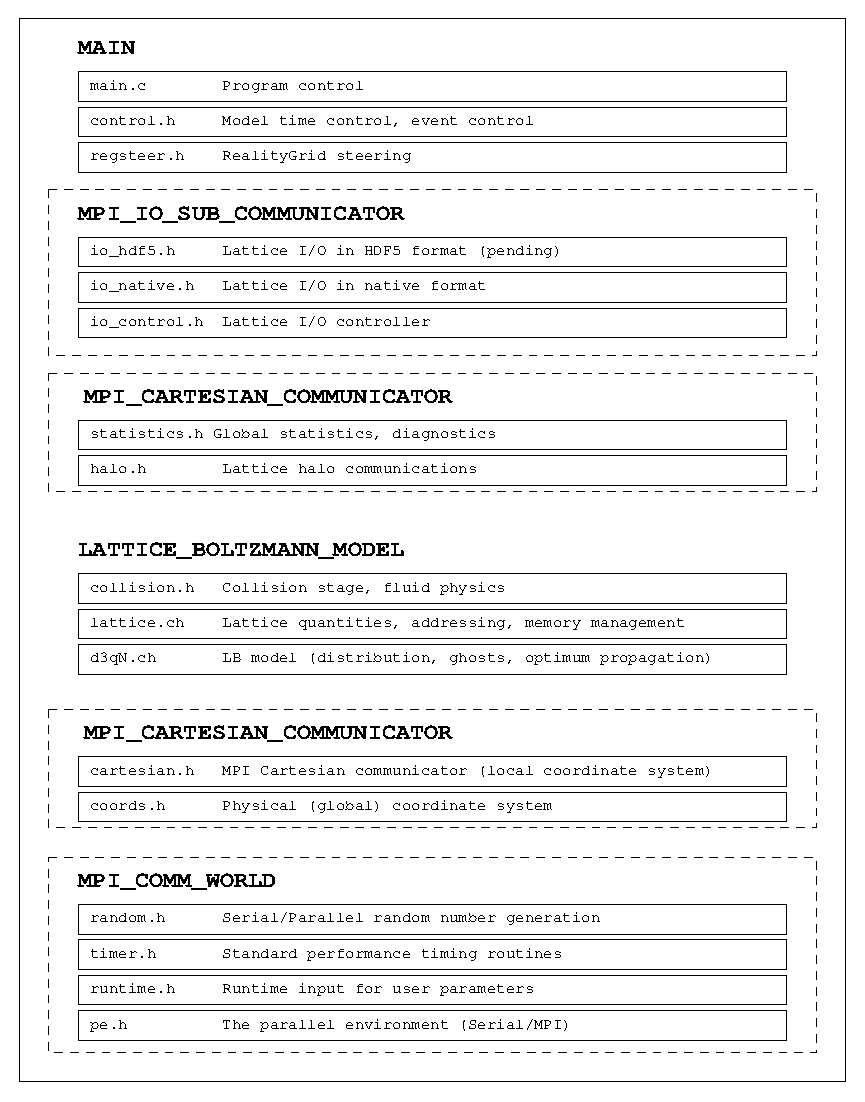
\includegraphics{xfig/sketch.eps}
\end{center}
\caption{A scheme by which different parts of the code might be
encapsulated and in such a way to allow reliable development and
testing. As this is C, will do not adopt a truly ``object'' langauge.
Broadly, different modular parts should only depend on stuff above
in the diagram. So, at the top, there is the parallel environment
where communication occurs within MPI\_COMM\_WORLD. Built on top
of this is the Cartesian Communicator responsible for halo swaps
and so forth. The LE code may have a separate Communicator again. 
(There's an argument to say the diagram should be the other way up!)}
\end{figure}

\clearpage
\vfill\pagebreak

\section{Code Implementation}

\subsection{Stuff}

\subsection{Coordinate System}

\subsubsection{The global coordinate system}

The user specifies the system size in lattice units at run time,
which sets the extent of memory which must be allocated for the
Cartesian lattice. The extent of the physical coordinate system
then reflects the lattice size directly (see Figure \ref{fig_c1}). 
Each lattice site, or node,  has coordinates corresponding to its
integer position in the system and can be thought of as being
at the centre of a control volume one lattice unit on a side.
This means that the nominal edges of the
system are offset from the lattice sites themselves by half a
lattice unit in each direction.


\begin{figure}[h]
\begin{center}
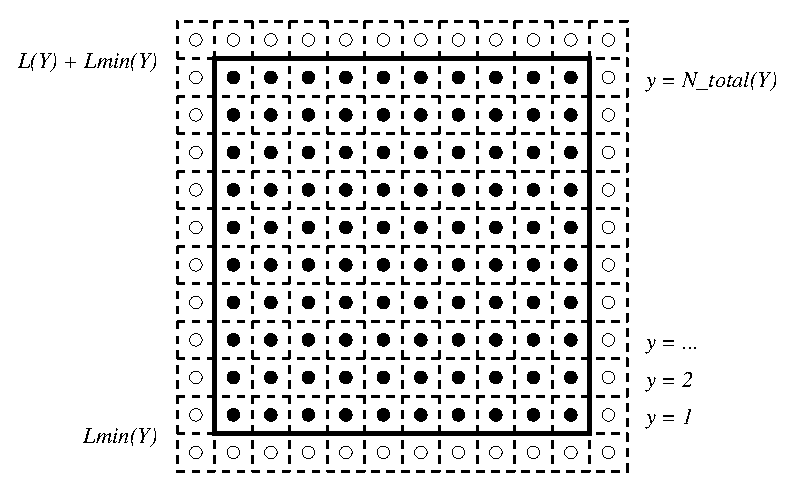
\includegraphics{xfig/fig_c1.eps}
\end{center}
\caption{The global Cartesian coordinate system reflects the choice
of lattice size; lattices sites are located at
$x=1, \ldots, x = N_{total}$ and so on in each coordinate direction
(the Figure only shows the labels in the $y-$direction for simplicity).
In the Figure, the lattice sites in the domain proper are the full
circles; halo sites, which are used to effect periodic boundary
conditions, are included as open cirles}
\label{fig_c1}
\end{figure}

For particles, the centres of which can move continuously across the
lattice, the extents of the global coordinate system are then
$L_{min} < x < L + L_{min}$ and so on.

\subsubsection{Addressing the lattice: the local coordinate system}


\subsection{Solid walls}

General solid objects which are fixed for the duration of
the simulation, such as porous media, can be defined
by assigning solid/fluid status to each lattice node. 
The links required between solid and fluid nodes can
then be identified for the given model.

\textit{Comment.} In general, a solid object will not
affect the periodic nature of the simulation. A general
solid object cannot move, i.e., the boundary velocity
must be zero.

\textit{Special case.} In the case where the solid object
represents a flat boundary wall at the edge of the system
in one or more directions, the periodicity is broken in
the corresponding directions.



%%%%%%%%%%%%%%%%%%%%%%%%%%%%%%%%%%%%%%%%%%%%%%%%%%%%%%%%%%%%%%%%%%%%%%%%%%%%%
% LE Implementation
%%%%%%%%%%%%%%%%%%%%%%%%%%%%%%%%%%%%%%%%%%%%%%%%%%%%%%%%%%%%%%%%%%%%%%%%%%%%%

\subsection{Lees Edwards Sliding Period Boundary Conditions}

\subsubsection{The LE module}

\subsubsection{Distributions crossing the LE planes}

With the planes conceptually half-way between lattice sites, the
propagation moves some of the distributions (namely, those with
$c_x = \pm1$) between different sliding blocks. While the collision
stage is unaffected, action must be taken to adjust these
distributions when the LE boundary conditions are active. This
is done in a two-stage process described by Adhikari \textit{et al.}
\cite{adhikari_desplat}, implemented between the collision and
propagation.

\textbf{a. Reprojection} The post-collision distributions with
$c_x = \pm 1$ at sites adjacent to a boundary are modified to
take account of the velocity jump $\pm u^{LE}_y$ between the sliding
blocks. In terms of the hydrodynamic moments we have:
\begin{eqnarray}
\rho &\rightarrow& \rho', \\
\rho u_\alpha &\rightarrow& (\rho u_\alpha)' \pm \rho' u^{LE}_\alpha, \\
S_{\alpha\beta} &\rightarrow&
S'_{\alpha\beta} \pm (\rho u_\alpha)' u^{LE}_\beta
\pm (\rho u_\beta)' u^{LE}_\alpha + \rho' u^{LE}_\alpha u^{LE}_\beta.
\end{eqnarray}
If we work with the changes to the moemnts, then the density is
unaffected $\delta\rho =  0$, the velocity is changed by
$\delta u_\alpha = \pm u^{LE}_\alpha$, with an analogous expression for
the change in the stress
\begin{equation}
\delta S_{\alpha\beta} =
\pm (\rho u_\alpha)' u^{LE}_\beta
\pm (\rho u_\beta)' u^{LE}_\alpha + \rho' u^{LE}_\alpha u^{LE}_\beta.
\end{equation}
We can then work out the change in the distributions by reprojecting
via Eq.\ref{eq:}, i.e.,
\begin{equation}
f_i \rightarrow f_i' + w_i \Bigg(
\frac{\rho \delta u_\alpha c_{i\alpha}}{c_s^2} +
\frac{\delta S_{\alpha\beta}Q_{i\alpha\beta}}{2c_s^4} \Bigg).
\end{equation}
A similar set of expressions are given for the order parameter
distributions in Adhikari \textit{et al.} \cite{adhikari_desplat}.

\textbf{b. Interpolation of reprojected distributions}
As the sliding blocks are displaced continuously with
$\delta y = u_y^{LE}t$, which is not in general a whole number of
lattice spacings, an interpolation is also required before
propagation can take place. Consider the situation (Fig.~\ref{fig_le2}) from
a stationary frame where the frame above has translated a small
distance to the right ($\delta y < \Delta y$). In the stationary frame
we must interpolate the ditributions with $c_x = 1$ to a
`departure point' from which the propagation will move the
distribution exactly to the appropriate lattice site in the moving
frame. Schemeatically,
\begin{equation}
f_i'(x, y + \delta y, z) = 
 (1 - \delta y) f_i^\star(x, y, z) +
\delta y f_i^\star(x, y + \Delta y, z),
\end{equation}
where $f_i'$ here represents the interpolated value and $f_i^\star$
is the reprojected post-collision quantity.

In the case where the displacement $\delta y > 1$, the relevant
lattice sites involved in the interpolation are displaced to the right
by the integral part of $\delta y$, while the relative weight given to
the two sites involves
the fractional part of $\delta y$. To take account of the periodic
boundary conditions
in the $y$-direction, all displacements are modulo $L_y$.


\begin{figure}[h]
\begin{center}
%\includegraphics{xfig/fig_le2.eps}
\end{center}
\caption{Schematic diagram showing interpolation of distributions in the
stationary plane (below) in preparation for propagation into the moving
frame (above). For a small displacement $\delta y = u^{LE} t$, the
interpolation takes place between lattice sites in the stationary frame
(green, left). Propogation from the interpolated positions (red) can
then take place into the moving frame (right).}
\label{fig_le2}
\end{figure}


In parallel, exactly the same calculation is undertaken. However,
communication is required to take account of the processor
decomposition in the $y$-direction. This requires the identification
of the two processes which hold the relevant information as a function
of displacement. 

Note that the interpolated values are stored in the appropriate lattice
site in the rest frame that ensures the normal propagation stage moves all
distributions to the correct destination in memory.

\subsubsection{Order parameter gradients}

When the order parameter gradient is computed at a given point
near the LE boundaries, the stencil may extend out of the stationary
frame. The process of interpolation is slightly different to that
for the distributions.

Here, we need to interpolate values in the moving frame to the position
which is seen by the rest frame. Figure~\ref{fig_le3} shows a five-point
stencil to calculate the gradient at the central point $(x,y,z)$ in the
rest frame. An interpolation of the $\phi$-field of the form
\begin{equation}
\phi'(x + \Delta x, y - \delta y, z) =
\delta y \phi(x + \Delta x,  y - \Delta y, z) + 
(1 - \delta y) \phi(x + \Delta x, y, z)
\end{equation}
must then take place. In practice, the interpolated values are stored
in the offset buffer. As the gradient calculation requires $\phi$
values in the halo regions, interpolated values for the buffer halo
region are also required.

\begin{figure}[h]
\begin{center}
%\includegraphics{xfig/fig_le3.eps}
\end{center}
\caption{Schematic diagram showing a five-point stencil to compute a
gradient at the central point in the stationary frame. The upper point
of the stencil is in the moving frame and so must be interpolated to
the correct position (red sites).}
\label{fig_le3}
\end{figure}

In parallel, the interpolation requires data from at most two adjacent
processes in the along-plane $y-$direction as long as the $\phi$ halo
regions are up-to-date. The rank of the processes involved is
determined by the displacement $\delta y$ as a function of time.


\subsubsection{Velocities and finite-difference fluxes}

For the finite-difference implementation, the velocity field at
the cell boundaries is required. At the planes, this means an
interpolation which takes the same form as that for
$\phi$ is needed.

In computing the advective fluxes between cells, we must then
allow for the presence of the planes. This is done by computing
separately the 'east' and 'west' face fluxes in the $x$-direction
(the flux that crosses the plane). Away from the planes, face-flux
uniqueness $f_{ijk}^e = f_{i+1jk}^w$ ensures conservation of order
parameter. However, at the planes, the non-linear conbination of
velocity field and order parameter field does not in general give
rise to consistent fluxes. In order to restore conservation, we
reconcile east and west face fluxes at the plane by taking an
average
\begin{eqnarray}
f_{ijk}^{e\star}&=&{\textstyle\frac{1}{2}}(f_{ijk}^e + f_{i+1j'k}^w),\quad 
f_{i+1j'k}^w  = \delta y f_{i+1 j-1 k}^w + (1 - \delta y) f_{i+1jk}^w,\\
f_{i+1 j k}^{w\star} &=& {\textstyle\frac{1}{2}}(f_{ij'k}^e + f_{i+1jk}^w),\quad
f_{ij'k}^e = (1 - \delta y) f_{ijk}^e + \delta y f_{ij+1k}^e.
\end{eqnarray}
In this way, we average the east face flux in the rest frame $f_{ijk}^e$
with the interpolated value of the west face flux in the moving frame
$f_{i+1j'k}^w$, and vice-versa. One can then easily show that when
integrated over the length of the plane, the average fluxes are
consistent, i.e.,
\begin{equation}
\sum_j (f_{ijk}^{e\star} - f_{i+1jk}^{w\star}) = 0 \quad\forall k,
\end{equation}
thus ensuring order parameter conservation.

A similar correction is required when computing the force on the fluid
directly via the divergence of the thermodynamic stress
$F_\alpha = \nabla_\beta P_{\alpha\beta}^{th}$. This is implementated
by computing fluxes of momentum at cell faces in each direction, and
then taking the divergence to compute the force. At the planes, an
averaging procedure is again used to ensure conservation of momentum.

%%%%%%%%%%%%%%%%%%%%%%%%%%%%%%%%%%%%%%%%%%%%%%%%%%%%%%%%%%%%%%%%%%%%%%%%%%%%%
% End LE implementation
%%%%%%%%%%%%%%%%%%%%%%%%%%%%%%%%%%%%%%%%%%%%%%%%%%%%%%%%%%%%%%%%%%%%%%%%%%%%%


\clearpage
\vfill\pagebreak

\section{Code Interface}

\subsection{The Parallel Environment}

\texttt{\#include ``pe.h''}

As the code is to be available in both serial and parallel versions,
it is desirable to abstract the basic environment to some extent.
The parallel environment is intended to support MPI communication
within \texttt{MPI\_COMM\_WORLD}, or fall back to a minimally
consistent picture in serial (i.e., rank zero is the single process).

\texttt{void pe\_init(int argc, char ** argv)}\\
Responsible for initialisation of MPI, and hence must be first
execuatable statement. The arguments are those to \texttt{main}
which will be passed through to \texttt{MPI\_Init()}.

\texttt{int pe\_rank(void)}\\
Returns the process rank in \texttt{MPI\_COMM\_WORLD}, or 0 in
serial.

\texttt{int pe\_size(void)}\\
Returns the number of processes in \texttt{MPI\_COMM\_WORLD}, or
1 in serial.

\texttt{void pe\_finalise(void)}\\
Responsible for \texttt{MPI\_Finalize()}, and must be the last
executable statement.

\texttt{void info(const char * fmt, ...)}\\
Behaves like \texttt{printf}, but only produces output on the
root process.

\texttt{void verbose(const char * fmt, ...)}\\
Behaves as \texttt{printf} and reports the rank of the
calling process in \texttt{MPI\_COMM\_WORLD}.

\texttt{void fatal(const char * fmt, ...)}\\
Prints an error message and identifies
the rank of the calling process before terminating the program.


\subsection{Run Time Input}

\texttt{\#include ``runtime.h''}

The ability to set a wide range of parameters at run time is
very convenient, and is supported via an input file in which the
user specifies parameters as key value pairs. The code maintains
a list of key value pairs from which the user can retrieve the
appropriate values for given keys.


\texttt{void RUN\_read\_input\_file(const char * input\_file\_name)}\\
This reads the named input file and sets up the list of keys.

\texttt{int RUN\_get\_double\_parameter(const char *key, double * value)}\\
Set the \texttt{value} associated with \texttt{key}, if present. The number
of key matches found is returned (i.e., 0 or 1).

\texttt{int RUN\_get\_int\_parameter(const char * key, int * value)}\\
Set the \texttt{value} associated with \texttt{key}, if present. The
number of key matches is returned.

\texttt{int  RUN\_get\_string\_parameter(const char * key, char * value)}\\
Set \texttt{value} to the string assocaited with \texttt{key}, if
present. Returns the number of key matches found.

\texttt{int  RUN\_get\_int\_parameter\_vector(const char * key, int v[])}\\
If \texttt{key} is present, set the associated 3-vector of integers.
Returns the number of key matches found. 

\texttt{int  RUN\_get\_double\_parameter\_vector(const char * key,
double v[])}\\
If \texttt{key} is present, set the associated 3-vector of doubles.
Returns the number of key matches found.

\textit{Comment:} We probably need a function to report unused keys, so
the user can be alerted if a key has unexpectedly been ignored.


\subsection{Random Number Generators}

\texttt{\#include ``ran.h''}

Note that the random number generation in parallel is
decomposition dependent.

\texttt{void rand\_init(void)}\\
Responsible for initialising RNG state.

\texttt{double rand\_serial\_uniform(void)}\\
Return a single variate uniformly distributed on $[0,1]$ from
the serial generator.

\texttt{double rand\_serial\_gaussian(void)}\\
Return a single variate with Gaussian distribution about zero
and having unit variance from the serial generator.

\textit{double rand\_parallel\_uniform(void)}\\
Return a single variate uniformly distributed on $[0,1]$
from the serial generator.

\texttt{double rand\_parallel\_gaussian(void)}\\
Return a single variate with Gaussian distribution about zero
and having unit variance from the parallel generator.

\textit{Comment:} The serial generator will produce the
same sequence on any MPI process, while the parallel generator
will produce different sequences. The latter is intended for
generating, specifically, fluctuations, where the need for
decomposition-independance is questionable.



\subsection{Timers}

\texttt{\#include ``timer.h''}

Performance figures require timing for different sections
of the code. The code provides a set of routines to time
standard and user-defined sections of code. Timers are
started and stopped by call to the appropriate routines.

\texttt{TIMER\_init()}\\
This initialises all the timers to zero (e.g., at the start of
the program).

\texttt{TIMER\_start(const int t\_id)}\\
Start the given timer.

\texttt{TIMER\_stop(const int t\_id)}\\
Stop the given timer.

\texttt{TIMER\_statistics(void)}\\
Prints the current state of all the active timers to standard
output on the root process in a digestible form. In serial,
the minimum, maximum, and mean time for each timer is reported
in seconds (based on the number of start/stop cycles). In
parallel, the same figures are computed on each process and the
result of the corresponding \texttt{MPI\_Reduce()} operation is
printed on the root process.

The code provides a number of timers which would time standard
parts of the code, e.g., \texttt{t\_id = TIMER\_TOTAL} for the
total execution time, and a number of spare timers for users to
use at will.


\textit{Comment:}
No intra-run variance (i.e., between time steps) is provided, as the
calculation required is considerably more complex to generalise, and
requires memory proportional to the number of time steps used.


\textit{Comment:}
Two macros, \texttt{TIMER\_START()} and \texttt{TIMER\_STOP()} are
provided to insert calls to the above functions for optional timing
of performance-sensitive regions
of the code in conjunction with the preprocessor flag
\texttt{-D\_TIMING\_MACRO\_ON\_}.


\subsection{Model Time Control}

This provides time step control, event frequency (?)

\texttt{void init\_control(void)}\\
Initialise time controls.

\texttt{int get\_step(void)}\\
Return the current model time step.

\texttt{int next\_step(void)}\\
Increments the current time step. Returns number of steps left
to run (i.e., 0 when finished).



\subsection{Coordinate System}

\texttt{\#include ``coords.h''}

A three-dimensional Cartesian coordinate system is used throughout,
with the exact system size usually chosen by the user at run time.
The symbolic constants \texttt{X}, \texttt{Y}, and \texttt{Z} are
used to identify the coordinate directions.

This also provides access to the MPI Cartesian Communicator which
is responsible for most communication in the model.

\texttt{int N\_total(const int dim)}\\
Returns the total number of lattice sites in the given Cartesian direction.

\texttt{double L(const int dim)}\\
Returns the length of the system in the given Cartesian direction
(which is the same as the number of lattice sites).

\texttt{double Lmin(const int dim)}\\
Returns coordinate position of left-hand edge of system in given
Cartesian direction.

\texttt{int is\_periodic(const int dim)}\\
Returns 1 if given Cartesian direction is periodic, else 0.

\texttt{void cart\_init(void)}\\
Responsible for setting up the Cartesian decomposition.

\texttt{int cart\_rank(void)}\\
Returns rank in the Cartesian communicator.

\texttt{MPI\_Comm cart\_comm(void)}\\
Returns the MPI Communicator handle for the Cartesian communicator.

\texttt{int cart\_size(const int dim)}\\
Returns the size of the Cartesian communicator grid in the given
coordinate direcxtion.

\texttt{int cart\_coord(const int dim)}\\
Returns the coordinate of the current process in the Cartesian
Communicator.

\texttt{int cart\_neigh(const int dir, const int dim)}\\
Returns the rank of the neighbouring process in the
Cartesian communicator.


\subsection{Colloids}

\texttt{\#include ``colloids.h''}

These functions provide the basic interface for use
of colloidal particles in the code.

\subsubsection{Colloid structure}

The basic colloid struct is defined ...
 

\subsubsection{Colloid interface}

\texttt{void colloids\_init(void)}\\
Call once for initialisation. This initialises the cell list,
so the coordinate system must be initialised via a call to
\texttt{coords\_init()} first.

\texttt{void colloids\_finish(void)}\\
Call once for finalisation. Frees all colloid-related memory.

\texttt{Colloid * allocate\_colloid(void)}\\
Returns a pointer to a newly allocated \texttt{Colloid} object
or fails gracefully.

\texttt{void free\_colloid(Colloid * p\_colloid)}\\
Deallocates all memory associated with \texttt{p\_colloid} or
fails gracefully.

\texttt{struct c\_link allocate\_boundary\_link(void)}\\
Returns a pointer to a newly allocated colloid boundary
link or fails gracefully.

\texttt{void free\_boundary\_link(struct c\_link *)}\\
Deallocates memory associated with a link or fails gracefully.

\texttt{void colloids\_memory\_report(void)}\\
The module keeps track of how much memory has been allocated in
total for colloids and boundary links. This reports the current
usage.

\texttt{get\_Ncell\_total()}\\

\texttt{get\_Ncell\_local()}\\

\texttt{Colloid * cell\_get\_colloid(int i, int j, int k)}\\
This returns a pointer to the Colloid at the head of the list at
cell list location (i, j, k) or \texttt{NULL} if there is none.

\texttt{void cell\_insert(Colloid * p\_colloid)}\\
This inserts a colloid at the head of the appropriate list
depending upon its position. This is the only way a colloid
can be added to the list.

\texttt{update\_cells(void)}\\
Performs the update of the cell list in response to updated
particle positions.

\texttt{IVector cell\_coords(FVector r)}\\




\subsection{Speculation}

\subsection{The Free Energy}

It is imagined that a single file will encapsulate all the details
of a given free energy. The interface for different choices of
free energy should be the same.


\texttt{FE\_init()}

Responsible for querying the runtime input key value pair list to
find appropriate user parameters for the free energy, or
falling back to default values.


\texttt{double FE\_get\_sigma()}

Return the surface tension. There should be a similar routine
for the interfacial thickness.

\texttt{double FE\_get\_mu(const type location)}

Return the chemical potential at the single lattice
node \texttt{location}.

\textit{Comment:} The computation of quantities such as the chemical
potential will a) affect performance and b) require halo values of
the order parameter (depending on the highest derivative
in the order parameter present). Performance here should be the
first consideration, so this needs to be handled with care.


\texttt{double pchem[ND][ND] FE\_get\_pchem(const type location)}

Return the chemical stress ${\cal P}_{\alpha\beta}$ at the
given location.

\textit{Comment:} This is an $nd \times nd$ matrix, where $nd$ is
the number of dimensions. If we are to provide explicit support for
D2Q9, \texttt{ND} will be 2, otherwise 3.


\clearpage
\vfill\pagebreak


\section{Implementation Notes}

\subsection{Serial Version}

\subsection{Efficiently Scaling Parallel Computing}

We should be thinking about the 100,000 processor regime, and
correspondingly large system sizes. To avoid embarrassment in this regime,
some issues which don't usually arise are relevant, for example:

\begin{enumerate}
\item
Large integer quantities such as
\begin{verbatim}
   N_total.x*N_total.y*N_total.z
\end{verbatim}
are likely to cause integer overflow (if default integers are 4 byte).
\item
Local data structures whose size is proportional
to the number of processors are contraindicated, e.g.,
anything like
\begin{verbatim}
p = (foo *) malloc(nprocs*sizeof(foo));
\end{verbatim}
is to be avoided. At the moment, we are in good shape on this
(apart from some functions in \texttt{misc.c}).
\item
I/O is likely become a very important issue, so may need to think
more about this.
\item
We should probably introduce a standard set of benchmarks which can
be scaled up in some systematic way, so that we can keep track of
performance over time.

\end{enumerate}




\clearpage
\vfill\pagebreak
%%%%%%%%%%%%%%%%%%%%%%%%%%%%%%%%%%%%%%%%%%%%%%%%%%%%%%%%%%%%%%%%%%%%%%%%%%%%%%
%
%  lb.tex
%
%  Section on lattice Boltzmann hydrodynamics
%
%%%%%%%%%%%%%%%%%%%%%%%%%%%%%%%%%%%%%%%%%%%%%%%%%%%%%%%%%%%%%%%%%%%%%%%%%%%%%%


\section{Lattice Boltzmann Hydrodynamics}
\label{section:lb-hydrodynamics}

We review here the lattice Boltzmann method applied to a simple
Newtonian fluid with particular emphsis on the relevant
implementation in \textit{Ludwig}.

\subsection{The Navier Stokes Equation}

We seek to solve the isothermal Navier-Stokes equations which, often
written in vector form, express mass conservation
\begin{equation}
\partial_t \rho + \boldsymbol{\nabla}.(\rho\mathbf{u}) = 0
\label{eq_mass1}
\end{equation}
and the conservation of momentum
\begin{equation}
\partial_t (\rho\mathbf{u}) + \boldsymbol{\nabla}.(\mathbf{\rho uu}) =
-\boldsymbol{\nabla}p + \eta \nabla^2 \mathbf{u}
+\zeta \boldsymbol{\nabla}(\boldsymbol{\nabla}.\mathbf{u}).
\label{eq_momentum1}
\end{equation}
Equation~\ref{eq_mass1} expresses the local rate of change of the
density $\rho(\mathbf{r}; t)$ as the divergence of the flux of
mass associated with the velocity field $\mathbf{u}(\mathbf{r}; t)$.
Equation~\ref{eq_momentum1} expresses Newton's second law for
momentum, where the terms on the right hand side represent the
force on the fluid.

For this work, it is more convenient to rewrite these equations
in tensor notation, where Cartesian coordinates ${x,y,z}$ are
represented by indices $\alpha$ and $\beta$, viz
\begin{equation}
\partial_t \rho + \nabla_\alpha (\rho u_\alpha) = 0
\end{equation}
and
\begin{equation}
\partial_t (\rho u_\alpha) + \nabla_\beta (\rho u_\alpha u_\beta)
= -\nabla_\alpha p
+  \eta \nabla_\beta (u_\alpha \nabla_\beta + \nabla_\alpha u_\beta)
+ \zeta \nabla_\alpha (\nabla_\gamma u_\gamma).
\end{equation}
Here, repeated Greek indices are understood to be summed over.
The conservation law is seem better if the forcing terms of the
right hand side are combined in the fluid stress $\Pi_{\alpha\beta}$
so that
\begin{equation}
\partial_t (\rho u_\alpha) +\nabla_\beta \Pi_{\alpha\beta} = 0.
\end{equation}
In this case the expanded expression for the stress tensor is
\begin{equation}
\Pi_{\alpha\beta} = p \delta_{\alpha\beta} + \rho u_\alpha u_\beta 
+ \eta \nabla_\alpha v_\beta + \zeta (\nabla_\gamma v_\gamma)\delta_{\alpha\beta}
\end{equation}
where $\delta_{\alpha\beta}$ is that of Kroneker. Th Navier-Stokes
equations in three dimensions have 10 degrees of freedom
(or hydrodynamic modes) being
$\rho$, three components of the mass flux $\rho u_\alpha$, and 6 independent
modes from the (symmetric) stress tensor $\Pi_{\alpha\beta}$.

\subsection{The Lattice Boltzmann Equation}

The Navier-Stokes equation may be approximated in a discrete system
by the lattice Boltzmann equation (LBE). A discrete density
distribution function $f_i(\mathbf{r}; t)$ at lattice points $\mathbf{r}$
and time $t$ evolves according to
\begin{equation}
f_i (\mathbf{r} + \mathbf{c}_i \Delta t; t + \Delta t) =
f_i (\mathbf{r}; t) + \sum_j \mathcal{L}_{ij}
\big( f_i(\mathbf{r};t) - f_i^{\mathrm{eq}}(\mathbf{r};t) \big)
\end{equation}
where $\mathbf{c}_i$ is the discrete velocity basis and $\Delta t$
is the discrete time step. The collision operator
$\mathcal{L}_{ij}$ provides the mechanism to compute a discrete
update from the non-equilibrium distribution
$f_i(\mathbf{r}; t)- f_i^\mathrm{eq}(\mathbf{r};t)$. Additional terms
may be added to this equation to represent external body forces,
thermal fluctuations, and so on. These additional terms are discussed
in the following sections.

\subsubsection{The distribution function and its moments}

In lattice Boltzmann, the density and velocity of the continuum fluid
are complemented by the  distribution function
$f_i(\mathbf{r}; t)$ defined with reference to the
discrete velocity space $c_{i\alpha}$.
It is possible to relate the hydrodynamic quantities to the distribution
function via its moments, that is
\begin{equation}
\rho(\mathbf{r};t) = \sum_i f_i(\mathbf{r};t),  \quad
\rho u_\alpha(\mathbf{r};t) = \sum_i f_i(\mathbf{r};t) c_{i\alpha},  \quad
\Pi_{\alpha\beta}(\mathbf{r};t) =
\sum_i f_i(\mathbf{r};t) c_{i\alpha} c_{i\beta}.
\label{lb-f-moments}
\end{equation}
Here, the index of the summation is over the number of discrete
velocities used as the basis, a number which will be denoted
$N_\mathrm{vel}$. For example, in three dimensions
$N_\mathrm{vel}$ is often 19 and the basis is referred to as D3Q19.

The number of moments, or modes, supported by a velocity
set is exactly $N_\mathrm{vel}$, and these can be written in general as
\begin{equation}
M^a(\mathbf{r};t) = \sum_i m_i^a f_i(\mathbf{r};t),
\end{equation}
where the $m_i$ are the eigenvectors of the collision matrix in the LBE.
For example, in the case of the density, all the 
$m_i^a = 1$ and the mode $M^a$ is the density $\rho = \sum_i f_i$. Note
that the number of modes supported by a given basis will generally excceed the
number of hydrodynamic modes; the excess modes have no direct physical
interpretation and are variously referred to as non-hydrodynamic, kinetic,
or ghost, modes.
The ghost modes take no part in bulk hydrodynamics, but may become important
in other contexts, such as thermal fluctuations and near boundaries.
The distribution function can be related to the modes
$M^a(\mathbf{r};t)$ via
\begin{equation}
f_i(\mathbf{r};t) = w_i \sum_a m_i^a N^a M^a(\mathbf{r};t).
\end{equation}
In this equation, $w_i$ are the standard LB weights appearing in the
equilibrium distribution function, while the $N^a$ are a per-mode
normalising factor uniquely determined by the orthogonality condition
\begin{equation}
N^a \sum_i w_i m_i^a m_i^b = \delta_{ab}.
\end{equation}
Writing the basis this way has the advantage that the equilibrium
distribution projects directly into the hydrodynamic modes only.
Putting it another way, we may write
\begin{equation}
f_i^\mathrm{eq} = w_i \big(\rho + \rho c_{i\alpha}u_\alpha / c_s^2
+ (c_{i\alpha} c_{i\beta} - c_s^2\delta_{\alpha\beta})
(\Pi_{\alpha\beta}^\mathrm{eq} - p\delta_{\alpha\beta})/2c_s^4 \big)
\end{equation}
where only (equilibrium) hydrodynamic quantities appear on the right hand side.

\subsubsection{Collision and relaxation times}



\subsection{Model Basis Descriptions}

\subsubsection{D2Q9}

The D2Q9 model in two dimensions consists one zero vector (0,0), four
vectors of length unity being $(\pm 1,0)$ and $(0, \pm 1)$, and four
vectors of length $\sqrt{2}$ being $(\pm 1, \pm 1)$. The eigenvectors of
the collision matrix, with associated weights and normalisers are shown
in Table~\ref{table-d2q9-spec}. In two dimensions there are six hydrodynamic
modes and a total of three kinetic modes, or ghost modes.

\begin{table}[t]
\begin{center}
\begin{tabular}{|l|r|rrrrrrrrr|r|l|}
\hline\hline
$M^a$ & $p$ & \multicolumn{9}{c|}{$m_i^a$} & $N^a$  &\\
\hline
$\rho$ & - & 1 &  1 &  1 &  1 &  1 &  1 &  1 &   1 &  1 & 1 &$\mathbf{1}$ \\
\hline
$\rho c_{ix}$ & - & 0 &  1 &  1 & 1 & 0 &  0 & -1 &  1 & -1 & 3 & $c_{ix}$ \\
\hline
$\rho c_{iy}$ & - & 0 & 1 &  0 &  -1 &  1 &  -1 & 1 & 0 & -1 & 3  &$c_{iy}$ \\
\hline
$Q_{xx}$ & 1/3 & -1 &  2 &  2 & 2 & -1 & -1 & 2 & 2 & 2 & 9/2 
& $c_{ix} c_{ix} - c_s^2$ \\
\hline
$Q_{xy}$ & - & 0 &  1 & 0 & -1 & 0 & 0 & -1 & 0 & 1 & 9 & $c_{ix} c_{iy}$ \\
\hline
$Q_{yy}$ & 1/3 & -1 &  2 & -1 & 2 & 2 & 2 & 2 & -1 & 2 & 9/2
& $c_{iy} c_{iy} - c_s^2$ \\
\hline\hline
$\chi^1$ & - &  1 & 4 & -2 & 4 & -2 & -2 & 4 & -2 & 4 & 1/4 & $\chi^1$ \\
\hline
$J_{ix}$ & - & 0 &  4 & -2 & 4 & 0 & 0 & -4 & -2 & -4 & 3/8
& $\chi^1 \rho c_{ix}$\\
\hline
$J_{iy}$ & - & 0 & 4 & 0 & -4 & -2 & 2 & 4 & 0 & -4 & 3/8
& $\chi^1 \rho c_{iy}$\\
\hline\hline
$w_i$ & 1/36 & 16 & 1 & 4 & 1 & 4 & 4 & 1 & 4 & 1 & & $w_i$\\
\hline\hline
\end{tabular}
\end{center}
\caption{Table showing the details of the basis used for the D2Q9 model
in two dimensions. The nine modes $M^a$ include six hydrodynamic modes,
one scalar kinetic mode $\chi^1$, and one vector kinetic mode $J_{i\alpha}$.
The weights in the equilibrium distribution function are $w_i$ and the
normaliser for each mode is $N^a$. The eigenvectors of the collision
matrix are the columns of the transformation matrix $m^a_i$. The prefactor
$p$ (where present) multiplies all the elements to the right in that row.}
\label{table-d2q9-spec}
\end{table}



\subsubsection{D3Q15}

The D3Q15 model in three dimensions consists of a set of vectors:
one zero vector $(0,0,0)$, six vectors of length unity being
$(\pm 1, 0, 0)$ cyclically permuted, and 8 vectors of length
$\sqrt{3}$ being $(\pm 1, \pm 1, \pm 1)$.
The eigenvalues and eigenvectors of the collision
matrix used for D3Q15 are given in Table~\ref{table-d3q15-spec}.


\begin{table}[t]
\centering
\tabcolsep=4pt
\begin{tabular}{|l|r|r|rrrrrr|rrrrrrrr|r|l|}
\hline\hline
$M^a$ & $p$ & \multicolumn{15}{c|}{$m_i^a$} & $N^a$  &\\
\hline
$\rho$ & - &
 1 &  1 &  1 &  1 &  1 &  1 &  1 &  1 &  1 &  1 &  1 &  1 &  1 &  1 &  1 &
1 &$\mathbf{1}$ \\
\hline
$\rho c_{ix}$ & - &
 0 &  1 & -1 &  0 &  0 &  0 &  0 &  1 & -1 &  1 & -1 &  1 & -1 &  1 & -1 &
3  & $c_{ix}$ \\
\hline
$\rho c_{iy}$ & - &
 0 &  0 &  0 &  1 & -1 &  0 &  0 &  1 &  1 & -1 & -1 &  1 &  1 & -1 & -1 &
3  &$c_{iy}$ \\
\hline
$\rho c_{iz}$ & - &
 0 &  0 &  0 &  0 &  0 &  1 & -1 &  1 &  1 &  1 &  1 & -1 & -1 & -1 & -1 &
3  & $c_{iz}$ \\
\hline
$Q_{xx}$ & 1/3 &
-1 &  2 &  2 & -1 & -1 & -1 & -1 &  2 &  2 &  2 &  2 &  2 &  2 &  2 &  2 &
9/2  & $c_{ix} c_{ix} - c_s^2$ \\
\hline
$Q_{yy}$ & 1/3 &
-1 & -1 & -1 &  2 &  2 & -1 & -1 &  2 &  2 &  2 &  2 &  2 &  2 &  2 &  2 &
 9/2 & $c_{iy} c_{iy} - c_s^2$ \\
\hline
$Q_{zz}$ & 1/3 &
-1 & -1 & -1 & -1 & -1 &  2 &  2 &  2 &  2 &  2 &  2 &  2 &  2 &  2 &  2 &
 9/2 & $c_{iz} c_{iz} - c_s^2$ \\
\hline
$Q_{xy}$ & - &
 0 &  0 &  0 &  0 &  0 &  0 &  0 &  1 & -1 & -1 &  1 &  1 & -1 & -1 &  1 &
9  & $c_{ix} c_{iy}$ \\
\hline
$Q_{yz}$ & - &
 0 &  0 &  0 &  0 &  0 &  0 &  0 &  1 &  1 & -1 & -1 & -1 & -1 &  1 &  1 &
9  & $c_{iy} c_{iz}$ \\
\hline
$Q_{zx}$ & - &
 0 &  0 &  0 &  0 &  0 &  0 &  0 &  1 & -1 &  1 & -1 & -1 &  1 & -1 &  1 &
9  & $c_{iz} c_{ix}$ \\
\hline\hline
$\chi^1$ & - &
-2 &  1 &  1 &  1 &  1 &  1 &  1 & -2 & -2 & -2 & -2 & -2 & -2 & -2 & -2 &
1/2 & $\chi^1$ \\
\hline
$J_{ix}$ & - &
 0 &  1 & -1 &  0 &  0 &  0 &  0 & -2 &  2 & -2 &  2 & -2 &  2 & -2 &  2 &
3/2 & $\chi^1 \rho c_{ix}$\\
\hline
$J_{iy}$ & - &
 0 &   0 &  0 &  1 & -1 &  0 &  0 & -2 & -2 &  2 &  2 & -2 & -2 &  2 &  2 &
3/2 & $\chi^1 \rho c_{iy}$\\
\hline
$J_{iz}$ & - &
 0 &   0 &  0 &  0 &  0 &  1 & -1 & -2 & -2 & -2 & -2 &  2 &  2 &  2 &  2 &
3/2 & $\chi^1 \rho c_{iz}$\\
\hline
$\chi^3$ & - &
 0 &   0 &  0 &  0 &  0 &  0 &  0 &  1 & -1 & -1 &  1 & -1 &  1 &  1 & -1 &
9 & $c_{ix} c_{iy} c_{iz}$ \\
\hline\hline
$w_i$ & 1/72 &
$16$ & 8 & 8 & 8 & 8 & 8 & 8 & 1 & 1 & 1 & 1 & 1 & 1 & 1 & 1 &
 & $w_i$\\
\hline\hline
\end{tabular}

\caption{Table showing the details of the basis used for the D3Q15 model
in three dimensions. The fifteen modes $M^a$ include two scalar kinetic
modes $\chi^1$ and $\chi^3$, and one vector kinetic mode $J_{i\alpha}$.
The weights in the equilibrium distribution are $w_i$ and the normaliser
for each mode is $N^a$. The eigenvectors of the collision matrix are the
columns of the transformation matrix $m_i^a$. The prefactor $p$ simply
multiplies all elements of $m_i^a$ in that row as a convenience.
\label{table-d3q15-spec}
}
\end{table}


\subsubsection{D3Q19}

The D3Q19 model in three dimensions is constructed with velocities:
one zero vector $(0,0,0)$, three vectors of length unity being
$(\pm 1, 0, 0)$ cyclically permuted, and twelve vectors of length
$\sqrt{2}$ being $(\pm 1, \pm 1, 0)$ cyclically permuted. The
details of the D3Q19 model are set out in Table~\ref{table-d3q19-spec}.

\begin{table}[t]
\centering
\tabcolsep=4pt
\begin{tabular}{|l||r|rrrrrr|rrrr|rrrr|rrrr|r||}
\hline\hline
$M^a$ & \multicolumn{19}{c||}{$m_i^a$} & $N^a$\\
\hline
$\rho $ & 1 &  1 &  1 &  1 &  1 &  1 &  1 & 
         1 &  1 &  1 &   1 &  1 &  1 &  1 & 1 & 1 & 1 & 1 & 1
& 1\\
\hline
$\rho c_{ix}$ & 0 &  1 &  -1 &  0 &  0 &  0 &  0 & 
         1 &  1 &  -1 &   -1 &  1 &  1 &  -1 & -1 & 0 & 0 & 0 & 0
& 3 \\
\hline
$\rho c_{iy}$ & 0 &  0 &  0 &  1 &  -1 &  0 &  0 & 
         1 &  -1 &  1 &   -1 &  0 &  0 &  0 & 0 & 1 & 1 & -1 & -1
& 3\\
\hline
$\rho c_{iz}$ & 0 &  0 &  0 &  0 &  0 &  1 &  -1 & 
         0 &  0 &  0 &   0 &  1 &  -1 &  1 & -1 & 1 & -1 & 1 & -1
& 3\\
\hline
$Q_{ixx}$ & -1 &  2 &  2 &  -1&  -1 &  -1 &  -1 & 
         2 &  2 &  2 &   2 &  2 &  2 &  2 & 2 & -1 & -1 & -1 & -1
& 9/2\\
\hline
$Q_{iyy}$ & -1 &  -1 &  -1 &  2&  2 &  -1 &  -1 & 
         2 &  2 &  2 &   2 &  -1 &  -1 &  -1 & -1 & 2 & 2 & 2 & 2
& 9/2\\
\hline
$Q_{izz}$ & -1 &  -1 &  -1 &  -1&  -1 &  2 &  2 & 
         -1 &  -1 &  -1 &   -1 &  2 &  2 & 2 & 2 & 2 & 2 & 2 & 2
& 9/2\\
\hline
$Q_{ixy}$ & 0 &  0 &  0 &  0&  0 &  0 &  0 & 
          1 &  -1 &  -1 &    1 &  0 &  0 & 0 & 0 & 0 & 0 & 0 & 0
& 9\\
\hline
$Q_{ixz}$ & 0 &  0 &  0 &  0&  0 &  0 &  0 & 
          0 &   0 &   0 &   0 &  1 & -1 & -1 & 1 & 0 & 0 & 0 & 0
& 9\\
\hline
$Q_{iyz}$ & 0 &  0 &  0 &  0&  0 &  0 &  0 & 
          0 &   0 &   0 &   0 &  0 & 0 & 0 & 0 & 1 & -1 & -1 & 1
& 9\\
\hline\hline
$\chi^1$ & 0 &  1 &  1 &  1 &  1 &  -2 &  -2 & 
         -2 &  -2 &  -2 &  -2 &  1 &  1 & 1 & 1 & 1 & 1 & 1 & 1
& 3/4\\
\hline
$\chi^1 \rho c_{ix}$ & 0 &  1 &  -1 &  0&  0 &  0 &  0 & 
         -2 &  -2 &  2 &  2 &  1 &  1 & -1 & -1 & 0 & 0 & 0 & 0
& 3/2\\
\hline
$\chi^1 \rho c_{iy}$ & 0 &  0 &  0 &  1&  -1 &  0 &  0 & 
         -2 &  2 &  -2 &  2 &  0 &  0 & 0 & 0 & 1 & 1 & -1 & -1
& 3/2\\
\hline
$\chi^1 \rho c_{iz}$ & 0 &  0 &  0 &  0&  0 &  -2 &  2 & 
         0 &  0 &  0 &  0 &  1 &  -1 & 1 & -1 & 1 & -1 & 1 & -1
& 3/2\\
\hline
$\chi^2$ & 0 &  1 &  1 &  -1&  -1 &  0 &  0 & 
         0 &  0 &  0 &  0 &  -1 &  -1 & -1 & -1 & 1 & 1 & 1 & 1
& 9/4\\
\hline
$\chi^2 \rho c_{ix}$ & 0 &  1 &  -1 &  0&  0 &  0 &  0 & 
         0 &  0 &  0 &  0 &  -1 &  -1 & 1 & 1 & 0 & 0 & 0 & 0
& 9/2\\
\hline
$\chi^2 \rho c_{iy}$ & 0 &  0 &  0 & -1&   1 &  0 &  0 & 
         0 &  0 &  0 &  0 &   0 &  0 & 0 & 0 & 1 &  1 & -1 & -1
& 9/2\\
\hline
$\chi^2 \rho c_{iz}$ & 0 &  0 &  0 &  0&  0 &  0 &  0 & 
         0 &  0 &  0 &  0 &  -1 &  1 & -1 & 1 & 1 & -1 & 1 & -1
& 9/2\\
\hline
$\chi^3$ & 1 &  -2 &  -2 &  -2&  -2 &  -2 &  -2 & 
         1 &  1 &  1 &  1 &  1 &  1 & 1 & 1 & 1 & 1 & 1 & 1
& 1/2\\
\hline\hline
$w_i$ & 12 & 2 & 2 & 2 & 2 & 2 & 2 & 
1 & 1 & 1 & 1 & 1 & 1 & 1 & 1 & 1 & 1 & 1 & 1
& \\
\hline\hline
\end{tabular}
\caption{Table showing the details of the basis used for the D3Q19 model in
three dimensions. The nineteen modes $M^a$ include ten hydrodynamic modes,
three scalr kinetic modes $\chi^1$, $\chi^2$, and $\chi^3$; there are also
two vector kinetic modes $\chi^1 \rho c_{i\alpha}$
and $\chi^2 \rho c_{i\alpha}$. The weights in the equilibrium distribution
function are $w_i$, and the normaliser for each mode is $N^a$. The
eigenvectors of the collision matrix are the columns of the transformation
matrix $m^a_i$.
\label{table-d3q19-spec}
}
\end{table}


\subsection{Fluctuating LBE}

It is possible \cite{adhikari2005} to simulate fluctuating
hydrodynamics for an isothermal fluid via the inclusion of
a fluctuating stress $\sigma_{\alpha\beta}$:
\begin{equation}
\Pi_{\alpha\beta} = p\delta_{\alpha\beta} + \rho u_\alpha u_\beta
+ \eta_{\alpha\beta\gamma\delta} \nabla_\gamma u_\delta + \sigma_{\alpha\beta}.
\end{equation}
The fluctuation-dissipation theorem relates the magnitude of this
random stress to the isothermal temperature and the viscosity.

In the LBE, this translates to the addition of a random contribution
$\xi_i$ to the distribution at the collision stage, so that
\begin{equation}
\ldots + \xi_i.
\end{equation}

For the conserved modes $\xi_i = 0$. For all the non-conserved modes,
i.e., those with dissipation, the fluctuating part may be written
\begin{equation}
\xi_i (\mathbf{r}; t) = w_i m_i^a \hat{\xi}^a (\mathbf{r}; t) N^a
\end{equation}
where $\hat{\xi}^a$ is a noise termwhich has a variance determined
by the relaxation time for given mode
\begin{equation}
\left< \hat{\xi}^a \hat{\xi}^b \right> =
\frac{\tau_a + \tau_b + 1}{\tau_a \tau_b}
\left< \delta M^a \delta M^b \right>.
\label{eq_fvar}
\end{equation}

\subsubsection{Fluctuating stress}

For the stress, the random contribution to the distributions is
\begin{equation}
\xi_i = w_i \frac{Q_{i\alpha\beta} \hat{\sigma}_{\alpha\beta}}{4c_s^2}
\end{equation}
where $\hat{\sigma}_{\alpha\beta}$ is a symmtric matrix of random
variates drawn from a Gaussian distribution with variance given
by equation~\ref{eq_fvar}. In the case that the shear and bulk
viscosities are the same, i.e., there is a single relaxation
time, then the variances of the six independent components of
the matrix are given by
\begin{equation}
\left< \hat{\sigma}_{\alpha\beta} \hat{\sigma}_{\mu\nu} \right> =
\frac{2\tau + 1}{\tau^2}
(\delta_{\alpha\mu}\delta_{\beta\nu} + \delta_{\alpha\nu} \delta_{\beta\mu}).
\end{equation}


\subsection{Hydrodynamic Boundary Conditions}

\subsubsection{Bounce-Back on Links}

A very general method for the representation of solid objects
within the LB approach was put forward by Ladd \cite{l94a, l94b}.
Solid objects (of any shape) are defined by a boundary surface
which intersects some of the velocity vectors $\mathbf{c}_i$
joining lattice nodes. Sites inside are designated solid, while
sites outside remain fluid. The correct boundary condition is
defined by identifying \textit{links} between fluid and solid
sites, which allows those elements of the distribution which would
cross the boundary at the propagation step to be ``bounced-back''
into the fluid. This bounce-back on links is an efficient method
to obtain the  correct hydrodynamic interaction between solid
and fluid.

\subsubsection{Fixed objects}

\subsubsection{Moving objects}

Colloidal particles are assumed to be spherical with a geometrical
centre $\mathbf{r}_c$, which is also the centre of mass. The
centre is allowed to move continuously across the lattice
with velocity $\mathbf{U}$; the particle has an angular velocity
$\mathbf{\Omega}$. The surface of the colloid is defined by an
input radius, $a_0$, which determines which lattice nodes are
inside or outside the colloid. (The hydrodynamic properties of
the colloid are specified by a different radius $a_h$ --- more
of this later.) The boundary links are then the set of vectors
joining lattice nodes which intersect the spherical surface
$\{\mathbf{c}_b\}$. Note that a lattice node exactly at
the solid-fluid interface is defined to be outside the colloid.

In the original approach of Ladd, fluid occupied nodes both inside
and outside the particle. The effect of the ``internal fluid'' is
known to be restricted to short time scales (compared to the
characteristic time $a_0^2/\nu$), on which the fluid inside the
particle relaxes to a solid body rotation \cite{heemels}. However,
we use fully solid particles via the approach introduced by
Nguyen and Ladd \cite{nguyen-ladd2002}.



A boundary link is defined as joining a node $\mathbf{r}$
inside the particle to one outside at $\mathbf{r} + \mathbf{c}_b \Delta t$.
If the post-collision distributions are denoted by $f^\ast$, then
the distributions must be reflected at the solid surface so that
\begin{equation}
\label{eq:colloid_bbl1}
f_{b'}(\mathbf{r}; t + \Delta t) = f_b^\ast (\mathbf{r}; t)
- \frac{2w_{c_b} \rho_0 \mathbf{u}_b.\mathbf{c}_b}{c_s^2}
\end{equation}
where the boundary link $\mathbf{c}_{b'} = -\mathbf{c}_b$.
Note that the local density at the fluid site $\rho(\mathbf{r};t)$
is replaced by
the mean fluid density $\rho_0$. in the second term on the right-hand side.
The velocity at the boundary is
\begin{equation}
\label{eq-colloid-ub}
\mathbf{u}_b = \mathbf{U} + \mathbf{\Omega}\times\mathbf{r}_b.
\end{equation}

The force exerted on a
single link is
\begin{equation}
\mathbf{F}_b(\mathbf{r} + {\scriptstyle\frac{1}{2}}\mathbf{c}_b\Delta t;
t + {\scriptstyle\frac{1}{2}}\Delta t) = \frac{\Delta x^3}{\Delta t}
\Big[ 2f_b^\ast(\mathbf{r}; t) - \frac{2w_{c_b}\rho_0 \mathbf{u}_b .
\mathbf{c}_b}{c_s^2} \Big] \mathbf{c}_b,
\label{eq-colloid-fb}
\end{equation}
with corresponding torque $\mathbf{T}_b = \mathbf{r}_b \times \mathbf{F}_b$.
The total hydrodynamic force on the particle is then found by taking
the sum of
$\mathbf{F}_b$ over all the boundary links defining the particle.
There is an associated torque on each link of $\mathbf{r}_b\times\mathbf{F}_b$,
which again is summed over all links to give the total torque on the colloid.
Colloid dynamics is discussed in more detail in Section~\ref{section:colloids}.




% End section
\vfill
\pagebreak


\clearpage
\vfill\pagebreak
%%%%%%%%%%%%%%%%%%%%%%%%%%%%%%%%%%%%%%%%%%%%%%%%%%%%%%%%%%%%%%%%%%%%%%%%%%%%%
%
%  hybrid.tex
%
%  Description of  LB-FD hybrid considerations.
%
%%%%%%%%%%%%%%%%%%%%%%%%%%%%%%%%%%%%%%%%%%%%%%%%%%%%%%%%%%%%%%%%%%%%%%%%%%%%%

\section{BBL and hybrid dynamics}

[I assume this will be preceded by some description of the
governing equations for the tensor order parameter and their
treatment.]

The well-established procedure of bounce-back on links (BBL)
\cite{Ladd04, nguyen} has been employed for the representation
of the colloids as moving solid objects within the LBM.
In the hybrid LB/FD approach used here, BBL is retained for
the distributions, which are simply reflected at the solid-fluid
surface with a correction which depends on the local surface
velocity (see Figure Xa). The resulting change in momentum is
summed over the links to give the net hydrodynamic
force on the colloid, which is then used to update the
particle velocity, and
hence position, in a molecular dynamics-like step. Boundary
conditions for the finite difference equations for the order
parameter tensor are dealt with in a different way.

First, we note that the assignment of solid and fluid lattice
nodes for the order parameter follows that for the density:
inside and outside are distinguished using the nominal radius
of the colloid $a_0$ and its position. It is useful, in addition,
to think about a series of control volumes surrounding each lattice
node whose faces are aligned with the lattice (Figure Xb). A set of
these
faces constitute the solid-fluid boundary in the hybrid picture.

Boundary conditions for $Q_{\alpha\beta}$ are of two types:
homeotropic, where the director  $n_\alpha^0$ is aligned with
the local unit normal to the surface $\hat{n}_\alpha$, and planar,
where the director lies in the plane of the tangent to the
surface. For either choice of director at the surface, we
may set the corresponding value of $Q_{\alpha\beta}$ at
lattice nodes immediately inside the surface via
\begin{equation}
Q_{\alpha\beta}^0 = S^0 (n_\alpha^0 n_\beta^0
- {\scriptstyle\frac{1}{3}}\delta_{\alpha\beta})
\end{equation}
where the constant $S^0$ controls the degree of surface order.
This allows us
to compute, at all fluid nodes, the derivatives
$\nabla_\gamma Q_{\alpha\beta}$ and $\nabla^2 Q_{\alpha\beta}$
using the same finite difference stencil. This allows the
molecular field and hence the diffusive terms in the Beris
Edwards equation to be computed.

Also appearing in the Beris-Edwards equations is the velocity
gradient tensor, which can be handled in a similar fashion
close to the colloid. The velocity field at solid nodes
immediately inside the colloid surface are set to the solid
body velocity $\bf{u} + \bf{\Omega} \times \bf{r}$. Again,
the velocity gradient tensor $\partial_\alpha u_\beta$ may
be computed using the same stencil at all fluid nodes.

Advective fluxes of order parameter are computed at the faces
of the control volumes, and the boundary condition is zero
normal flux at solid-fluid interfaces. Note that the colloid
is assumed to be stationary in assigning these fluxes.

The force on the fluid originating from the order parameter
is computed via the discrete divergence of the stress
$P_{\alpha\beta}$. In the fluid, this is implemented by
interpolating $P_{\alpha\beta}$ to the control volume faces
and taking differences between faces in each direction. This
method has the advantage that, with the introduction of colloids,
an interpolation/extrapolation of $P_{\alpha\beta}$ to the
solid-fluid boundary is possible. This allows one to compute the
divergence of the stress at fluid nodes adjacent to the colloid
in the normal way. At the same time, the discrete equivalent of
\begin{equation}
F_\alpha^\mathrm{coll} = \int P_{\alpha\beta} \hat{n}_\beta dS
\end{equation}
by summing $P_{\alpha\beta}$ over the relevant solid-fluid control
volume faces. By construction, this ensures that momentum lost by
the fluid is gained by the colloid, i.e., global momentum is
conserved.

Finally, movement of the colloid across the lattice is accompanied
by changes in its discrete shape. The events necessitate the
removal or replacement of fluid information. For the replacement
of fluid at newly exposed lattice nodes, this means an
interpolation of nearby order parameter values in the fluid to
provide the new information. This is analogous to what is done
for the LB distributions.


\begin{figure}[h]
\begin{center}

%\input{/home/kevin/doc/rgrid/xfig/hybrid1.epic}
\input{hybrid2.epic}
\end{center}
\caption{The colloid (represented by the solid circle) moves continuously
across the lattice. Lattice sites inside are designated solid, and those
outside fluid (open and closed points, respectively). In the lattice
Boltzmann picture (left) the surface is defined by a set of links
$f_b$, which involve discrete vectors $\mathbf{c}_b \Delta t$ which
connect fluid and solid sites. For the order parameter (right), the
colloid is represented by the set of faces, e.g., that between sites
$i,j$ and $i+1,j$ with unit normal $\hat{n_x}$. Discretisation effects
are found to be negigible for radii greater than about 5 lattice units.}
\end{figure}


\clearpage
\vfill\pagebreak
%%%%%%%%%%%%%%%%%%%%%%%%%%%%%%%%%%%%%%%%%%%%%%%%%%%%%%%%%%%%%%%%%%%%%%%%%%%%%
%
%  user.tex
%
%  The 'user' section which holds an overview, and discusses
%  compilation and running.
%
%  $Id: user.tex 1694 2012-06-28 09:44:12Z stratford $
%
%  Edinburgh Soft Matter and Statistical Physics Group and
%  Edinburgh Parallel Computing Centre
%
%  Kevin Stratford (kevin@epcc.ed.ac.uk)
%  (c) 2010 The University of Edinburgh
%
%%%%%%%%%%%%%%%%%%%%%%%%%%%%%%%%%%%%%%%%%%%%%%%%%%%%%%%%%%%%%%%%%%%%%%%%%%%%%

\section{Basic User Input}

\subsection{Parallel Performance}

\subsubsection{General Comments}

The basic LB calculation should scale well in parallel, that is,
the time taken for fixed problem size will decrease linearly
with the number of MPI processes (strong scaling), or a larger
problem can be run on a proportionally larger number processes
in the same time (weak scaling). To ensure performance is retained
in parallel, it is useful to understand some basic considerations.
Some of these are discussed below.

\textit{Ludwig} has been run successfully on up to 131,072 MPI
tasks with close to ideal scaling, and there is no problem in
principle to run larger decompositions.

\subsubsection{Things to Remember and Things to Avoid}
\label{section-advice}

There are a number of simple issues to get right:
\begin{itemize}
\item
Make sure the assertions are switched off (via preprocessor option
\texttt{-DNDEBUG}) and appropriate optimisations
for the current compiler are switched on for production runs (see Makefile).
\item
Do not use too small a local domain size. Typically, 16$^3$ to 32$^3$
cubic local domains will give resaonble scaling. Anything smaller may
be inefficient. The best size may depend on the exact nature of the
calculation and the hardware. Note that this limitation will always
ultimately limit strong scaling.
\item
Don't have diagnsotic output (freq\_statistics) more often than is
necessary. This output requires a global communication which is slow.
\item
Use BINARY output options; ASCII output is slower, and produces larger
files.
\item
Do not use serial I/O. This will have an increasingly high overhead as
the number of processors is increases (it's probably reasonable to
128--256 MPI tasks). This is because each MPI tasks writes its data,
in turn, to a single file; this in inherently serial. To avoid this,
you need to specify the I/O decomposition for the various output
quantities of interest. This splits the system into regular blocks
(in a similar approach to the MPI decomposition), the data for which
are written to separate files in parallel. For example, if the MPI
decomposition is 8\_8\_8 (512 MPI tasks), then a reasonable I/O
decomposition may be 2\_2\_2 or 4\_4\_4. The only way to find out
what works best is to try some tests for the problem size you want to
address.
\item
Don't use the Ewald sum! This simply does not scale.
An alternative algorithm is required.
\end{itemize}

\subsection{Setting up the input}

The executable will look for an input file at run time.
By default, this file is named \texttt{input} and should be in the
current working directory. The alternative is to specify the name
of the file explicitly on the command line:
\begin{verbatim}
$ ./Ludwig.exe input_file
\end{verbatim}

A reference input file \texttt{input.ref} is provided as a template.

The contents of the input file are made up of \textit{key value}
pairs with control the run-time behaviour. Blank lines and lines
begining with \# are ignored as comments. The following describes
the effect of various keys. Most keys have a default value which
will be used by the code if the corresponding key is not present
(or commented out) in the input file.


Decide what free energy you want and check the relevant sections
of this dcoumentation. If you want a simple fluid only, the free
energy should be set to \texttt{none}.

You should set at least the basic fluid parameters, the system
size, and number of steps to be run.

\textbf{IMPORTANT:} Although many incompatible choices of input
parameters are trapped at run time, you must be careful in how
the input file is set out. If you mistakenly set or unset some
options in the input, erroneous results will surely result...


\subsection{Basic run parameters}

\inputkey{N\_cycles}

The number of lattice Boltzmann time steps to execute. Default
value: 0.

\inputkey{N\_start}

By default the code will start from time step $t = 0$. If you 
wish to restart from a previously saved configuration, set
the appropriate value for \texttt{N\_start}. The code will
execute \texttt{N\_cycles} steps starting from this point.

\inputkey{size}

Controls the number of lattice points in the $(x, y, z)$ directions,
respectively. Default value: 64\_64\_64. If a two-dimensional system
is required, the $z$-direction can be set to 1.

\inputkey{grid}

In parallel, this sets the processor Cartesian decomposition, i.e.,
the number of processors in each dimension of the Cartesian communicator.
The default value may be implementation dependent as it is that returned
by \texttt{MPI\_Dims\_create()}. For
example:
\begin{verbatim}
size 64_64_64
grid 4_2_1
\end{verbatim}
gives a total (physical) system size of 64 lattice sites in each
direction, decomposed across 4 processors in the x-direction, 2 in
the y-direction and 1 (no decomposition) in the z-direction. The
total number of processors must therefore be 8. The local domain
size per processor is then 16x32x64.


\subsection{Fluid properties}

\inputkey{free\_energy}

This sets the free energy in use, and hence has many consequences.
The default value is \texttt{none}, i.e., use a simple fluid only.
The available choices are for symmetric binary fluids, Brazovskii
smectics, polar active gels, and liquid crystals. The surfactant
model is currently being rebuilt.

\inputkey{viscosity}

Sets the LB fluid shear viscosity $\eta$ (and related relaxation time).
Safe values are roughly $0.2 > \eta > 0.0001 $. Default value is 1/6
(i.e., relaxation time equal to unity).

\inputkey{viscosity\_bulk}

Sets the LB bulk viscosity $\zeta$ (and related relaxation time).
This can be useful if you are concerned with incompressiblity
violations, in which case $\zeta >> \eta$ can be useful. The
default value is $\zeta = \eta$.

\inputkey{isothermal\_fluctuations}

This switches on the fluctuationing hydrodynamics. Default is off.

\inputkey{temperature}

The LB 'temperature' using fluctuating hydrodynamics. Safe values
are $0.0001 > kT > 0$. 

\inputkey{ghost\_modes}

Allows you to switch the ghost modes off in the collision stage.
Default is on.


\subsection{Boundary conditions}

Solid planar boundary walls can be added at the extremities of the
system (i.e., the volume of fluid is exactly that specified by
the \texttt{size} keyword). The wall can be in one, two or all three
coordinate directions, i.e., a 'slab' geometry, and 'duct' geometry
or a 'box' geometry, respectively.

The boundary walls are switched on via the keyword

\inputkey{boundary\_walls}

and with a complementatary specification of the key \texttt{periodicity}.

For example, walls at $x = x_{\min}$  and $x = x_{\max}$  are specified
by

\inputkey{boundary\_walls 1\_0\_0}

\inputkey{periodicity 0\_1\_1}

Both must be present. Note that there are a number of constraints on
valid choices, and the code will stop if there is an invalid choice, or
the two keys above do not match. Common choices are:
\texttt{boundary\_walls 0\_0\_1},
which gives periodic boundaries in the $x-$ and $y-$directions, with
walls at either edge in the $z-$direction; \texttt{0\_1\_1}
gives periodic conditions in the $x-$ direction only, while
\texttt{1\_1\_1} is a fully enclosed box.

In the case of the slab geometry with walls at $z = z_{\min}$ and
$z= z_{\max}$ (only),
two further values are used so that shear may be imparted to the system:

\inputkey{boundary\_speed\_bottom}

\inputkey{boundary\_speed\_top}

These values set the $x-$component of the wall velocity at
$z = z_{\min}$ and $z = z_{\max}$, respectively. Like all
velocities, these values must respect the low Mach number
constraint $u_x < c_s$.

There is a further option for use with the special case in which
top and bottom walls in the $z-direction$ are used to drive a shear
flow (typically with the top speed positive and the bottom speed
negative). The key

\inputkey{boundary\_shear\_init}

may be switched on (set to 1) to provide initialisation of the
LB distributions appropriate for the specified shear rate based
on a linear velocity profile in the $z-$direction. The default
is to initialise the fluid at rest.

\subsubsection{Lees-Edwards planes}

\inputkey{N\_LE\_plane}

sets the total number of Lees-Edwards planes. Default is zero.
The placing is as followings. The number of planes $n$ must
divide the lattice size in the $x$-direction to give an integer
$\delta x$. Planes are then placed at $\delta x / 2, 3\delta x/2, \ldots$.

\inputkey{LE\_plane\_vel}

sets the velocity of each plane relative to the lattice. All planes
have the same, constant, velocity.

\inputkey{LE\_init\_profile}

if set to 1, the fluid velocity is initialise to reflect a steady
state shear flow appropriate for the number of planes at the
given velocity. If set to zero, the fluid is initialised with
zero velocity.

Note that when the Lees Edwards boundaries are in place, output
files containing lattice quantities must be `unrolled' to remove
the time-dependent displacement of the planes. This is done using
the extraction utility (see section on parallel I/O).

The code works out the
current displacement of the planes by computing $U_{LE} t$, where
$t$ is the current time step. A shear run should then start from
$t = 0$, otherwise an offset is required.

\inputkey{LE\_time\_offset}

It is often convenient to run an equilibration with no shear, and
then to start an experiment after some number of steps. This
key allows you to offset the start of the Lees-Edwards motion.
It should then take the value of the start time (in time steps)
corresponding to the restart at the end of the equilibration
period. You also need to take this value into account when unrolling
the output.

\subsubsection{Lees-Edwards planes in parallel} 

There are a couple of additional constraints to use the Lees-Edwards
planes in parallel. In particular, the planes cannot fall at a
processor boundary in the $x$-direction. This means you should
arrange an integer number of planes per process in the $x$-direction.
(For example, use one plane per process; this will also ensure the number
of planes
still evenly divides the total system size.)
This will interleave the planes with the processor decomposition.
The $y$-direction and $z$-direction may be decomposed without
further constraint.

Note that this means a simulation with one plane will only work
if there is one process in the $x$ decomposition.

\subsection{Input/Output}

\subsubsection{Serial I/O and standard output}

A variety of information is printed to standard output during the
course of the simulation. This should allow the user to keep track
of basic progress in terms of integrated quantities, total mass,
total momentum and so on. Frequency of output is controlled by

\inputkey{freq\_statistics}

which is an integer. Note that these global statistics require
global communication, and so can affect performance in parallel.
It is recommended that the frequency is kept to a minimum for
large systems (e.g., every 500 or 1000 time steps). This
consideration is true for most types of output (see section
on parallel I/O).

\subsubsection{Configurations}

It may be appropriate to save entire model configurations from
time to time, and certainly when a restart is wanted. For each lattice
quantity, in addition to the data themselves, the program produces a
single meta-data file (ending in
\texttt{.meta}) which is used to describe these data. Colloid
data does not require a meta-data file at the moment.

\inputkey{freq\_config}

This is an integer and sets the frequency of full configuration dumps.
These may be large depending on the size of the system.
Full configurations should consist of the LB distributions,
order parameter (if present) and colloids (if present).


\inputkey{config\_at\_end [yes | no]} 

forces (or switches off) a configuration dump at the end of the run.
The default is to produce a configuration at the end of the run.

\subsubsection{Other lattice quantities}

A number of other lattice-based quantities are available as output.

\inputkey{freq\_measure}

sets the frequency of recording of colloid/order parameter output.
This includes the combined scalar order parameter and director
field output in the case of the liquid crystal free energy.

\inputkey{freq\_phi}

set frequency of order parameter output.

\inputkey{freq\_vel}

set frequency of velocity output. Note that all the hydrodynamic
quantities can be reconstructed from the distribution output, if
available. If only the velocity field is required, this method
allows a considerable saving in storage.

\subsubsection{Colloid I/O}

Colloid I/O is controlled via a series of key value pairs. These are:

\inputkey{colloid\_io\_freq}

gives output at this frequency in time steps. Output is also generated
at configuration steps (and measurement steps at the moment).

\inputkey{colloid\_io\_grid} integer vector

sets the colloid I/O grid. It must be accomodated by the current
choice of \texttt{grid}.

\inputkey{colloid\_io\_format\_input}

One of \texttt{ASCII}, \texttt{ASCII\_SERIAL}, \texttt{BINARY}, or
\texttt{BINARY\_SERIAL}

\inputkey{colloid\_io\_format\_output}

For output, only \texttt{ASCII} or \texttt{BINARY} are available.
 

\subsubsection{I/O format}


\inputkey{vel\_format}

\inputkey{phi\_format}

May be either \texttt{ASCII} or \texttt{BINARY}. Default is \texttt{BINARY}.
Configuration I/O is always in binary. It is recommended to use
binary output for speed and disk space considerations. For a local
sub-domain, the order of the output in the file follows the standard
loop order in the code, i.e., with the $z$-direction running fastest,
then $y$, and with $x$ running slowest. For vector quantities
(anything with more components than a scalar), the vector at each
lattice site appears contiguously.

\subsubsection{Parallel I/O}

In serial, each output quantity appears in one file (\texttt{phi-}
and so on). In parallel, this is also the case by default. However,
this does not scale, owing to the fact that each process has to
write to the same file in turn (ie., in serial). The solution is
to make the I/O parallel. This is done by splitting the domain into
different ``I/O grids'' each of which writes to a separate file.

The default I/O grid can be set using, e.g.,

\inputkey{default\_io\_grid 2\_2\_2}

meaning that the domain is decomposed into a 2x2x2 Cartesian
decomposition for I/O purposes. This will give rise to a total
of 8 files per I/O event with extensions \texttt{.008-001} to
\texttt{.008-008}. These files must be recombined if analysis
is required. However, restarting can be performed with the
parallel files.

Individual lattice quantities can use separate I/O grids. This
may be particularly useful for the distribution data, which are
much larger than the other lattice quantities. This means a
finer decomposition may be appropriate. Clearly, the size of the
I/O decomposition cannot exceed the processor decomposition.
See the advice in section \ref{section-advice} for guidelines.

\subsection{Miscellaneous}

\inputkey{random\_seed}

sets the random number generator seed.

\subsection{Dealing with the Parallel I/O files}

When running in parallel, output of lattice-based (and particle)
quantities takes place in parallel. As a consequence, the order
of the output in the files is not in the same order as would be
the case in serial. This means the parallel output must be
manipulated into the correct order before any analysis.

Parallel I/O subdivides the processors into one or more groups,
each of which write data to a separate file. Information on the
content of each of these files is contained in `meta-data' file
for each quantity, which are produced automatically at the start
of each run. The files are called, e.g., \texttt{phi.001-001.meta}.
If there are 8 I/O groups, the files will be named \texttt{008-001}
to \texttt{008-008} for the different groups.

The actual data is stored for each relevant time step as, e.g.,
\texttt{phi-000100.001-001} where the extension refers to the
I/O. To recombined a single, or multiple, data files into a
single file in the correct order, a utility program
\texttt{extract.c} is provided.

The executable takes two arguments, e.g.,

\inputkey{./extract phi.001-001.meta phi-000100.001-001}

where  the first is the first meta-data file in the relevant series,
and the second is the first data file for the relevant time step. The
program will combine the relevant quantities in the correct order
and produce a single new file \texttt{phi-000100} (in the above case).

\subsection{Restarting}

When restarting in parallel, the processor decomposition must be
preserved. An attempt to change the processor decomposition will
cause the configuration files to be read in the incorrect order,
and results will be wrong.




\clearpage
\vfill\pagebreak
%%%%%%%%%%%%%%%%%%%%%%%%%%%%%%%%%%%%%%%%%%%%%%%%%%%%%%%%%%%%%%%%%%%%%%%%%%%%%%
%
%  binary.tex
%
%  Symmetric binary fluids and Brazovskii Smetics
%
%  Edinburgh Soft Matter and Statistical Physics Group and
%  Edinburgh Parallel Computing Centre
%
%  (c) 2016 The University of Edinburgh
%
%  Contributing authors:
%  Kevin Stratford (kevin@epcc.ed.ac.uk) and I've taken material from
%  Grace Kim's                           doctoral thesis (UoE 2009)
%
%%%%%%%%%%%%%%%%%%%%%%%%%%%%%%%%%%%%%%%%%%%%%%%%%%%%%%%%%%%%%%%%%%%%%%%%%%%%%%

\section{Binary Fluids}

In this section we discuss symmetric two-component fluids, and the closely
related subject of Brazovskii smectics.\ \textit{Ludwig} was first developed
to study issues such as spinodal decomposition in binary mixtures,
so we will introduce the background in that
context (see, e.g., Swift \textit{et al.} \cite{swift1996} and Kendon
\textit{et al.}, \cite{kendon2001} for pioneering work).

Early versions of \textit{Ludwig} used, exclusively, a two lattice
Boltzmann distribution scheme to introduce the relevant dynamical update
for the binary fluid \cite{desplat2001}.
While this approach is retained in the code
for historical reasons it is often advantageous, for a number of reasons
which are set out in the following, to use a coupled lattice
Boltzmann finite-difference approach. We describe both approaches in what
follows, but reccmmend using the finite-difference approach for all current
applications. First, we consider
the common theoretical background for the two-component binary fluid.


\subsection{The Symmetric Free Energy}

\subsubsection{Thermodynamics}

For a symmetric fluid of fixed content, we define a single coarse-grained
composition
variable, or order parameter, $\phi(\mathbf{r})$. At a finer level,
one can interpret the order parameter as
$\phi(\mathbf{r}) = (n_1 - n_2)/(n_1 + n_2)$
where the $n$ are number densities of the two components. In either case,
it is an important
feature of these systems that the order parameter is conserved so that
\begin{equation}
\int \mathrm{d}\mathbf{r} (\phi - \phi_0) = 0
\end{equation}
at all times, where $\phi_0$ is the mean order parameter. In general,
if the order parameter values associated with the two components are
$\phi_1$ and $\phi_2$, then the volume fraction of the first component is
$v_1 = (\phi_2 - \phi_0)/(\phi_2 - \phi_1)$, and $v_2 = 1 - v_1$.

For a uniform
state at constant volume and temperature we can write the density of the
(Helmholtz) free energy as $V(\phi)$. In mean field theory, it is predicted
that $V(\phi)$ has uniform positive curvature at high temperature, but
becomes concave below a critical temperature $T_c$. This is illustrated
in the left panel of Fig.~\ref{figure-symmetric-schematic}.
For temperatures larger than $T_c$, there is a homogeneous state with
$\phi = 0$ everywhere, i.e., the state is fully mixed. For temperatures
below $T_c$, the free energy is minimised by creating two separate
domains, each composed of a single constituent. This results in a
phase diagram of the sort 
shown in Fig.~1 (right panel) with mixed and
separated phases bounded by a co-existance curve.

In an initially mixed system spinodal decomposition occurs when a
temperature change leaves the system below the spinodal line in the
phase diagram. This leaves the system in a globally unstable state,
and the response is initially small changes in composition
everywhere which grow smoothly in time. These small changes
ultimately create interfaces between fluid domains;
minimisation of energy then translates to minimisation of interfacial
curvature which drives the fluid domains to grow. If the quench leaves
the system between the coexistance line and the spinoal line, the
system is in a metastable state, and the response is local changes
in composition which nucleate droplets.

Note that in some real fluid mixtures, the phase diagram is inverted,
and a quench into the coexistance region is upwards in temperature.
See, e.g., Chaikin and Lubensky \cite{chaikin-lubensky} for an extended
discusion of spinodal decomposition.

Quantitatively, fluid domains together with interfaces are described
by a free energy functional with two contributions. An appropriate
choice is the Ginzburg-Landau functional, sometimes referred to as the
squared gradient model:
\begin{equation}
F[\phi]  = \int \mathrm{d}\mathbf{r} [ V(\phi) + {\textstyle\frac{1}{2}}
\kappa (\partial_\alpha \phi)^2 ] 
\end{equation}
where the $V(\phi)$ is as before and the second term penalises gradients
in the composition with parameter $\kappa > 0$. The explicit form of
$V(\phi)$ is taken here from a general Landau expansion:
\begin{equation}
V(\phi) = {\textstyle\frac{1}{2}} A \phi^2
        + {\textstyle\frac{1}{4}} B \phi^4.
\end{equation}
The minima in the
potential (cf.\ Fig.~\ref{figure-symmetric-schematic}) can then be
identified by setting
$dV / d \phi = 0$, that is, $A\phi + B\phi^3 = \phi (A + B\phi^2) = 0$.
If we take $B>0$, this condition has two cases: we denote the
solutions $\phi^\star$ in both. The first is the mixed case
which has $A > 0$ so that we
must have $\phi^\star = 0$, and the second is the separated case
which has $A < 0$ and so 
$\phi^\star = \pm (-A/B)^{1/2}$.

The combination of parameters $A,B$ and $\kappa$ also determine the
interfacial tension and the interfacial width.
The stationary values of the free energy functional can be obtained
from the Euler-Lagrange equation for $\phi$. The relevant case is
where we have a functional the density of which is written
$f(\phi, \partial_\alpha \phi)$ and the corresponding Euler-Lagrange
equation is
\begin{equation}
\frac{\partial f}{\partial \phi}
- \partial_\alpha \frac{\partial f}{\partial\, \partial_\alpha \phi} = 0.
\end{equation}

\begin{figure}[t]

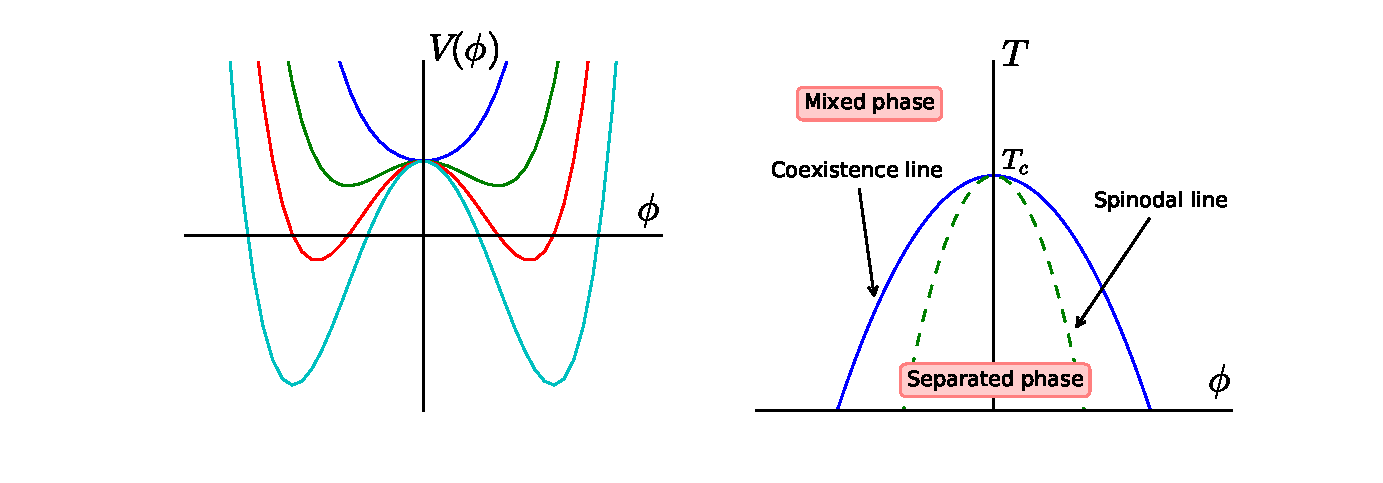
\includegraphics[width=0.9\textwidth]{figures/symmetric.eps}

\caption{Two panels showing (left) the form of the free energy density
$V(\phi)$ for the binary fluid for a number of different
temperatures. At temperatures above
the critical temperature, there is a single minimum (top curve), while
below $T_c$, two symmetric minima are present (lower curves). The related
phase diagram (right) in the temperature-composition plane shows mixed
and separated phases the boundary of which is the coexistence 
line. This (sometimes referred to as the binodal line) is the locus of
points which are the minima of $V(\phi)$ at different temperatures. The
spinodal line is formed by the locus of points which are the inflections
of $V(\phi)$.}
\label{figure-symmetric-schematic}
\end{figure}


If we consider a one-dimensional case, this is
\begin{equation}
A\phi + B\phi^3 - \kappa \frac{d^2 \phi}{dx^2} = 0.
\end{equation}
Note that the conservation of order parameter means this should be a
constrained minimisation, which can be handled by adding the
a Lagrange multiplier $\Lambda = \partial f / \partial \phi |_{\phi_0}$.
The resulting ordinary differential equation has a solution
$\phi(x) = \phi^\star \tanh(x/\xi)$ where $\xi$ is identified
as the interfacial width. It can be confirmed that this is a solution
if
\begin{equation}
\xi = (-2\kappa / A)^{1/2}.
\end{equation}
The one-dimensional case can also be used to determine the interfacial
tension, which is the excess energy associated with the interface.
If we denote the interfacial tension $\sigma$, then the excess
energy is
\begin{equation}
\sigma = \int_{-\infty}^{+\infty} \mathrm{d} x
\Big[
{\textstyle \frac{1}{2}} \kappa (d_x \phi)^2 + V(\phi) - V(\phi^\star)
\Big],
\end{equation}
which can be evaluated from the equilibrium profile with the interface
placed at the origin $\phi(x) = \phi^\star\tanh(x/\xi)$, along with a number
of standard integrals, to give
\begin{equation}
\sigma =  4\kappa\phi^{\star 2}/3\xi
 = \big(-8\kappa A^3/9B^2\big)^{1/2}.
\end{equation}
Further discussion of the practical choice of the free energy parameters,
and their
impact on interfacial width and tension is deferred until LATER.

\subsubsection{Dynamics}

In a purely diffusive regime, the time evolution of a conserved
order parameter may be expressed as the local divergence of a flux
$j_\alpha(\mathbf{r})$, that is,
$\partial_t \phi(\mathbf{r}) + \partial_\alpha j_\alpha(\mathbf{r}) = 0$.
In this picture, the system responds to small local changes in composition
by diffusion, which acts to reduce the energy. Formally, this
response of the free energy to a small change in composition is described
by the chemical potential
\begin{equation}
\mu = \frac{\delta F}{\delta \phi} = \frac{dV}{d\phi} - \kappa \partial_\alpha^2 \phi,
\end{equation}
being the functional derivative of the free energy with respect to the
order parameter. The dynamics is usually described in the context of the
model of Cahn and Hilliard \cite{cahn-hilliard-1958}, otherwise known as
Model B, where
\begin{equation}
\frac{\partial \phi}{\partial t} =
M\partial_\alpha^2 \frac{\delta F}{\delta \phi}.
\label{eq-cahn-hilliard}
\end{equation}
Here, the diffusive flux is related to the gradient of chemical potential
via $j_\alpha = -M \partial_\alpha \mu$, where $M$ is a mobilty
(taken to be uniform). 

In the presence of a fluid with velocity field $u_\alpha(\mathbf{r})$,
the full equation for the time evolution of the order parameter is
\begin{equation}
\partial_t \phi + \partial_\alpha (\phi u_\alpha + M\partial_\alpha \mu) = 0.
\label{eq-cahn-hilliard-final}
\end{equation}
This form again stresses the nature of the dynamics as a conservation law,
involving the divergence of advective fluxes $\phi u_\alpha$ and diffusive
fluxes $j_\alpha = -M\partial_\alpha \mu$. It
also admits that the mobility may be a function of position, e.g., via
$M = M(\phi)$. Equation~\ref{eq-cahn-hilliard-final} will form the basis of
the numerical solution of the binary fluid problem, coupled to the
Navier-Stokes equation.

The presence of a interface, or non-uniform composition, can lead to
thermodynamic stresses on the fluid which we denote $P_{\alpha\beta}$,
in additional to the usual viscous
stresses. The divergence of this
additional stress represents a body force density in the Navier-Stokes
equation, which is related to the chemical potential via
$f_\alpha = -\phi\partial_\alpha \mu = -\partial_\beta P_{\alpha\beta}$.
The full form of the additional stress may be related to the order
parameter by
\begin{equation}
P_{\alpha\beta} = p_0 \delta_{\alpha\beta}
  + \kappa \partial_\alpha \phi \partial_\beta \phi
\end{equation}
with isotropic contribution
\begin{equation}
p_0 = \phi \frac{dV(\phi)}{d\phi} -  V(\phi)
-\kappa\phi\partial_\alpha^2 \phi - \textstyle{\frac{1}{2}} \kappa (\partial_\alpha \phi)^2.
\end{equation}
Note that the stress $P_{\alpha\beta}$ is symmetric. At (local) equilibrium,
one expects gradients in the chemical potential to vanish,
and there will be neither diffusive fluxes ($j_\alpha = 0$) nor force on
the fluid ($f_\alpha = 0$).

\subsubsection{Surface (or wetting) free energy}

In the presence of a solid surface, the two component fluid gives
rise to the possiblity of a solid-fluid-fluid contact line. In the
symmetric case, the fluid-fluid interface will be at right angles to
a uniform flat surface. If one component wets the solid preferentially
(that is, it is energetically favourable for that component to be
in contact with the solid) the angle may move away from
90~degrees.
In general, the equilibrium contact angle $\theta$ is given by the
Young equation
\begin{equation}
\sigma_1 - \sigma_2 - \sigma \cos\theta = 0,
\end{equation}
where there are two solid-fluid surface tensions for components 1 and 2,
and the fluid-fluid interfacial tension is $\sigma$ as before.

This may be described in the free energy picture by adding a free
energy density per unit area assoicated with the surface:
\begin{equation}
f_s (\phi_s)= \textstyle{\frac{1}{2}} C \phi_s^2 + H \phi_s,
\end{equation}
where $\phi_s$ is the order parameter at the surface, and $C$ and $H$ are
constant parameters.

\subsection{Implementation}

\subsubsection{Lattice kinetic approach}

A second distribution function is introduced, denoted $g_i(\mathbf{r};t)$,
which describes the composition. The moments of this distribution, by
analogy with the hydrodynamic case with distribution
$f_i(\mathbf{r};t)$ given in
Eq.~\ref{equation-lb-f-moments}, are written
\begin{equation}
\phi(\mathbf{r};t) = \sum_i g_i (\mathbf{r};t), \quad
j_\alpha(\mathbf{r};t) = \sum_i g_i(\mathbf{r};t) c_{i\alpha}, \quad
\Phi_{\alpha\beta}(\mathbf{r};t) = \sum_i g_i(\mathbf{r};t)
c_{i\alpha}c_{i\beta}.
\end{equation}
Again, the summation is over index $i$ which counts the number of
discrete velocity components for the relevant lattice Boltzmann
model $N_{\mathrm{vel}}$. However, for the Cahn-Hilliard equation,
the only relevant physical moments are the order parameter
$\phi(\mathbf{r};t)$ and the flux $j_\alpha(\mathbf{r};t)$, so
the quantity $\Phi_{\alpha\beta}(\mathbf{r};t)$ is counted among
the kinetic modes and has no precise physical interpretation. In
contrast to the previous section, here $j_\alpha(\mathbf{r};t)$
is used to represent the total flux (advective
plus diffusive) rather than the purely diffusive flux.

The lack of direct physical interpretation for the second moment
means there are a number of possible choices at the collision
stage for the $g_i(\mathbf{r};t)$ distribution.
\begin{enumerate}
\item
Following Stratford \textit{et al.} \cite{j-stat-phys-2005}:
relax $j_\alpha$ toward the equilibrium $\phi u_\alpha$
at a rate related to the mobility and fix $\Phi_{\alpha\beta} =
\phi u_\alpha u_\beta + \mu \delta_{\alpha\beta}$.
\item
Following Kendon \textit{et al.} \cite{kendon2001}: fix both
$j_\alpha = \phi$ and
$\Phi_{} = \phi u_\alpha u_\beta + M\mu \delta_{\alpha\beta}$ so the
mobilty enters explicitly with the chemical potential.
\end{enumerate}

In both cases a reprojection is used to recover the post-collision
distributions $g_i^\star(\mathbf{r};t)$. This explicitly eliminates
kinetic modes other than $\Phi_{\alpha\beta}$. Hence
\begin{equation}
g_i = w_i \big(\phi + \phi u_\alpha c_{i\alpha}/c_s^2 +
(\mu\delta_{\alpha\beta} + \phi u_\alpha u_\beta) Q_{i\alpha\beta}/2c_s^4\big).
\end{equation}
In practice, this is not stable, and we use
\begin{equation}
g_i = \phi\delta_{i0} + w_i \big( j_\alpha c_{i\alpha} / c_s^2
+ \Phi_{\alpha\beta}Q_{i\alpha\beta} / 2c_s^4\big)
\end{equation}
where the $\delta_{i0}$ has the effect of moving most of the order
parameter into the non-propagating rest distribution $g_0$. 
This reprojection approach has the advantage that it eliminates several
spurious anisotropic terms which are introduced by a single relaxation
time approach (used by Kendon \textit{et al.}).

In the relaxation approach, the form of the relaxation for the
three components of the order parameter flux is
\begin{equation}
j_\alpha^\star =
j_\alpha - \tau_\phi^{-1} (j_\alpha - \phi u_\alpha),
\end{equation}
where $j_\alpha^\star$ is the post-collision flux and the relaxation
time $\tau_\phi$ is related to the mobility  via
\begin{equation}
\tau = {\textstyle\frac{1}{2}} + M\rho_0/\Delta t.
\end{equation}

\subsubsection{Finite difference approach}

For a number of reasons, it is advantageous to replace the lattice
kinetic approach by a conventional finite difference/finite volume
treatment of the Cahn-Hilliard equation
\begin{equation}
\partial_t \phi + \partial_\alpha ( \phi u_\alpha - M \partial_\alpha \mu) = 0.
\end{equation}
(Note that the finite difference and finite volume terminology will
be used somewhat interchanably here.) Briefly, the advantages are:
\begin{enumerate}
\item
The ambiguity in interpretation of the kinetic modes is avoided,
along with the corresponding computational overhead in memory and
memory movement.
\item
Additional features may be added to the Cahn-Hilliard equation more
easily. These might include a heterogeneous mobility $M=M(\phi)$, and
order parameter fluctuations (see below).
\end{enumerate}

\vfill
\pagebreak


\clearpage
\vfill\pagebreak
%%%%%%%%%%%%%%%%%%%%%%%%%%%%%%%%%%%%%%%%%%%%%%%%%%%%%%%%%%%%%%%%%%%%%%%%%%%%%%%
%
%  colloid.tex
%
%%%%%%%%%%%%%%%%%%%%%%%%%%%%%%%%%%%%%%%%%%%%%%%%%%%%%%%%%%%%%%%%%%%%%%%%%%%%%%%

\section{Colloid Examples}


\subsection{Initialisation from file}

We present a number of examples taken from the regression tests, the inputs
for which are found in
\begin{verbatim}
trunk/tests/regression
\end{verbatim}
For each test there is an input file, and an ASCII file containing the
details of the initial colloid state which is read at run time by means
of the key value pair
\begin{verbatim}
colloid_init    from_file
\end{verbatim}

A file of colloid information may be created with the utility
\begin{verbatim}
util/colloid_file.c
\end{verbatim}
As a minimum, this file must specify:
\begin{enumerate}
\item
A unique integer id for each particle;
\item
a radius and hydrodynamic radius $a_0$ and $a_h$ (use the same value
if unsure);
\item
an initial position ($x_{min} < x < x_{max}$) with $x_{min} = 0.5$
and $x_{max} = L_x + 0.5$ etc, where $L_x$ is the appropriate system
size for the problem at hand;
\item
the initial velocity etc may be safely initialised to zero.
\end{enumerate}
Note that is an inter-particle potential is to be specified at run time,
the initial position of the particles should not be so close that a
large force is experienced at time $t=0$. This can destabilise the
dynamics.

A single file of colloid information is produced in either ASCII or binary
format, which can be read in by specifying the appropriate
\begin{verbatim}
colloid_io_format_input   ASCII_SERIAL
\end{verbatim}
or \texttt{BINARY\_SERIAL} key value in both serial and parallel.


\subsubsection{Very short range potential}

See
\begin{verbatim}
tests/regression/test_spin_solid2_input
tests/regression/config.cds.init.001-001
tests/regression/test_spin_solid2_d3q19.ref*
\end{verbatim}

An example of a moderate volume fraction of particles is given for
a binary fluid undergoing spinodal decomposition. Here,
the capillary interaction between the neutrally wetting colloids
causes a strong effective attraction between particles. It is therefore
necessary to ensure the particles do not collide to the point of
overlapping at their hard-sphere radius. A counterbalancing short-range
soft-sphere potential is then defined in the input file:
\begin{verbatim}
soft_sphere_on 1
soft_sphere_epsilon 0.0004
soft_sphere_sigma 0.1
soft_sphere_nu 1.0
soft_sphere_cutoff 0.25
\end{verbatim}
where, following Eq.~\ref{eq_ss_shift}, we have
$v(r) \sim \epsilon (\sigma /r)^\nu$ ``cut-and-shifted'' so that
both potential and force smoothly match to zero at the cut-off
distance $r_c$ (here $0.25\Delta x$). The energy scale $\epsilon$
will need to be adjusted depending on the exact problem at hand
(here it will be related to the fluid-fluid interfacial tension).

Other relevant parameters here are
\begin{verbatim}
colloid_cell_min 8.0
lubrication_on 0
\end{verbatim}
which control, respectively, the minimum cell list width used to
help identify interactions, and the lubrication correction (here
switched off).


\subsubsection{Short-range potential}

See
\begin{verbatim}
tests/regression/test_yukawa_input
tests/regression/test_yukawa_cds.001-001
tests/regression/test_yukawa_d3q10.ref1
\end{verbatim}

This example involves a number of interacting particles in a simple
fluid including Brownian motion. The potential is Yukawa-like,
representative of a screened Coulomb interaction.

We have the parameters:
\begin{verbatim}
yukawa_on 1
yukawa_epsilon  1.330764285
yukawa_kappa 0.72463768115
yukawa_cutoff 16.0
\end{verbatim}
where the potential is $v(r) \sim \epsilon (-\kappa r) / r$. Again,
both potential and force are smoothly matched to zero at the
cut-off distance $r_c$ (here $r_c = 16\Delta x$). The relatively
long cut-off distance means that the minimum cell list cell width
must be correspondingly large (16 lattice units) which limits the
minimum parallel domain size.

This example also includes Brownian motion by means of fluctuating
hydrodynamics. The relevant parameters in the input are:
\begin{verbatim}
isothermal_fluctuations on 
temperature 0.0002133333
\end{verbatim}
Note that the \texttt{temperature} parameter here specifies
$k_BT = \langle c_x^2\rangle = \langle c_y^2 \rangle = \langle c_z^2 \rangle$
in three dimensions (at equilibrium);
this is reported in the output of the code at run time.

\subsubsection{Long range forces}

An Ewald sum is available for magnetic dipoles.


\clearpage
\vfill\pagebreak
%%%%%%%%%%%%%%%%%%%%%%%%%%%%%%%%%%%%%%%%%%%%%%%%%%%%%%%%%%%%%%%%%%%%%%%%%%%%%%%
%
%  liquidcrystal.tex
%
%  For nematics, cholesterics, blue phases based on the Landau
%  de Gennes approach.
%
%  Edinburgh Soft Matter and Statistical Physics Group and
%  Edinburgh Parallel Computing Centre
%
%  Contributing authors:
%  Kevin Stratford (kevin@epcc.ed.ac.uk)
%  Davide Marenduzzo was the source of the original LC approach.
%
%%%%%%%%%%%%%%%%%%%%%%%%%%%%%%%%%%%%%%%%%%%%%%%%%%%%%%%%%%%%%%%%%%%%%%%%%%%%%%%

\section{Liquid Crystals}
\label{section-lc}

\subsection{The Landau-de Gennes Approach}

\subsubsection{Tensor order parameter}

The liquid crystal order is described by a symmetric traceless tensor
$Q_{\alpha\beta}(\mathbf{r}; t)$. The largest eigenvalue and
associated eigenvector of $Q_{\alpha\beta}$ represent the magnitude
and local direction of liquid crystal molecular order. A theory based
on the tensor $Q_{\alpha\beta}$ has the advantage of being able to
describe disclinations where the local order vanishes and a director
is not defined. Readers are referred to, e.g., de Gennes and Prost
\cite{degennes-prost2002}, and Wright and Mermin \cite{wright-mermin}
for further information.

\subsubsection{Free Energy Density}

The free energy is a functional whose density
$f(Q_{\alpha\beta}, \partial_\gamma Q_{\alpha\beta})$
has bulk contributions depending on $Q_{\alpha\beta}$,
and elastic (distortion) contributions dependent on the
gradients of the order parameter
$\partial_\gamma Q_{\alpha\beta}$.

The bulk contributions are
\begin{equation}
\label{eq-lc-fed-bulk}
f(Q_{\alpha\beta}) =
{\textstyle\frac{1}{2}} A_0 (1 - \gamma / 3) Q_{\alpha\beta}^2
-{\textstyle\frac{1}{3}} A_0 \gamma Q_{\alpha\beta} Q_{\beta\pi} Q_{\pi\alpha}
+ {\textstyle\frac{1}{4}} A_0 \gamma (Q_{\alpha\beta}^2)^2.
\end{equation}
Here, $A_0$ is a constant which sets the overall energy scale; $\gamma$
is a temperature-like parameter which controls the position in the
phase diagram relative to the isotropic-nematic transition.

The bend, splay and twist distortions making up the gradient free
energy are modelled with two elastic
constants $\kappa_0$ and $\kappa_1$ as
\begin{equation}
f(\partial_\gamma Q_{\alpha\beta}) = 
{\textstyle\frac{1}{2}} \kappa_0 (\partial_\alpha Q_{\alpha\beta})^2
+ {\textstyle\frac{1}{2}} \kappa_1
(\epsilon_{\alpha\mu\nu} \partial_\mu Q_{\nu\beta} + 2q_0 Q_{\alpha\beta})^2.
\label{equation-lc-gradient-fe}
\end{equation}
Here, $\epsilon_{\alpha\mu\nu}$ is the permutation tensor and
$q_0 = 2\pi/p$ is a wavevector related to the pitch~$p$ of the
cholesteric. Setting $q_0 = 0$ permits a nematic state.
The one-constant approximation makes the simplification that
$\kappa_0 = \kappa_1 = \kappa$; the distinction between
$\kappa_0$ and $\kappa_1$ will be kept
in what follows unless otherwise stated.


\subsubsection{Molecular Field}

The molecular field $H_{\alpha\beta}$ is defined as the functional
derivative of the
free energy density with respect to the order parameter which here
gives
\begin{equation}
H_{\alpha\beta} = -\Bigg[
  \frac{\partial f(Q_{\alpha\beta})}{\partial Q_{\alpha\beta}}
- \partial_\gamma \frac{\partial f(\partial_\gamma Q_{\alpha\beta})}
{\partial Q_{\alpha\beta,\gamma}} \Bigg].
\end{equation}
In the absence of flow, the molecular field determines how the
order parameter relaxes toward equilibrium.

As the final expression for $H_{\alpha\beta}$ is somewhat complex, it
is useful to 
account for the individual terms here. First, the terms from the bulk free
energy density give rise to:
\begin{equation}
-A_0 (1 - \gamma/3) Q_{\alpha\beta} + A_0 \gamma Q_{\alpha\pi} Q_{\pi\beta}
- A_0 \gamma Q_{\pi\sigma}^2 Q_{\alpha\beta}.
\nonumber
\end{equation}
The second term in this expression
(arising from the cubic term in the free energy) is
forced to be traceless by subtracting one third of
Tr$(Q_{\alpha\pi}Q_{\pi\beta}) = Q_{\alpha\beta}^2$
so that we have
\begin{equation}
- A_0 (1 - \gamma/3) Q_{\alpha\beta}
+ A_0 \gamma (Q_{\alpha\pi} Q_{\pi\beta}
               - {\textstyle\frac{1}{3}} Q_{\pi\sigma}^2\delta_{\alpha\beta})
- A_0 \gamma Q_{\pi\sigma}^2 Q_{\alpha\beta}.
\nonumber
\end{equation}

The gradient term in $\kappa_0$, along with the first term in $\kappa_1$
arising from the expansion of the brackets in
Equation~\ref{equation-lc-gradient-fe}, give
\begin{equation}
\kappa_0 \partial_\alpha \partial_\gamma Q_{\gamma\beta}.
+
\kappa_1 \partial_\gamma
( \partial_\gamma Q_{\alpha\beta} - \partial_\alpha Q_{\gamma\beta}).
\nonumber
\end{equation}
Note that in the one constant approximation, this term collapses
to $\kappa \partial^2 Q_{\alpha\beta}$. The cross term in the expansion
of the brackets in~\ref{equation-lc-gradient-fe}, having been symmetrised,
contributes
\begin{equation}
-2\kappa_1 q_0
( \epsilon_{\alpha\mu\nu} \partial_\mu Q_{\nu\beta}
+ \epsilon_{\beta\mu\nu} \partial_\mu Q_{\nu\alpha}),
\nonumber
\end{equation}
which must again be forced to be traceless to give
\begin{equation}
-2\kappa_1 q_0 \big\{
( \epsilon_{\alpha\mu\nu} \partial_\mu Q_{\nu\beta}
+ \epsilon_{\beta\mu\nu} \partial_\mu Q_{\nu\alpha})
- {\textstyle\frac{1}{3}}( 
   \epsilon_{\pi\mu\nu} \partial_\mu Q_{\nu\pi}
  +\epsilon_{\pi\mu\nu} \partial_\mu Q_{\nu\pi} )
   \delta_{\alpha\beta} \big\}.
\nonumber
\end{equation}
The final term in is
$-4 \kappa_1 q_0^2 Q_{\alpha\beta}$. The complete expression for the molecular
field is then
\begin{eqnarray}
\label{eq-lc-h-full}
H_{\alpha\beta} &=&
- A_0 (1 - \gamma/3) Q_{\alpha\beta}
+ A_0 \gamma (Q_{\alpha\pi} Q_{\pi\beta}
               - {\textstyle\frac{1}{3}} Q_{\pi\sigma}^2\delta_{\alpha\beta})
- A_0 \gamma Q_{\pi\sigma}^2 Q_{\alpha\beta}
\nonumber\\
&&
+\kappa_0 \partial_\alpha \partial_\gamma Q_{\gamma\beta}
+
\kappa_1 \partial_\gamma
( \partial_\gamma Q_{\alpha\beta} - \partial_\alpha Q_{\gamma\beta})
\nonumber\\
&&
-2\kappa_1 q_0 \big(
( \epsilon_{\alpha\mu\nu} \partial_\mu Q_{\nu\beta}
+ \epsilon_{\beta\mu\nu} \partial_\mu Q_{\nu\alpha})
- {\textstyle\frac{1}{3}}( 
   \epsilon_{\pi\mu\nu} \partial_\mu Q_{\nu\pi}
  +\epsilon_{\pi\mu\nu} \partial_\mu Q_{\nu\pi} )
   \delta_{\alpha\beta} \big)
\nonumber\\
&& - 4 \kappa_1 q_0^2 Q_{\alpha\beta}.
\end{eqnarray}


\subsection{Surface Anchoring}

\label{section-lc-anchoring}

The preferred orientation of the liquid crystal fluid at a solid surface,
usually referred to as the surface anchoring, is relevant for both
solid walls and colloids.

\subsubsection{General boundary condition}

To impose a suitable boundary condition for the order parameter tensor
at a solid-fluid interface, we consider again the gradient terms in
the free energy
\begin{equation}
f (\partial_\gamma Q_{\alpha\beta}) = 
{\textstyle\frac{1}{2}} \kappa_0 (\partial_\beta Q_{\alpha\beta})^2
+ {\textstyle\frac{1}{2}}
 \kappa_1 (\epsilon_{\alpha\gamma\sigma} \partial_\gamma
Q_{\sigma\beta} + 2q_0 Q_{\alpha\beta})^2
\end{equation}
where we retain
two elastic constants $\kappa_0$ and $\kappa_1$;
the cholesteric pitch $p = 2\pi/q_0$.

Also relevant is a surface free energy (an area density), the exact form
of which is determined by the type of anchoring required. In general, we
expect this to depend on the order parameter, but not its gradients, so
write
\begin{equation}
f_s = f_s (Q_{\alpha\beta}, Q^0_{\alpha\beta})
\end{equation}
where $Q^0_{\alpha\beta}$ is some preferred order parameter configuration
at the surface (to be either normal or planar as discussed in the following
sections).

The boundary condition we wish to apply is derived from the Euler-Lagrange
equations, and for the fluid and surface terms gives rise to the equation
\begin{equation}
n_\gamma \frac{\partial f}{\partial Q_{\alpha\beta,\gamma}}
+ \frac{\partial f_s}{\partial Q_{\alpha\beta}} = 0,
\label{equation-lc-general-bc}
\end{equation}
where $n_\gamma$ is the outward unit normal at the surface (pointing into
the fluid). Note that the first term in the derivative of the fluid free
energy term with respect to
$Q_{\alpha\beta,\gamma}$ can be expended as
\begin{equation}
\kappa_0 n_\beta \partial_\gamma Q_{\alpha\gamma}
+ \kappa_1 n_\gamma
(\partial_\gamma Q_{\alpha\beta} - \partial_\alpha Q_{\gamma\beta})
- 2\kappa_1 q_0 n_\gamma \epsilon_{\alpha\gamma\sigma} Q_{\sigma\beta}.
\nonumber
\end{equation}
However, we should use a symmetric form (the derivative with respect to
$Q_{\beta\alpha,\gamma}$ is just as good) so we write this as:
\begin{eqnarray}
&
{\textstyle\frac{1}{2}} \kappa_0 (n_\alpha \partial_\gamma Q_{\beta\gamma}
+ n_\beta \partial_\gamma Q_{\alpha\gamma})
+ \kappa_1 n_\gamma \partial_\gamma Q_{\alpha\beta}
- {\textstyle\frac{1}{2}} \kappa_1 n_\gamma ( \partial_\alpha Q_{\gamma\beta}
+ \partial_\beta Q_{\gamma\alpha})
\nonumber
\\
&
- \kappa_1 q_0 n_\gamma (\epsilon_{\alpha\gamma\sigma} Q_{\sigma\beta}
+ \epsilon_{\beta\gamma\sigma}Q_{\sigma\alpha}).
\nonumber
\end{eqnarray}
The exact boundary condition will contain this term plus one
depending on the exact choice of the surface free energy which
describes a given anchoring condition.

\subsubsection{Normal or homeotropic anchoring}
The preferred direction of the surface order here is, as the name
suggests, normal to surface. We can write
\begin{equation}
f_s = {\textstyle\frac{1}{2}} w (Q_{\alpha\beta} - Q_{\alpha\beta}^0)^2
\end{equation}
where $w$ is a constant.
The preferred orientation $Q^0_{\alpha\beta}$ is based on the unit normal
at the surface $n_\gamma$, and is computed via the uniaxial approximation:
\begin{equation}
Q^0_{\alpha\beta}
= {\textstyle \frac{1}{2}} A (3n_\alpha n_\beta - \delta_{\alpha\beta}).
\end{equation}
The amplitude $A$ is provided by 
\begin{equation}
\label{equation-lc-amplitude}
A=\frac{2}{3}\left(\frac{1}{4}+\frac{3}{4}\sqrt{1 - \frac{8}{3\gamma}}\right).
\end{equation}
The full boundary condition for the gradient of the tensor order parameter
at the solid-fluid boundary from Equation~\ref{equation-lc-general-bc}
is then:
\begin{eqnarray}
{\textstyle\frac{1}{2}} \kappa_0 (n_\alpha \partial_\gamma Q_{\beta\gamma}
+ n_\beta \partial_\gamma Q_{\alpha\gamma})
+ \kappa_1 n_\gamma \partial_\gamma Q_{\alpha\beta}
- {\textstyle\frac{1}{2}} \kappa_1 n_\gamma ( \partial_\alpha Q_{\gamma\beta}
+ \partial_\beta Q_{\gamma\alpha})
\nonumber
\\
- \kappa_1 q_0 n_\gamma (\epsilon_{\alpha\gamma\sigma} Q_{\sigma\beta}
+ \epsilon_{\beta\gamma\sigma}Q_{\sigma\alpha})
- w(Q_{\alpha\beta} - Q_{\alpha\beta}^0) = 0.
\label{equation-lc-bc-normal}
\end{eqnarray}

\subsubsection{Planar (degenerate) anchoring}

For planar anchoring, the preferred orientation is in the local tangent
plane at the surface: this is a degenerate case as any orientation in
the plane is energetically equivalent. An appropriate boundary
condition is described by Fournier and Galatola \cite{fournier2005}
which we write as:
\begin{equation}
f_s =
{\textstyle\frac{1}{2}} w_1 (\tilde{Q}_{\alpha\beta} - \tilde{Q}^\perp_{\alpha\beta})^2
+ {\textstyle\frac{1}{2}} w_2 (\tilde{Q}_{\alpha\beta}^2 - A^2)^2.
\end{equation}
Here again, the amplitude $A$ is provided by
Equation~\ref{equation-lc-amplitude}. To compute this term we take
the local fluid order parameter $Q_{\alpha\beta}$, form the quantity
$$
\tilde{Q}_{\alpha\beta}
= Q_{\alpha\beta} + {\textstyle \frac{1}{2}A\delta_{\alpha\beta} }
$$
which is then projected onto the tangent plane via
$
\tilde{Q}^\perp_{\alpha\beta}
= P_{\alpha\gamma} \tilde{Q}_{\gamma\sigma} P_{\sigma\beta}
$
with the local surface normal entering through
$P_{\alpha\beta} = \delta_{\alpha\beta} - n_\alpha n_\beta$.
The full boundary condition resulting from
Equation~\ref{equation-lc-general-bc} is then
\begin{eqnarray}
{\textstyle\frac{1}{2}} \kappa_0 (n_\alpha \partial_\gamma Q_{\beta\gamma}
+ n_\beta \partial_\gamma Q_{\alpha\gamma})
+ \kappa_1 n_\gamma \partial_\gamma Q_{\alpha\beta}
- {\textstyle\frac{1}{2}} \kappa_1 n_\gamma ( \partial_\alpha Q_{\gamma\beta}
+ \partial_\beta Q_{\gamma\alpha})
\nonumber
\\
- \kappa_1 q_0 n_\gamma (\epsilon_{\alpha\gamma\sigma} Q_{\sigma\beta}
+ \epsilon_{\beta\gamma\sigma}Q_{\sigma\alpha})
- w_1 (\tilde{Q}_{\alpha\beta} - \tilde{Q}_{\alpha\beta}^\perp)
- 2w_2(\tilde{Q}_{\alpha\beta}^2 - A^2)\tilde{Q}_{\alpha\beta} = 0.
\label{equation-lc-bc-planar}
\end{eqnarray}



\subsection{Dynamics}

The time evolution of the orientational order parameter $Q_{\alpha\beta}$
in the presence of flow can be described by the Beris-Edwards equation
\cite{beris-edwards}.

\begin{equation}
\partial_t Q_{\alpha\beta} + \partial_\gamma (u_\gamma Q_{\alpha\beta})
+ S_{\alpha\beta}(W_{\alpha\beta}, Q_{\alpha\beta}) = -\Gamma  H_{\alpha\beta}.
\label{equation-lc-beris-edwards}
\end{equation}
This relates the time rate of change of the order parameter to terms
involving advection, the response to shear
$S_{\alpha\beta}(W_{\alpha\beta},Q_{\alpha\beta})$, and the molecular
field.

The advective term involves the fluid velocity $u_\alpha$ and the shear
term involves the velocity gradient tensor
$W_{\alpha\beta}= \partial_\beta u_\alpha$. The full definition of the
shear term is:
\begin{eqnarray}
S_{\alpha\beta} (W_{\alpha\beta}, Q_{\alpha\beta})
& = 
(\xi D_{\alpha\pi} + \Omega_{\alpha\pi})
(Q_{\pi\beta} + {\textstyle \frac{1}{3}} \delta_{\pi\beta})
+
(Q_{\alpha\pi} + {\textstyle \frac{1}{3}} \delta_{\alpha\pi})
(\xi D_{\pi\beta} - \Omega_{\pi\beta})
\nonumber\\
&-
2\xi(Q_{\alpha\beta} + {\textstyle\frac{1}{3}}\delta_{\alpha\beta})
Q_{\pi\sigma}W_{\sigma\pi}
\nonumber
\end{eqnarray}
where $D_{\alpha\beta} = \frac{1}{2}(W_{\alpha\beta} + W_{\beta\alpha})$ and
 $\Omega_{\alpha\beta} = \frac{1}{2}(W_{\alpha\beta} - W_{\beta\alpha})$
are the symmetric and antisymmetric contributions to the velocity gradient
tensor and $\xi$ is a material constant representing an effective
molecular aspect ratio.


The thermodynamic contribution to the stress on the fluid can be viewed as
the sum of three parts:
\begin{equation}
\Pi_{\alpha\beta} = \sigma_{\alpha\beta} + \tau_{\alpha\beta}
-
\partial_\alpha Q_{\pi\nu}
\frac{\delta {\cal F}}{ \delta \partial_\beta Q_{\pi\nu}}
\label{equation-lc-stress}
\end{equation}
where $\sigma_{\alpha\beta}$ and $\tau_{\alpha\beta}$ are the symmetric
and antisymmetric contributions from the liquid crystal order:
\begin{equation}
\sigma_{\alpha\beta} =
-p_0 \delta_{\alpha\beta} 
- \xi H_{\alpha\pi}(Q_{\pi\beta} + {\textstyle\frac{1}{3}}\delta_{\pi\beta})
- \xi (Q_{\alpha\pi} + {\textstyle\frac{1}{3}}\delta_{\alpha\pi}) H_{\pi\beta}
+ 2\xi (Q_{\alpha\beta} + {\textstyle \frac{1}{3}}\delta_{\alpha\beta} )
Q_{\pi\nu} H_{\pi\nu},
\end{equation}
where $p_0$ is the isotropic pressure, and
\begin{equation}
\tau_{\alpha\beta} = Q_{\alpha\pi} H_{\pi\beta} - H_{\alpha\pi} Q_{\pi\beta}. 
\end{equation}
The final term in Equation~\ref{equation-lc-stress} is expanded as
$$
-\kappa_0 \partial_\alpha Q_{\pi\beta} \partial_\nu Q_{\pi\nu}
-\kappa_1 \partial_\alpha Q_{\pi\nu}
\left[ \partial_\beta Q_{\pi\nu} - \partial_\pi Q_{\nu\beta}
+ 2q_0 \epsilon_{\gamma\beta\pi} Q_{\gamma\nu} \right].
$$


\subsubsection{Active stress}

An additional term may be added to the stress to model an active
apolar fluid. This term is
\begin{equation}
\Pi_{\alpha\beta}^a = -\zeta
(Q_{\alpha\beta} - {\textstyle\frac{1}{3}}\delta_{\alpha\beta})
\end{equation}
where $\zeta$ is an activity parameter: $\zeta < 0$ gives
contractile behaviour and $\zeta > 0$ gives extensile behaviour.

\subsection{Implementation}

\subsubsection{Fluid}

The time evolution of the order parameter is computed by a hybrid
approach where the hydrodynamics is in the LB sector, and the
Beris-Edwards Equation is solved in a finite difference approach.
The hydrodynamic quantities and the order parameter share the same
regular lattice. The velocity field, computed via LB, supplies
advective fluxes and the velocity gradient tensor using an appropriate
finite difference stencil.

Coupling to the Navier-Stokes equations is via a body force computed
locally at each lattice site via the divergence of the stress in
Equation~\ref{equation-lc-stress}.

It is also possible to compute solely relaxational dynamics where there
is no flow, and evolution only depends on the molecular field, and the
rotational diffusion constant.


\subsubsection{Solid}

First, we note that the assignment of solid and fluid lattice
nodes for the order parameter follows that for the density:
inside and outside are distinguished using the nominal radius
of the colloid $a_0$ and its position. It is useful, in addition,
to think about a series of control volumes surrounding each lattice
node whose faces are aligned with the lattice
(see Figure~\ref{figure-lc-hybrid}). A set of these
faces constitute the solid-fluid boundary in the hybrid picture.
Advective fluxes of order parameter are computed at the faces
of the control volumes, and the boundary condition is zero
normal flux at solid-fluid interfaces. Note that the colloid
is assumed to be stationary in assigning these fluxes.

\begin{figure}[h]
\begin{center}
%%%%%%%%%%%%%%%%%%%%%%%%%%%%%%%%%%%%%%%%%%%%%%%%%%%%%%%%%%%%%%%%%%%%%%%%%%%%%
%
%  hybrid.tex
%
%  Description of  LB-FD hybrid considerations.
%
%%%%%%%%%%%%%%%%%%%%%%%%%%%%%%%%%%%%%%%%%%%%%%%%%%%%%%%%%%%%%%%%%%%%%%%%%%%%%

\section{BBL and hybrid dynamics}

[I assume this will be preceded by some description of the
governing equations for the tensor order parameter and their
treatment.]

The well-established procedure of bounce-back on links (BBL)
\cite{Ladd04, nguyen} has been employed for the representation
of the colloids as moving solid objects within the LBM.
In the hybrid LB/FD approach used here, BBL is retained for
the distributions, which are simply reflected at the solid-fluid
surface with a correction which depends on the local surface
velocity (see Figure Xa). The resulting change in momentum is
summed over the links to give the net hydrodynamic
force on the colloid, which is then used to update the
particle velocity, and
hence position, in a molecular dynamics-like step. Boundary
conditions for the finite difference equations for the order
parameter tensor are dealt with in a different way.

First, we note that the assignment of solid and fluid lattice
nodes for the order parameter follows that for the density:
inside and outside are distinguished using the nominal radius
of the colloid $a_0$ and its position. It is useful, in addition,
to think about a series of control volumes surrounding each lattice
node whose faces are aligned with the lattice (Figure Xb). A set of
these
faces constitute the solid-fluid boundary in the hybrid picture.

Boundary conditions for $Q_{\alpha\beta}$ are of two types:
homeotropic, where the director  $n_\alpha^0$ is aligned with
the local unit normal to the surface $\hat{n}_\alpha$, and planar,
where the director lies in the plane of the tangent to the
surface. For either choice of director at the surface, we
may set the corresponding value of $Q_{\alpha\beta}$ at
lattice nodes immediately inside the surface via
\begin{equation}
Q_{\alpha\beta}^0 = S^0 (n_\alpha^0 n_\beta^0
- {\scriptstyle\frac{1}{3}}\delta_{\alpha\beta})
\end{equation}
where the constant $S^0$ controls the degree of surface order.
This allows us
to compute, at all fluid nodes, the derivatives
$\nabla_\gamma Q_{\alpha\beta}$ and $\nabla^2 Q_{\alpha\beta}$
using the same finite difference stencil. This allows the
molecular field and hence the diffusive terms in the Beris
Edwards equation to be computed.

Also appearing in the Beris-Edwards equations is the velocity
gradient tensor, which can be handled in a similar fashion
close to the colloid. The velocity field at solid nodes
immediately inside the colloid surface are set to the solid
body velocity $\bf{u} + \bf{\Omega} \times \bf{r}$. Again,
the velocity gradient tensor $\partial_\alpha u_\beta$ may
be computed using the same stencil at all fluid nodes.

Advective fluxes of order parameter are computed at the faces
of the control volumes, and the boundary condition is zero
normal flux at solid-fluid interfaces. Note that the colloid
is assumed to be stationary in assigning these fluxes.

The force on the fluid originating from the order parameter
is computed via the discrete divergence of the stress
$P_{\alpha\beta}$. In the fluid, this is implemented by
interpolating $P_{\alpha\beta}$ to the control volume faces
and taking differences between faces in each direction. This
method has the advantage that, with the introduction of colloids,
an interpolation/extrapolation of $P_{\alpha\beta}$ to the
solid-fluid boundary is possible. This allows one to compute the
divergence of the stress at fluid nodes adjacent to the colloid
in the normal way. At the same time, the discrete equivalent of
\begin{equation}
F_\alpha^\mathrm{coll} = \int P_{\alpha\beta} \hat{n}_\beta dS
\end{equation}
by summing $P_{\alpha\beta}$ over the relevant solid-fluid control
volume faces. By construction, this ensures that momentum lost by
the fluid is gained by the colloid, i.e., global momentum is
conserved.

Finally, movement of the colloid across the lattice is accompanied
by changes in its discrete shape. The events necessitate the
removal or replacement of fluid information. For the replacement
of fluid at newly exposed lattice nodes, this means an
interpolation of nearby order parameter values in the fluid to
provide the new information. This is analogous to what is done
for the LB distributions.


\begin{figure}[h]
\begin{center}

%\input{/home/kevin/doc/rgrid/xfig/hybrid1.epic}
\input{hybrid2.epic}
\end{center}
\caption{The colloid (represented by the solid circle) moves continuously
across the lattice. Lattice sites inside are designated solid, and those
outside fluid (open and closed points, respectively). In the lattice
Boltzmann picture (left) the surface is defined by a set of links
$f_b$, which involve discrete vectors $\mathbf{c}_b \Delta t$ which
connect fluid and solid sites. For the order parameter (right), the
colloid is represented by the set of faces, e.g., that between sites
$i,j$ and $i+1,j$ with unit normal $\hat{n_x}$. Discretisation effects
are found to be negigible for radii greater than about 5 lattice units.}
\end{figure}

\end{center}
\caption{The hybrid picture. In the lattice
Boltzmann picture (left) a surface is defined by a set of links
$f_b$, which involve discrete vectors $\mathbf{c}_b \Delta t$ which
connect fluid and solid sites. For the order parameter (right), the
colloid is represented by the set of faces, e.g., that between sites
$i,j$ and $i+1,j$ with unit normal $\hat{n}_x$. This is a rather small
colloid.}
\label{figure-lc-hybrid}
\end{figure}

The net hydrodynamic force on the colloid is computed via BBL
in the usual way. As discussed above, the force on the fluid
originating from the order parameter is computed via the
discrete divergence of the stress $\Pi_{\alpha\beta}$. In the
fluid, this is implemented by interpolating $\Pi_{\alpha\beta}$
to the control volume faces and taking differences between faces
in each direction. This method has the advantage that, with the
introduction of solid faces, an extrapolation of $\Pi_{\alpha\beta}$
to the solid-fluid boundary is possible. This allows one to compute
the divergence of the stress at fluid nodes adjacent to the colloid
in the normal way. At the same time, the discrete equivalent of
\begin{equation}
F_\alpha^\mathrm{coll} = \int \Pi_{\alpha\beta} \hat{n}_\beta dS
\end{equation}
may be found by summing $\Pi_{\alpha\beta}$ over the relevant solid-fluid
control volume faces. By construction, this ensures that momentum lost by
the fluid is gained by the colloid, i.e., global momentum is
conserved.

Finally, movement of the colloid across the lattice is accompanied
by changes in its discrete shape. When fluid sites are destroyed,
corresponding order parameter information is also lost. If new
fluid sites are created, new order parameter information may be
added locally either by interpolation from nearby fluid sites, or
from geometrical information from the local surface anchoring.


\subsubsection{Boundary conditions}

\begin{table}[t]
\centering
\tabcolsep=4pt
\begin{tabular}{|c|cccccc|}
\hline
&
$Q_{xx,x}$ & $Q_{xy,x}$ & $Q_{xz,x}$ & $Q_{yy,x}$ & $Q_{yz,x}$ & $Q_{zz,x}$\\
\hline
$Q_{xx}$ &
$\kappa_0 n_x$ & $-\kappa_1 n_y$ & $-\kappa_1 n_z$ & & &\\
$Q_{xy}$ &
$\kappa_0 n_y$ & $\kappa' n_x$ & & $-\kappa_1 n_y$  & $-\kappa_1 n_z$ & \\
$Q_{xz}$ &
$\kappa_0 n_z$ & & $\kappa' n_x$ & & $-\kappa_1 n_y$ &$ -\kappa_1 n_z$\\
$Q_{yy}$ &
 & $\kappa_0 n_y$ & & $\kappa_1 n_x$ & &\\
$Q_{yz}$ &
 & $\kappa_0 n_z$ & $\kappa_0 n_y$ & & $2\kappa_1 n_x$ & \\
$Q_{zz}$ &
 & & $\kappa_0 n_z$ & & & $\kappa_1 n_x$\\
\hline
\hline
&
$Q_{xx,y}$ & $Q_{xy,y}$ & $Q_{xz,y}$ & $Q_{yy,y}$ & $Q_{yz,y}$ & $Q_{zz,y}$\\
\hline
$Q_{xx}$ &
$\kappa_1 n_y$ & $\kappa_0 n_x$ & & & &\\
$Q_{xy}$ &
$-\kappa_1 n_x$ & $\kappa' n_y$ & $-\kappa_1 n_z$ & $\kappa_0 n_x$ & &\\
$Q_{xz}$ &
 & $\kappa_0 n_z$ & $2\kappa_1 n_y$ & & $\kappa_0 n_x$ & \\
$Q_{yy}$ &
 & $-\kappa_1 n_x$ & & $\kappa_0 n_y$ & $-\kappa_1 n_z$ & \\
$Q_{yz}$ &
 & & $-\kappa_1 n_x$ & $\kappa_0 n_z$ & $\kappa' n_y$ & $-\kappa_1 n_z$\\
$Q_{zz}$ &
 & & & & $\kappa_0 n_z$ & $\kappa_1 n_y$\\
\hline
\hline
&
$Q_{xx,z}$ & $Q_{xy,z}$ & $Q_{xz,z}$ & $Q_{yy,z}$ & $Q_{yz,z}$ & $Q_{zz,z}$\\
\hline
$Q_{xx}$ &
$\kappa_1 n_z$ & & $\kappa_0 n_x$ & & & \\
$Q_{xy}$ &
 & $2\kappa_1 n_z$ & $\kappa_0 n_y$ & & $\kappa_0 n_x$ & \\
$Q_{xz}$ &
$-\kappa_1 n_x$ & $-\kappa_1 n_y$ & $\kappa' n_z$ & & & $\kappa_0 n_x$  \\
$Q_{yy}$ &
 & & & $\kappa_1 n_z$ & $\kappa_0 n_y$ & \\
$Q_{yz}$ &
 & $-\kappa_1 n_x$ & & $-\kappa_1 n_y$ & $\kappa' n_z$ & $\kappa_0 n_y$ \\
$Q_{zz}$ &
 & & $-\kappa_1 n_x$ & & $-\kappa_1 n_y $ & $\kappa_0 n_z$\\
\hline
\end{tabular}
\caption{Coefficients of the various derivatives of the order parameter
tensor appearing in six equations for the elements of the
order parameter (including $Q_{zz}$).
Note $\kappa_0 + \kappa_1 = \kappa'$ and all the
coefficients have been multiplied by a factor of 2 in the off-diagonal
equations.}
\label{table-lc-bc}
\end{table} 


In three dimensions, the boundary condition Eq.~\ref{equation-lc-general-bc}
provides six equations containing (potentially) 18 unknown derivatives
$\partial_\gamma Q_{\alpha\beta}$
corresponding to the 6 elements of the order parameter
tensor $Q_{xx}$, $Q_{xy}$, $Q_{xz}$, $Q_{yy}$, $Q_{yz}$, $Q_{zz}$.
While the equation corresponding to $Q_{zz}$ must appear to
retain isotropy, $Q_{zz}$ itself, and its derivatives, may be
replaced via the
constraint on the trace of $Q_{\alpha\beta}$. We can therefore either
solve a fully determined system including $Q_{zz}$, and then impose
tracelessness on the result, or replace $Q_{zz}$ and solve six
equations for five unknowns, with the sixth equation acting as the
constraint. These methods provide the same answer for cases where
the surface normal is along the coordinate directions.

In general, Equation~\ref{equation-lc-general-bc} is slightly
cumbersome: the coefficients of the various derivatives for each
of the six equations are shown in Table~\ref{table-lc-bc}. As an
concrete example,
at a flat surface with normal anchoring and, e.g., $n = (1, 0, 0)$,
the number of unknowns (six) are the gradients $\partial_x Q_{\alpha\beta}$
at the boundary --- we assume the tangential gradients
$\partial_y Q_{\alpha\beta}$
and $\partial_z Q_{\alpha\beta}$ can be approximated
using the standard differencing method involving only fluid values of
$Q_{\alpha\beta}$. We proceed by
computing the constant terms relevant for normal anchoring
$$
- \kappa_1 q_0 n_\gamma (\epsilon_{\alpha\gamma\sigma} Q_{\sigma\beta}
+ \epsilon_{\beta\gamma\sigma}Q_{\sigma\alpha})
- w(Q_{\alpha\beta} - Q_{\alpha\beta}^0)
$$
using $Q_{\alpha\beta}$ from the adjacent fluid site. To these
constant terms are added the tangential gradients.
The gradients at the surface are then computed by solving a 6x6
linear algebra problem for $\partial_x Q_{\alpha\beta}$. This
allows the full gradient at the adjacent fluid site to be constructed.

At concave edges or corners, where it is not possible to compute the
tangential gradients from the usual stencil as for a flat interface,
a different approach is required. Here, either a 12$\times$12 or
18$\times$18 system of equations is solved containing the relevant
unknown coefficients from Table~\ref{table-lc-bc} and the relevant
constant terms computed as before.





\vfill
\pagebreak


\clearpage
\vfill\pagebreak
\section{Polar Active Gel}


Here we consider a polar vector field model to study active gels. 
The order parameter is this time a vector $P_\alpha$
(with variable magnitude) as there is no longer head-tail symmetry
in the system as was the case for the ${\bf Q}$ tensor formulation. 
The equation of motion as:
\begin{equation}
\partial_t P_\alpha  \partial_\beta (u_{\beta} + wP_{\beta}) P_{\alpha}
= \lambda D_{\alpha\beta} P_{\beta} - \omega_{\alpha\beta} P_{\beta}
+\Gamma' h_{\alpha}.
\end{equation}

In this equation, $w$ is an active term, due to swimming, which causes
self-advection of the order parameter, while $\lambda$ is a material
dependent constant -- positive for rod-like molecules. If $|\lambda|>1$
the liquid crystalline passive phase is flow-aligning, otherwise it is
flow-tumbling. 

Note that the convection for the Leslie-Ericksen is that the
velocity gradient tensor should be writen $W_{\alpha\beta}
= \partial_\alpha u_\beta$ (and not the other way round, which
is usual).

The molecular field is given by
$h_{\alpha}=-\delta {\cal F}_{\rm pol}/\delta p_{\alpha}$
where ${\cal F}_{\rm pol}$ is the free energy for a polar active nematic,
whose density we can take to be:
\begin{equation}
f =  \frac{\alpha_2}{2} |{\mathbf P}|^2 + \frac{\alpha_4}{4}|{\mathbf P}|^4
+ \frac{K}{2}\left(\partial_\alpha P_{\beta}\right)^2 + 
\frac{K_{LC}}{2}\left[\partial_\alpha (P_{\beta}P_{\gamma})\right]^2 
\end{equation}
where $K$ and $K_{LC}$ are elastic constants, $\alpha_4>0$, and $\alpha_2$ 
can be positive (isotropic phase) or negative (polar nematic phase).

The molecular field is explicitly given by:
\begin{equation}
h_{\alpha}=-\alpha_2 P_{\alpha} -\alpha_4 P_{\alpha} P_{\beta}P_{\beta}+
K \partial_{\beta}\partial_{\beta} P_{\alpha}+2 K_{LC}
P_{\gamma}\partial_{\beta}\partial_{\beta} (P_{\gamma}P_{\alpha}).
\end{equation}


The Navier-Stokes equation is:
\begin{equation}
\rho \left(\partial_t+v_{\beta}\partial_{\beta}\right) v_{\alpha} =
\partial_{\beta} \Pi_{\alpha\beta} 
+\eta \partial_{\beta}\partial_{\beta} v_{\alpha}.
\end{equation}


The stress tensor this time is 
\begin{eqnarray}
\Pi_{\alpha\beta} =
\frac{1}{2}\left(P_\alpha h_\beta - P_\beta h_\alpha \right)
- \lambda\left( (P_\alpha h_\beta + P_\beta h_\alpha)/2 
- (1/3)P_\gamma P_\gamma \delta_{\alpha\beta} \right)
\\
-  \zeta ( P_\alpha P_\beta - (1/3)P_\gamma P_\gamma \delta_{\alpha\beta})
- K \partial_\alpha P_\gamma \partial_\beta P_\gamma.
\end{eqnarray}
The active term in the stress tensor, proportional
to $\zeta$, has the same form for apolar and polar active gels. 

\subsection{User input}

\inputkey{free\_energy polar\_active}

This models a polar active gel with vector order parameter $P_\alpha$.
The free energy density is:


The corresponding input parameters are:

\inputkey{polar\_active\_a}

\inputkey{polar\_active\_b}

\inputkey{polar\_active\_k}

\inputkey{polar\_active\_klc}

\inputkey{polar\_active\_zeta}

\inputkey{polar\_active\_lambda}

\inputkey{leslie\_ericksen\_gamma}

\inputkey{leslie\_ericksen\_swim}




\clearpage
\vfill\pagebreak
%%%%%%%%%%%%%%%%%%%%%%%%%%%%%%%%%%%%%%%%%%%%%%%%%%%%%%%%%%%%%%%%%%%%%%%%%%%%%
%
%  porous.tex
%
%  Some considerations for porous media.
%
%  $Id$
%
%  Edinburgh Soft Matter and Statistical Physics Group and
%  Edinburgh Parallel Computing Centre
%
%  Kevin Stratford (kevin@epcc.ed.ac.uk)
%  (c) 2011 The University of Edinburgh
%
%%%%%%%%%%%%%%%%%%%%%%%%%%%%%%%%%%%%%%%%%%%%%%%%%%%%%%%%%%%%%%%%%%%%%%%%%%%%%



\section{Porous Media}

Porous media calculations can be undertaken when appropriate
solid/fluid status information is supplied. The are a number
of switches available in the input file:

\inputkey{porous\_media\_file}

specifies the file stub name to be read at the start of execution.
(If the stub name is \texttt{file} then the code will expect to
find \texttt{file.001-001} in the current directory.

\inputkey{porous\_media\_format}

is either \texttt{ASCII} or \texttt{BINARY} as appropriate. Note that
in parallel, a single data file can be supplied, but it must be binary.
The default is \texttt{BINARY}.

\inputkey{porous\_media\_type}

is either \texttt{status\_only} (the default) or \texttt{status\_with\_h}.

\subsection{File format}

In all cases the status (fluid/solid) information is represented by a
single \texttt{char} (or integer), which must be supplied via the
porous media file. A single file should contain data matching the
current system size, and have the $z-$direction running fastest,
followed by the $y-$direction. Note that in non-periodic directions,
the structure must be 'closed', i.e., all the points at the edge
should be solid.

Fluid sites are designated by \texttt{0} and boundary or solid sites
by \texttt{1}. These data should be of type \texttt{char} in binary,
and may be integer in ASCII.

Where wetting information is required, the free energy parameter $H$
can be supplied by using the \texttt{status\_with\_h} switch. In this
case, the \texttt{char} status is augmented by a single \texttt{double}
value which is the local value of $H$. The order is then
$s_1,h_1, s_2, h_2, \ldots$.

An example of how to construct a porous media file is provided in
\texttt{util/capillary.c}, which builds an appropriate file for
a square or circular capillary tube. Please see the comments in
the file for further details. Note that the allowed
solid/fluid status values are defined in \texttt{src/site\_map.h}.
A solid boundary is \texttt{BOUNDARY}, while fluid is \texttt{FLUID}.

\subsection{Permeability calculations}

Single fluid permeability calculations for a given proous structure
can be undertaken by driving a flow via the fluid body force. Note
that the structure must be periodic in the direction of the force
(this may mean duplicating a 'reflected' version of a given sample
to create the correct input). The body force can be specified so
that, e.g., to drive a flow in the positive $x-$direction

\texttt{force 0.001\_0.000\_0.000}

The force should not be so large that the maximum velocity generated
threatens the Mach number constraint. To get a measurement of the
flow at equilibrium, the calculation should be run at least the
momentum diffusion time for the system ($L^2/\eta$ in LB time steps).

The net flow can be measured by combining the statistics for the
total momemtum and the total density (which is equal to the volume
with $\rho_0 = 1$).

Note that in the case of porous media with narrow channels at the grid
scale, the wall velocity can be dependent on the viscosity of the fluid.
This is an artefact of the bounce-back on links and will result in a
viscosity-dependent permeability (see, e.g., \cite{lipanmiller}).
To minimise this effect, e.g.,  Ginzburg and d'Humi\`eres \cite{ginzburg}
corrects the viscosity-dependence of the apparent boundary position
using a three relaxation time scheme. This is currently under
investigation.


\subsection{Circular and rectangular capillaries}

\label{section:exact_conductance}

For an infinite  capillary of circular cross section radius $a$,
the conductance is known analytically\cite{papanastasiou}. The
flow per unit area $J$ is given by
\begin{equation}
J = - \frac{1}{8\eta} \frac{\partial p}{ \partial x} a^2. 
\end{equation}
If the pressure gradient is replaced by a uniform body force
$-\partial p/ \partial x = \rho g$, then one can define a
viscosity-independent conductance $C$ via $ J = C \rho g / \eta$,
i.e., $C = a^2/8$. So, by measuring the volume flux at steady state
for a fixed applied body force, one can compute an estimate of the
conductance to compare with this result.

An analtyical expression is also available for the conductance
of a square or rectugular capillary. For an infinite capillary
of square cross section width $w \times h$ (where $h$ is the
longer),
the volume flux per unit area $J$ is expected to be
\cite{papanastasiou,edo1}
\begin{equation}
J = - \frac{1}{3\eta} \frac{\partial p}{\partial x} (h/2)^2
\left[
1 - 6(h/w) \sum_{k=1}^{\infty} \frac{\tanh(\alpha_k w/h)}{\alpha_k^5} 
\right]
\end{equation}
where $\alpha_k = (2k - 1)\pi/2$. The pressure gradient
$-\partial p / \partial x$ is replaced by the body force $\rho g$ and
one can difine the viscosity-independnet conductance $C$ via
$J = C\rho g / \eta$. The calculation procedes as above.

\subsection{Worked example}

\subsubsection{Setting up the structure}

We will work out the conductance of a simple one-dimensional capillary
of circular cross section. We can set up the structure using the
utility program found in \texttt{util/capillary.c}.

We set the system size to be $(10,10,32)$ in the $x-$, $y-$, and
$z-$directions, respectively. The cross section in $x-y$ will be
a discrete  approximation to a circle. The nominal radius is
$a = 4$ lattice units (allowing for solid sites at each edge).
In \texttt{capillary.c} we
set
\begin{verbatim}
const int xmax = 10;
const int ymax = 10;
const int zmax = 32;
\end{verbatim}
Note that the conductance should be independent of the length of the
capillary in the $z-$direction. We will check this later.

We choose a circular cross section via:
\begin{verbatim}
enum {CIRCLE, SQUARE};
const int xsection = CIRCLE;
\end{verbatim}
For this problem, the wetting parameters are irrelevant, and can be
ignored. In addition we set
\begin{verbatim}
enum {STATUS_ONLY, STATUS_WITH_H};
const int output_type = STATUS_ONLY;
\end{verbatim}
to specify that the output will contain only the structural information.
The output filename containing the structure is set via
\begin{verbatim}
const char * filename = "capillary.001-001";
\end{verbatim}

The program may be compiled and run via
\begin{verbatim}
$ gcc capillary.c -lm
$ ./a.out
\end{verbatim}
The output provides a simple representation of the cross section,
and a count of the number of solid sites, the number of fluid sites,
and the total. Again, the wetting parameters are irrelevant. For this
case we have
\begin{verbatim}
Cross section (0 = fluid, 1 = solid)
 1 1 1 1 1 1 1 1 1 1
 1 1 1 0 0 0 0 1 1 1
 1 1 0 0 0 0 0 0 1 1
 1 0 0 0 0 0 0 0 0 1
 1 0 0 0 0 0 0 0 0 1
 1 0 0 0 0 0 0 0 0 1
 1 0 0 0 0 0 0 0 0 1
 1 1 0 0 0 0 0 0 1 1
 1 1 1 0 0 0 0 1 1 1
 1 1 1 1 1 1 1 1 1 1
n = 3200 nsolid = 1536 nfluid = 1664
\end{verbatim}
Note that the outermost sites in each direction here are solid. There
should be a file \texttt{capillary.001-001} in the current directory.
This should be moved to the executable directory.


\subsubsection{Setting up the input}

Assuming we have compiled the serial code, we must now set up the
input file to be consistent with the capillary structure we want
to use. The \texttt{src/input.ref} file can be used as a template.
We should set the system size
\begin{verbatim}
size 10_10_32
\end{verbatim}
The location of the porous media file is specified using
\begin{verbatim}
porous_media_format BINARY
porous_media_file   capillary
porous_media_type   status_only
\end{verbatim}
Note that the extension \texttt{.001-001} of the filename has been
removed in the input file (it gets added back automatically by the
main code at run time).

As this is a single fluid calculation with no free energy involved
we must set
\begin{verbatim}
free_energy none
\end{verbatim}
What are the fluid parameters? We will set the viscosity to
$1/6$ in lattice units (and the bulk viscosity to the default
value by commenting it out; the default value is the same as
the shear viscosity):
\begin{verbatim}
viscosity 0.16666666666666666
#bulk_viscosity 0.1
\end{verbatim}
We expect that the number of time steps to reach a steady state
will be of order $t \approx a^2/\eta$, which we estimate using
$a=4$ so $t \approx 100$ LB time steps. We will try
\begin{verbatim}
N_cycles 200
\end{verbatim}
Note that we will need output on the total momentum of the system
as a function of time, so we set
\begin{verbatim}
freq_statistics 50
\end{verbatim}

Finally, we need to set a force in the $z-$direction to drive the
flow. Again, the final conductance should be indpendent of this
force providing the force is small enough that both the Mach number
and the Reynolds number are small compared to unity in steady stead.
We will set
\begin{verbatim}
force 0.00_0.00_0.0000001
\end{verbatim}

\subsubsection{Extracting the conductance}

With these parameters specified, we can run the code. The output
should reflect the parameters in the input file, and the time step
loop should start if the parameters, and the \texttt{capillary.001-001}
file has been read successfully. The code reports various fluid
properties. The density is \texttt{[rho]}, and we see that the
total is the same as the number of fluid sites reported by the
\texttt{capillary.c} program:
\begin{verbatim}
Scalars - total mean variance min max
[rho]    1664.00  1.00000000000-2.2204460e-16  1.00000000000 1.00000000000
\end{verbatim}
Note that the total density (ie., mass) should remain exactly unchanged
for the duration of the run; if not, there is something wrong.

The total momentum of the fluid in each coordinate direction is
reported, and we should see, as a function of time
\begin{verbatim}
Momentum - x y z
...
[fluid   ]  1.5321078e-14  1.8207658e-14  1.8529405e-03
[fluid   ] -8.2378548e-14  2.8865799e-15  1.9422398e-03
[fluid   ]  1.1302070e-13  6.1950445e-14  1.9467213e-03
[fluid   ]  2.4091840e-14  1.1102230e-16  1.9469462e-03
\end{verbatim}
Note as we have applied an external force in the $z-$direction,
the $z-$momentum increases with time while the momenutm in the
other two directions is constant (to machine accuracy, which is
around $10^{-16}$). Further, the $z-$momentum
is still changing slightly after 200 time steps, so we have
not run long enough to reach a steady state. If we run for
400 steps, we should see that the $z-$momentum is unchanged
over the last 100 time steps.
\begin{verbatim}
Momentum - x y z
...
[fluid   ]  1.0424994e-13  1.6098234e-14  1.9469580e-03
[fluid   ]  3.2973624e-14  3.2862602e-14  1.9469580e-03
\end{verbatim}
Finally, note the maximum velocity in the flow direction
is small compared with unity, and so both Mach number and
Reynolds number are also small in this case.


The figure we are interested in is the total momentum in the
$z-$direction which is $1.947\times 10^{-3}$. As the mean
density is unity, this is also the average total volume flux $J_v$.
The volume flux per unit area $J = J_v / a^2 L_z$, where $a^2 L_z$
is the volume of the discrete system (1664 in lattice units).
Following section \ref{section:exact_conductance},
we can write a viscosity independent conductance
$C = J\eta / \rho g$, with $g$ the force in the $z-$direction.
Putting all this together, we have $C = (1.947\times 10^{-3} / 1664)
\times (1/6) / (1.0 \times 1\times 10^{-7}) = 1.950$. The theoretical
figure is $C = 2$, so the simulation is correct to within a discretisation
error of about 3\%. Better accuracy may be acheived by increasing the
resolution of the circle; e.g., for $a = 8$, the result is 8.043 versus
an exact result of $C = 8$ --- an error of around 0.5\%.

\subsubsection{In parallel}

We can run the same calculation using the parallel code (recompile
with \texttt{make mpi}). In the input file we set
\begin{verbatim}
size 10_10_32
grid 1_1_2
\end{verbatim}
to set the parallel decomposition explicitly to two MPI tasks in the
$z-$direction. We also set
\begin{verbatim}
porous_media_format BINARY_SERIAL
porous_media_file   capillary
porous_media_type   status_only
\end{verbatim}
to ensure the structure file is read correctly in parallel.
We should run this on 2 MPI tasks, e.g.,
\begin{verbatim}
$ mpirun -np 2 ./Ludwig.exe input
\end{verbatim}
The final result should be exactly the same as the serial version
to machine accuracy. You may also be able to spot that the execution
time is approximately half that for the serial version (although this
problem is a little small for efficient parallelisation).

\subsubsection{General porous media}

For a general porous media, we can make use of Darcy's Law which
defines a permeability $k$ (with dimensions of area) via
\begin{equation}
J_v = - \frac{k A}{\eta} \frac{\partial P}{\partial z}
\end{equation}
where $J_v$ is the volume flux, $A$ is the cross-sectional area
of the sample, and $\partial P / \partial z$ is the pressure gradient
as before. 


\subsubsection{Matching lattice and real units in porous media}


Following Succi \cite{succi} (Chapter~8) the following argument
can be made to match lattice quantities and real physical
quantities for a given system of interest.
Dimensionless lattice Boltzmann units set the lattice spacing
$\Delta x = 1$, the lattice time step $\Delta t = 1$ and the
mean density of the fluid to $\rho_0 = 1$. The speed of sound
in lattice units is $c_s = 1/ \sqrt{3}$. How do we match these
units to physical ones?

Suppose we have discretised an X-ray tomography image with a resolution
of 1 voxel equal to 1 $\mu$m. If we represent one voxel by one cubic
lattice with width $\Delta x$, then we can match $\Delta x = 1\mu$m. A
large data set might provide 1000 voxels on a side, giving
1000 lattice sites, which would represent 1 mm.
Similarly, if our real system is water at room temperature with density
$\rho = 1000$kg~m$^{-3}$, then we may equate the lattice density
$\rho_0 = 1$ to be equivalent to 1000~kg~m$^{-3}$. (This means the
mass of fluid at one lattice site of volume $\Delta x^3 = 1 \mu$m$^{3}$
is then 10$^{-15}$~kg, although this is not a very useful number.)

This leaves time. This is matched via the speed of sound. For the real
system, we take the speed of sound in water at 20$^o$C to be
1480 m~s$^{-1}$. So the speed of sound on the lattice
$(1/\sqrt{3}) \Delta x$ per $\Delta t$ matches 1480~m~s$^{-1}$,
or $\Delta t = 1/\sqrt{3} \times 10^{-6} / 1480 \approx 3.9 \times 10^{-10}$s.
Note that this is a small unit, i.e., it would require very many time
steps to reach a `macroscopic' time in any simulation.

We should also consider the Reynolds number $Re = \rho U L / \eta$.
Suppose our real structure has a characteristic pore size which is
just at the resolution of the X-ray tomography image: $L = h = 1\mu$m.
If the fluid (water) has viscosity $\eta = 10^{-3}$ Pa s, and
a typical flow is $U \sim 10^{-3}$ m~s$^{-1}$, then the pore scale
Reynolds number is $Re_h \sim 10^{-3}$. In the LB, if we choose a
lattice viscosity $\eta = 1/6$, and generate a typical flow in
lattice units of $10^{-4}$, then the Reynolds number in the
simulation (with $\rho_0 = 1$ and $L = \Delta x = 1$) is
$Re \sim 6 \times 10^{-4}$, which is similar.


There is one potential problem if we wish to study transport
phemonema where we might want to run a simulation long enough
for the flow to cross the whole sample. With $U \sim 10^{-4}$
in lattice units and a large sample size of, say,  1024$^3$ the
flow would take around 10$^7$ simulation time steps to propagate
information across the system. This is computationally expensive.
One solution is
to artificially raise the flow speed (and hence the Reynolds
number). This is acceptable as long as the Reynolds number
remains small compared with unity (all Reynolds numbers $< 0.1$
can be regarded as neglible \cite{batchelor}.) Here, for example,
if we raise the flow by two orders of magnitude to $10^{-2}$ in
lattice units,
the Reynolds number is still acceptable at $Re = 6\times 10^{-2}$,
and the number of simulation time steps is reduced to a more
managable $10^5$ (see also \cite{cates_scaling}).



\clearpage
\vfill\pagebreak
%%%%%%%%%%%%%%%%%%%%%%%%%%%%%%%%%%%%%%%%%%%%%%%%%%%%%%%%%%%%%%%%%%%%%%%%%%%%%%
%
%  surfactant.tex
%
%  Some notes on surfactant work
%
%%%%%%%%%%%%%%%%%%%%%%%%%%%%%%%%%%%%%%%%%%%%%%%%%%%%%%%%%%%%%%%%%%%%%%%%%%%%%%

\section{Surfactants}

This section describes the approach taken to study surfactants. Here,
we always adopt the hydrid method, i.e., LB for the hydrodynmic
equations and finite difference for the associated Cahn-Hilliard
equations. Coupling between the two sectors is via the velocity
field and the external force on the fluid computed via the
divergence of the `chemical stress'.

In this model the surfactant appears as a concentration field
$\psi(\mathbf{r};t)$, alongside the compositional order parameter
$\phi(\mathbf{r};t)$ as appears in the binary fluid. There are
two corresponding Cahn-Hilliard equations: first,

\begin{equation}
\partial_t \phi + \partial_\alpha \phi u_\alpha = 
\partial_\alpha M_\phi \partial_\alpha \mu_\phi,
\end{equation}
and second
\begin{equation}
\partial_t \psi + \partial_\alpha \psi u_\alpha = 
\partial_\alpha M_\psi \partial_\alpha \mu_\psi.
\end{equation}

\subsection{Free Energy}

A number of different free energies have been used to study
surfactants [cite Yeomans]. Here, the free energy is based on
that used by van der Graff and van der Sman and others [cite].
There are a number of different contributions to the free
energy density:
\begin{equation}
f = f_\phi + f_\psi +f_1 + f_{ex}.
\end{equation}
The first is exactly that used for the binary fluid, i.e.,
\begin{equation}
f_\phi (\phi, \partial_\alpha\phi) =
{\textstyle \frac{1}{2}} A \phi^2 + {\textstyle \frac{1}{4}} B \phi^4
+ {\textstyle \frac{1}{2}} \kappa (\partial_\alpha \phi)^2.
\end{equation}
The surface tension and the interfacial width are determined from the
choice of parameters $A,B,\kappa$ as before.
The second term in the free energy density
represents the entropic
energy of mixing of the surfactant with the bulk phases
\begin{equation}
f_\psi (\psi) = kT \left[ \psi \ln\psi + (1 - \psi)\ln(1-\psi) \right]
\end{equation}
where the parameter $kT$ sets the energy scale for the whole system.
The surfactant order parameter, $\psi$, is unity for a saturated
interface and zero for a plain interface.

The surfactant lowers the energy of the interface where it is adsorbed
there, represented by the term
\begin{equation}
f_1(\psi, \partial_\alpha \phi) 
= -{\textstyle \frac{1}{2}} \epsilon \psi (\partial_\alpha \phi)^2
  -{\textstyle \frac{1}{2}} \beta  \psi^2 (\partial_\alpha \phi)^2
\end{equation}
where $\epsilon$ and $\beta$ are parameters. Note that only the
first term appears in \cite{vandergraaf}, while the second term is
based on that appearing in, e.g., \cite{diamant}. If $\beta = 0$,
the surfactant profile at the interface is symmetric (so-called
Langmuir adsoption) whereas the term in $\beta$ induces an
asymmetry (Frumpkin adsorption).
Finally,  $f_{ex}$ is [van der Sman claims]
an enthalpic contribution introduced 
to stabilise the interface \cite{theissengompper}
\begin{equation}
f_{ex} (\psi, \partial_\alpha \phi) = {\textstyle\frac{1}{2}} W \psi \phi^2,
\end{equation}
with $W$ a parameter.

\subsection{Chemical potentials}

The respective chemical potentials are obtained from the functional
derivatives of the free energy $\mu_\phi = \delta F / \delta \phi$ and
$\mu_\psi = \delta F / \delta \psi$. We obtain:
\begin{equation}
\mu_\phi =
A\phi + B\phi^3 -\kappa \partial_\alpha^2 \phi
+ W\psi\phi + \epsilon\psi\partial_\alpha^2 \phi
+ \epsilon \partial_\alpha \phi \partial_\alpha \psi
+ 2\beta \psi\partial_\alpha\phi \partial_\alpha \psi
+ \beta \psi^2 \partial_\alpha^2 \phi,
\end{equation}
and
\begin{equation}
\mu_\psi = kT \left[ \ln\psi - \ln(1-\psi) \right]
+ {\textstyle \frac{1}{2}}W\phi^2
- {\textstyle \frac{1}{2}}\epsilon (\partial_\alpha \phi)^2
- \beta\psi (\partial_\alpha \phi)^2.
\end{equation}
As before, the pressure tensor is $P_{\alpha\beta} = p_0\delta_{\alpha\beta}
+ \tilde{P}_{\alpha\beta}$ with the isotropic part being determined as (e.g.,
\cite{theissengompper})
\begin{equation}
p_0 = \phi \mu_\phi + \psi \mu_\psi - f(\phi, \psi, \partial_\alpha \phi).
\end{equation}
There is no closed form for the tensor part, which must be chosen to
comply with the constraint that in mechanical equilibrium
\begin{equation}
\partial_\alpha P_{\alpha\beta} = (\phi\partial_\alpha\mu_\phi +
\psi\partial_\alpha\mu_\psi)\delta_{\alpha\beta}.
\end{equation}
In this way we obtain for the isotropic contribution
\begin{eqnarray}
p_0 = {\textstyle \frac{1}{2}}A\phi^2 + {\textstyle \frac{3}{4}}B\phi^4 
- {\textstyle\frac{1}{2}}\kappa (\partial_\alpha\phi)^2 
- \kappa \phi \partial_\alpha^2 \phi
- kT \ln(1-\psi) + W\psi\phi^2
\nonumber\\
+ \epsilon \phi \partial_\alpha \phi \partial_\alpha \psi
+ \epsilon\phi\psi \partial_\alpha^2 \phi
+ 2 \beta\phi\psi \partial_\alpha \phi \partial_\alpha\psi
+ \beta \phi \psi^2 \partial_\alpha^2 \phi
- {\textstyle\frac{1}{2}} \beta \psi^2 (\partial_\alpha \phi)^2
\end{eqnarray}
and for the tensor part we can have
\begin{equation}
\tilde{P}_{\alpha\beta} =
(\kappa - \epsilon \psi - \beta\psi^2) 
\partial_\alpha \phi \partial_\beta \phi.
\end{equation}

\subsection{Note on Experimental Measurements}

Experimental measurements have generally been based on mechanical
methods which allow the determination of an interfacial tension
(for recent reviews, see \cite{chang,eastoe}). The degree of surface
activity is then accessed by measuring the the interfacial tension
$\sigma$ as a function of the bulk concentration $\psi_b$, and then
using the Gibbs equation
\begin{equation}
\psi_{0,\mathrm{eq}} = -\frac{1}{nRT}
\left( \frac{\partial \sigma}{\partial \ln \psi_b} \right)_T
\end{equation}
where $\psi_{0,\mathrm{eq}}$ is the equilibrium surface excess
concentration. The curve of $\psi_{0,\mathrm{eq}}$ against $\psi_b$
so obtained is thus relevant for a fixed temperature and is generally
refered to as the \textit{adsorption isotherm}. More recently, the
method of neutron reflection has been used to to access the interfacial
concentration directly (with good agreement with the mechanical
methods).

\subsubsection{Dynamic surface tension}

A newly formed interface (e.g., after shaking) in a surfactant
solution will have interfacial tension close to the bare value
$\sigma_0$. As the surfactant concentration at the interface
approaches its equilibrium value, the interfacial tension is
reduced. The quantity of interest is then the \textit{dynamical
surface tension} $\sigma(t)$. This process takes place on
timescales typically 10$^{-3}$--1 second, and is important in
many industrial processes such as coatings and formation of
soap lather.

At equilibrium, the final change in interfacial tension can
be obtained from Gibbs' equation together with a suitable
isotherm relating $\psi_0$ and $\psi_b$. 

\subsubsection{Adsorption isotherms}

A simple choice of isotherm is Henry's law:
\begin{equation}
\psi_{0,\mathrm{eq}} = K_H \psi_b
\label{eq:iso:henry}
\end{equation}
where $K_H$ is the equilibrium adsorption constant. Note this has the
dimensions of length, and represents the thickness of bulk solution
holding the same quantity of surfactant as an interface with
concentration $\psi_{0,\mathrm{eq}}$. In this way it is also a
measure of the strength of surface activity for a given surfactant.
Henry's law has a number of drawbacks: there is no upper limit
on $\psi_0$, and is only valid at low concentrations.

A more practical choice is the Langmuir equilibrium isotherm
\begin{equation}
\psi_{0,\mathrm{eq}} = \psi^\star \frac{K_L \psi_b}{1 + K_L \psi_b}
\label{eq:iso:langmuir}
\end{equation}
where $\psi^\star$ is the maximum concentration supported at the
interface and the Langmuir equilibrium adsorption constant is $K_L$
(with units mol$^{-1}$~m$^3$). At low concentrations $ K_L\psi_b << 1$,
the Langmuir isotherm reduces to the Henry isotherm with
$K_H = \psi^\star K_L$.

One further case of interest here is the Frumkin isotherm
\begin{equation}
\psi_{0, \mathrm{eq}} = \psi^\star
\frac{K_F \psi_b}{K_F\psi_b + e^{-B\psi_{0,\mathrm{eq}} / \psi^\star}}
\label{eq:iso:frumkin}
\end{equation}
where the Frumkin equilibrium adsorption constant $K_F$ again
has units of mol$^{-1}$~m$^3$. The dimensionless parameter $B$
 is a measure of the degree to which the surfactant behaviour
at the interface is non-ideal. For $B=0$, the Frumkin isotherm
reduces to that of Langmuir.

\subsection{Note on the Theory of Diamant and Andelman 1996}

As we ultimately adopt a free energy approach, we first review one
free energy based work --- that of Diamant and Andelman
\cite{diamant96}. This introduces a uniform system with interface
of zero thickness at $z = 0$. A uniform dilute solution of
surfactant occupies $z > 0$. The excess free energy per unit area
of interface is then written
\begin{equation}
\Delta\sigma [\psi] = \int_0^\infty  \big\{ \Delta f[\psi (z)] +
f_0 [\psi (z) ] \delta(z)  \big\} \mathrm{d}z. 
\end{equation}
The first term here is a contribution from the bulk while the
second is that from the interface. 

The uniform bulk solution has an ideal entropy of mixing
\begin{equation}
\Delta f(\psi) = (1/a^3)
\big\{ kT[\psi \ln\psi - \psi - (\psi_b \ln\psi_b - \psi_b)]
- \mu_b (\psi - \psi_b) \big\}.
\label{eq:da2}
\end{equation}
Here, $a$ is the characteristic size of the surfactant molecules.
The chemical potential $\mu_b$ and volume fraction of surfactant
in the bulk are fixed (with $\psi_b < 1$). The final term in
Eq.~\ref{eq:da2} is a contact term with a reservoir at $z = \infty$.

At the interface, we have a surfactant concentration $\psi_0$, which
is no longer small:
\begin{equation}
f_0 (\psi_0) = (1/a^2) \big\{
kT [ \psi_0 \ln\psi_0 + (1 - \psi_0) \ln(1 - \psi_0)]
- \alpha\psi_0 - {\textstyle\frac{1}{2}}\beta\psi_0^2 - \mu_1\psi_0 \big\}.
\end{equation} 
The first term is the full entropy of mixing. The second term represents
the reduction ($\alpha$ is positive) in surface energy owing to the
presence of surfactant. The third term represents an attractive
interaction between surfactants at the interface ($beta$ again positive).
The final term is a contact term between the interface and the adjacent
solution (at $z\rightarrow 0$).

\subsubsection{Equilibrium}

At equilibrium, where the chemical potential is the same throughout
the system $\mu (z) = \mu_b$, the DA recover the adsorption isotherm
\begin{equation}
\psi_{0,\mathrm{eq}} = \frac{\psi_b}{\psi_b
+ e^{-(\alpha + \beta\psi_{0,\mathrm{eq}})/kT}}.
\label{eq:iso:diamant}
\end{equation}
Comparison with the experiment forms Eq.~\ref{eq:iso:langmuir} and
Eq.~\ref{eq:iso:frumkin} reveals that $K_F$ is equivalent to
$e^{\alpha /kT}$ in the Frumkin isotherm. In addition, the equilibrium
equation of state is
\begin{equation}
\Delta \gamma_{\mathrm{eq}} = (1/a^2) [ kT \ln (1 - \psi_0) 
+ {\textstyle\frac{1}{2}}\beta \psi_0^2 ].
\end{equation}

\subsubsection{Out of Equilibrium}

DA96 go on to derive a variant of the Ward-Tordai equation \cite{wardtordai}
which describes the time evolution of the concentration of surfactant
at the interface:
\begin{equation}
\psi_0 (t) = \sqrt{D/\pi a^2}
\Bigg[ 2\psi_b \sqrt{t} 
- \int_0^\infty \frac{\psi_1 (\tau)}{\sqrt{t - \tau}} \mathrm{d}\tau \Bigg]
+ 2\psi_b - \psi_1.
\label{eq:wardtordai}
\end{equation}
When the time-scale for equilibration at the interface is fast compared
with that in the bulk, $\psi_0$ responds immediately to changes in
$\psi_1$. This is the case of \textit{diffusion limited adsorption} (DLA).
Here, the diffusive problem Eq.~\ref{eq:wardtordai} can be closed
using the isotherm Eq.~\ref{eq:iso:diamant} with $\psi_b$ replaced by
$\psi_1$. This can be solved numerically for $\psi_0 (t)$. If one further
makes the assumption that the equilibrium equation of state holds
approximately out of equililbrium, then one can also recover
$\Delta\gamma (t)$, that is, the dynamic surface tension.

\subsection{Current Model}

The current model is based the standard symmetric binary fluid
free energy to represent two fluids separated by a finite
interface of thickness $\xi_0$. This free energy is the usual
functional of the compositional order parameter $\phi$. This is
referred to as
\begin{equation}
f_\phi = {\textstyle\frac{1}{2}}A\phi^2
+ {\textstyle\frac{1}{4}}B\phi^4
+ {\textstyle\frac{1}{2}}\kappa (\partial_\alpha \phi)^2.
\end{equation}
Note that here, the excess free energy related to $f_\phi$ may
be integrated analytically to provide an expression for the
intefacial tension $\sigma_0 = 4\kappa\phi^\star/3\xi_0$ at
equilibrium.
(In one dimension the equiibrium profile
is $\phi(z) = \phi^\star \tanh(z/\xi_0)$ with $\phi^\star = \sqrt{-A/B}$
and $\xi_0^2 = -2\kappa/A$.)

To this we add a separate order parameter to represent the
surfactant $\psi$ \cite{vandergraaf}. The free energy density
is made up of two parts following DA96:
\begin{equation}
f_{\psi} = kT[\psi\ln\psi  + (1 - \psi) \ln (1 - \psi)]
\end{equation}
represents the entropy of mixing, valid in both the bulk and at
the interface. The interfacial part of the free energy density is
\begin{equation}
f_{\psi,i} = -{\textstyle\frac{1}{2}}\epsilon\psi (\partial_\alpha \phi)^2
- {\textstyle\frac{1}{2}} \beta \psi^2 (\partial_\alpha \phi)^2.
\end{equation}

We note that the excess free energy can no longer be integrated
exactly. However, it can be integrated numerically for a
given profile $\psi(z)$ (see below).

\subsubsection{Equilibrium}

We can compute the chemical potential associated with each order
parameter by taking the functional derivative with respect to
$\phi$ and $\psi$ respectively:
\begin{equation}
\mu_\phi = A\phi + B\phi^3 - \kappa \partial_\alpha^2 \phi
+ \epsilon \partial_\alpha \phi \partial_\alpha \psi
+ \epsilon \psi \partial_\alpha^2 \phi
+ 2\beta\psi \partial_\alpha \phi \partial_\alpha \psi
+ \beta\psi^2 \partial_\alpha^2 \phi,
\label{eq:mu:phi}
\end{equation}
and
\begin{equation}
\mu_\psi = kT[\ln\psi - \ln(1 - \psi)]
- {\textstyle \frac{1}{2}} \epsilon (\partial_\alpha \phi)^2
- \beta\psi (\partial_\alpha \phi)^2.
\label{eq:mu:psi}
\end{equation}

At equilibrium, we can set the chemical potential in the bulk and
at the interface to be equal. We assume that the presence of
surfactant does not affect the form of the equilibrium
composition profile so that in one dimension
$\phi(z) = \phi^\star \tanh(z/\xi_0)$ as before.
In the bulk we assume the concentration $\psi_b << 1$ so that
Eq.~\ref{eq:mu:psi} gives $\mu_{\psi,b} = kT\ln \psi_b$. At
the interface we ahve $\mu_{\phi,i} = kT[\ln\psi_0 - \ln(1 - \psi_0)]
- (1/2)\epsilon(\partial_\alpha \phi)^2
- \beta\psi_0 (\partial_\alpha \phi)^2$.
If we equate $\mu_{\psi, b}$ and $\mu_{\psi,i}$ we can recover the
Frumkin isotherm
\begin{equation}
\psi_{0,\mathrm{eq}} = \frac{\psi_b}{\psi_b +
e^{-({\scriptscriptstyle \frac{1}{2}}\epsilon + \beta\psi_{0,\mathrm{eq}})
(\phi^\star)^2 / \xi_0^2 kT}}.
\end{equation}
This is equivalent to Eq.~\ref{eq:iso:diamant} of DA96, where the
interfacial width has has appeared in place of $a$ (absorped into
the definition of the free energy density by DA96).


In the following we have $D = M_\psi \psi ( 1 - \psi)$. The
initial interfacial width is $\xi = 1.13$ (narrower than the
equilibrium value). This is a one-dimensional system of
length 100 lattice units. We choose to fix the binary fluid
parameters, and fix $\epsilon$ in relation to $\kappa$. The
isotherm is then varied by adjusting the value of $kT$.

\subsubsection{Parameters with $\mathbf{\xi_0 = 1.13}$, $\epsilon = \kappa/4$}

Here we keep the standard binary fluid parameters, having interfacial
width $\xi_0 = 1.13$.

\begin{table}[h]
\begin{center}
\begin{tabular}{|c|c|c|c|c|c|c|c|c|c|}
\hline
Name & $\eta$ & $-A,B$ & $\kappa$ & $kT$ & $\epsilon$ & $\beta$ & $W$
     & $M$ & $M_\psi$\\
\hline
R008a & 1/6 & 0.0625 & 0.04 & 1.6965$\times 10^{-3}$ & 0.01 & 0.0000 & 0.0 
      & 0.15 & 1.0 \\
R008d &  &  &  & & & 0.0025 &  &  &  \\
\hline
R006a & 1/6 & 0.0625 & 0.04 & 8.48231$\times 10^{-4}$ & 0.01 & 0.0000 & 0.0 
      & 0.15 & 1.0 \\
R006d & &  &  &  & & 0.0025 &  &  &  \\
\hline
R010a & 0.025 & 0.00625 & 0.004 & 1.6965$\times 10^{-4}$ & 0.001
      & 0.0000 & 0.0 & 2.0 & 2.0 \\
R010d & &  &  &  & & 0.0005 &  &  &  \\
\hline
R012a & 0.025 & 0.00625 & 0.004 & 8.48231$\times 10^{-5}$ & 0.001
      & 0.0000 & 0.0 & 2.0 & 2.0 \\
R012d & &  &  &  & & 0.0005 &  &  &  \\
\hline
\end{tabular}
\caption{Parameters for $\xi_0 = 1.13$ and $\epsilon = \kappa/4$.}
\end{center}
\end{table}



\subsubsection{Parameters with $\mathbf{\xi_0 = 2.26}$, $\epsilon = \kappa/4$}

Here we relax the interfaical width by a factor of 2, but
keep $A,-B$ as before so that the surface tension is increased
by a factor of $\sqrt{2}$.

\begin{table}[h]
\begin{center}
\begin{tabular}{|c|c|c|c|c|c|c|c|c|c|}
\hline
Name & $\eta$ & $-A,B$ & $\kappa$ & $kT$ & $\epsilon$ & $\beta$ & $W$
     & $M$ & $M_\psi$\\
\hline
R002a & 1/6 & 0.0625 & 0.16 & 1.6965$\times 10^{-3}$ & 0.04 & 0.00 & 0.0 
      & 0.15 & 1.0 \\
R002d &  &  &  & & & 0.01 &  &  &  \\
R002f &  &  &  & & & 0.02 &  &  &  \\
\hline
R003a & 1/6 & 0.0625 & 0.16 & 5.6549$\times 10^{-4}$ & 0.04 & 0.00 & 0.0 
      & 0.15 & 1.0 \\

R003d & &  & &  &  & 0.01 &  &  & 1.0\\
R003e & &  & &  &  & 0.01 &  &  & 0.5\\
R003f & &  & &  &  & 0.02 &  &  & 1.0\\
\hline
R004a & 1/6 & 0.0625 & 0.16 & 8.48231$\times 10^{-4}$ & 0.04 & 0.00 & 0.0 
      & 0.15 & 1.0 \\
R004d & &  &  &  & & 0.01 &  &  &  \\
R004f & &  &  &  & & 0.02 &  &  &  \\

\hline
\end{tabular}
\caption{Parameters for the surfactant free energy model. There are
three values of the (Langmuir) isotherm $(1/K_L) = 0.1$ (R002a),
0.01 (R004a) and 0.001 (R003a).
See section X for notes on $W$.}
\end{center}
\end{table}


In the following we retain $\xi_0 = 2.26$ but keep the same surface
tension cf. $\xi_0 = 1.13$, that is 0.047.

\begin{table}[h]
\begin{center}
\begin{tabular}{|c|c|c|c|c|c|c|c|c|c|}
\hline
Name & $\eta$ & $-A,B$ & $\kappa$ & $kT$ & $\epsilon$ & $\beta$ & $W$
     & $M$ & $M_\psi$\\
\hline
R022a & 1/6 & 0.03125 & 0.08 & 8.48231$\times 10^{-4}$ & 0.02 & 0.000 & 0.0 
      & 0.15 & 2.0 \\
R022d &  &  &  & & & 0.005 &  &  &  \\
\hline
R024a & 1/6 & 0.03125 & 0.08 & 4.24115$\times 10^{-4}$ & 0.02 & 0.00 & 0.0 
      & 0.15 & 2.0 \\
R024d & &  &  &  & & 0.005 &  &  &  \\
\hline
R026a & 0.025 & 0.003125 & 0.008 & 8.48231$\times 10^{-4}$ & 0.002 & 0.00
      & 0.0 & 2.0 & 2.0 \\
R026d & &  &  &  & & 0.0005 &  &  &  \\
\hline
R028a & 0.025 & 0.003125 & 0.008 & 4.24115$\times 10^{-4}$ & 0.002 & 0.00
      & 0.0 & 2.0 & 2.0 \\
R028d & &  &  &  & & 0.0005 &  &  &  \\
\hline
\end{tabular}
\caption{Equilibrium results for $\xi_0 = 2.26$, $\epsilon = \kappa/4$, and
$\sigma_0 = 0.047$.}
\end{center}
\end{table}




\begin{table}
\begin{center}
\begin{tabular}{|c|c|c|c|c|c|}
\hline
Name & $\bar{\psi}$ & $\psi_b$ & $\psi_{0\mathrm{eq}}$
     & $\sigma / \sigma_0$  & Comment \\
\hline
R008a &  $2.0\times 10^{-1}$ & $1.859\times 10^{-1}$ & $5.143\times10^{-1}$
      & 0.76 & ok\\
R008a &  $1.0\times 10^{-1}$ & $9.093\times 10^{-2}$ & $3.033\times10^{-1}$
      & 0.80 & ok\\
R008a &  $5.0\times 10^{-2}$ & $4.490\times 10^{-2}$ & $1.643\times10^{-1}$
      & 0.82 & ok\\
R008a &  $2.5\times 10^{-2}$ & $2.231\times 10^{-2}$ & $8.540\times10^{-2}$
      & 0.84 & ok\\
R008a &  $1.0\times 10^{-2}$ & $8.888\times 10^{-3}$ & $3.494\times10^{-2}$
      & 0.86 & ok\\
R008a &  $1.0\times 10^{-3}$ & $8.867\times 10^{-4}$ & $3.540\times10^{-3}$
      & 0.87 & ok\\
\hline
R008d &  $2.0\times 10^{-1}$ &  &  &  & unstable \\
R008d &  $1.0\times 10^{-1}$ &  &  &  & unstable \\
R008d &  $5.0\times 10^{-2}$ &  &  &  & unstable \\
R008d &  $2.5\times 10^{-2}$ &  &  &  & no equilibrium \\
R008d &  $1.0\times 10^{-2}$ & $8.455\times 10^{-3}$ & $4.535\times10^{-2}$
      & 0.85 & ok \\
R008d &  $1.0\times 10^{-3}$ & $8.835\times 10^{-4}$ & $3.617\times10^{-3}$
      & 0.87 & ok \\
\hline
R006a &  $2.0\times 10^{-1}$ & $1.713\times 10^{-1}$ & $8.510\times10^{-1}$
      & 0.71 & ok\\
R006a &  $1.0\times 10^{-1}$ & $7.556\times 10^{-2}$ & $6.657\times10^{-1}$
      & 0.74 & ok\\
R006a &  $5.0\times 10^{-2}$ & $3.406\times 10^{-2}$ & $4.211\times10^{-1}$
      & 0.78 & ok\\
R006a &  $2.5\times 10^{-2}$ & $1.616\times 10^{-2}$ & $2.310\times10^{-1}$
      & 0.81 & ok\\
R006a &  $1.0\times 10^{-2}$ & $6.286\times 10^{-3}$ & $9.653\times10^{-2}$
      & 0.84 & ok\\
R006a &  $1.0\times 10^{-3}$ & $6.192\times 10^{-4}$ & $9.868\times10^{-3}$
      & 0.87 & ok\\
\hline
R006d &  $2.0\times 10^{-1}$ & $1.664\times 10^{-1}$ & $9.791\times10^{-1}$
      & 0.64 & ok\\
R006d &  $1.0\times 10^{-1}$ &  & &  & unstable\\
R006d &  $5.0\times 10^{-2}$ &  & &  & unstable\\
R006d &  $2.5\times 10^{-2}$ &  & &  & unstable\\
R006d &  $1.0\times 10^{-2}$ & $2.9\times 10^{-4}$ & $4.75\times10^{-1}$
      & 0.80 & unsymmetric\\
R006d &  $1.0\times 10^{-3}$ & $5.822\times 10^{-4}$ & $1.077\times10^{-2}$
      & 0.87 & ok \\
\hline
R010a & $2.0\times 10^{-1}$ & $1.859\times 10^{-1}$ & $5.143\times10^{-1}$
      & 0.76 & ok \\
R010a & $1.0\times 10^{-1}$ & $9.093\times 10^{-2}$ & $3.033\times10^{-1}$
      & 0.80 &  ok\\
R010a & $5.0\times 10^{-2}$ & $4.490\times 10^{-2}$ & $1.643\times10^{-1}$
      & 0.82 & ok \\
R010a & $2.5\times 10^{-2}$ & $2.231\times 10^{-2}$ & $8.540\times10^{-2}$
      & 0.84 & ok \\
R010a & $1.0\times 10^{-2}$ & $8.888\times 10^{-3}$ & $3.494\times10^{-2}$
      & 0.86 & ok \\
R010a & $1.0\times 10^{-3}$ & $8.867\times 10^{-4}$ & $3.540\times10^{-3}$
      & 0.87 & ok \\
\hline
R010d & $2.0\times 10^{-1}$ & $1.715\times 10^{-1}$ & $8.685\times10^{-1}$
      & 0.62 & ok \\
R010d & $1.0\times 10^{-1}$ & $8.327\times 10^{-2}$ & $4.893\times10^{-1}$
      & 0.73 & ok \\
R010d & $5.0\times 10^{-2}$ & $4.317\times 10^{-2}$ & $2.061\times10^{-1}$
      & 0.81 & ok \\
R010d & $2.5\times 10^{-2}$ & $2.190\times 10^{-2}$ & $9.524\times10^{-2}$
      & 0.84 & ok \\
R010d & $1.0\times 10^{-2}$ & $8.824\times 10^{-3}$ & $3.646\times10^{-2}$
      & 0.86 & ok \\
R010d & $1.0\times 10^{-3}$ & $8.861\times 10^{-4}$ & $3.555\times10^{-3}$
      & 0.87 & ok \\
\hline
R012a & $2.0\times 10^{-1}$ & $1.72\times 10^{-1}$ & $8.51\times10^{-1}$
      & 0.71 &  not quite at eqbm.\\
R012a & $1.0\times 10^{-1}$ & $7.5\times 10^{-2}$ & $6.63\times10^{-1}$
      & 0.74 &  not quite at eqbm.\\
R012a & $5.0\times 10^{-2}$ & $3.4\times 10^{-2}$ & $4.15\times10^{-1}$
      & 0.78 &  not quite\\
R012a & $2.5\times 10^{-2}$ & $1.6\times 10^{-2}$ & $2.26\times10^{-1}$
      & 0.82 &  not quite\\
R012a & $1.0\times 10^{-2}$ & $6.4\times 10^{-3}$ & $9.4\times10^{-2}$
      & 0.85 & not quite \\
R012a & $1.0\times 10^{-3}$ & $6.3\times 10^{-4}$ & $9.6\times10^{-3}$
      & 0.87 &  not quite\\
\hline
\end{tabular}
\label{table:xi113}
\caption{Equilibrium results for $\xi_0 = 1.13$, $\epsilon = \kappa/4$
at 2 million time steps.
Sets R006 and R008 have viscosity $\eta = 1/6$, while R010 and R012
have $\eta = 0.025$, showing very little sensitivity to viscosity.}
\end{center}
\end{table}



\begin{table}
\begin{center}
\begin{tabular}{|c|c|c|c|c|c|}
\hline
Name & $\bar{\psi}$ & $\psi_b$ & $\psi_{0\mathrm{eq}}$
     & $\sigma / \sigma_0$  & Comment \\
\hline
R022a &  $2.0\times 10^{-1}$ & $1.701\times 10^{-1}$ & $7.423\times10^{-1}$
      & 0.88 & ok\\
R022a &  $1.0\times 10^{-1}$ & $8.008\times 10^{-2}$ & $5.023\times10^{-1}$
      & 0.90  & ok\\
R022a &  $5.0\times 10^{-2}$ & $3.871\times 10^{-2}$ & $2.886\times10^{-1}$
      & 0.93 & ok\\
R022a &  $2.5\times 10^{-1}$ & $1.904\times 10^{-2}$ & $1.530\times10^{-1}$
      & 0.95 & ok\\
R022a &  $1.0\times 10^{-2}$ & $7.546\times 10^{-3}$ & $6.305\times10^{-2}$
      & 0.96 & ok \\
R022a &  $1.0\times 10^{-3}$ & $7.506\times 10^{-4}$ & $6.407\times10^{-3}$
      & 0.97 & ok\\
\hline
R024a &  $2.0\times 10^{-1}$ & $1.471\times 10^{-1}$ & $9.854\times10^{-1}$
      & 0.84 & ok\\
R024a &  $1.0\times 10^{-1}$ & $5.475\times 10^{-2}$ & $9.476\times10^{-1}$
      & 0.87 & ok\\
R024a &  $5.0\times 10^{-2}$ & $1.960\times 10^{-2}$ & $7.935\times10^{-1}$
      & 0.89 & ok\\
R024a &  $2.5\times 10^{-2}$ & $8.113\times 10^{-3}$ & $5.029\times10^{-1}$
      &  0.93 & ok\\
R024a &  $1.0\times 10^{-2}$ & $3.042\times 10^{-3}$ & $2.160\times10^{-1}$
      &  0.95 & ok\\
R024a &  $1.0\times 10^{-3}$ & $2.998\times 10^{-4}$ & $2.191\times10^{-2}$
      &  0.97 & ok\\
\hline
\end{tabular}
\label{table:xi226a}
\caption{Equilibrium results for $\xi_0 = 2.26$, $\epsilon = \kappa/4$
and $\sigma_0 = 0.047$ at 2 million time steps.}
\end{center}
\end{table}





\begin{table}
\begin{center}
\begin{tabular}{|c|c|c|c|c|c|}
\hline
Name & $\bar{\psi}$ & $\psi_b$ & $\psi_{0\mathrm{eq}}$
     & $\sigma / \sigma_0$  & Comment \\
\hline
R002a &  $2.0\times 10^{-1}$ & $1.701\times 10^{-1}$ & $7.423\times10^{-1}$
      & 0.88 & ok\\
R002a &  $1.0\times 10^{-1}$ & $8.008\times 10^{-2}$ & $5.023\times10^{-1}$
      & 0.90 & ok\\
R002a &  $5.0\times 10^{-2}$ & $3.871\times 10^{-2}$ & $2.886\times10^{-1}$
      & 0.93 & ok\\
R002a &  $2.5\times 10^{-2}$ & $1.904\times 10^{-2}$ & $1.530\times10^{-1}$
      & 0.95 & ok\\
R002a &  $1.0\times 10^{-2}$ & $7.456\times 10^{-2}$ & $6.305\times10^{-2}$
      & 0.96 & ok \\
R002a &  $1.0\times 10^{-3}$ & $7.506\times 10^{-3}$ & $6.407\times10^{-3}$
      & 0.97 & ok \\
\hline
R002d &  $2.0\times 10^{-1}$ & $1.598\times 10^{-1}$ & $9.443\times10^{-1}$
      & 0.85 & ok \\
R002d &  $1.0\times 10^{-1}$ & $7.267\times 10^{-2}$ & $7.540\times10^{-1}$
      & 0.88 & ok \\
R002d &  $5.0\times 10^{-2}$ & $3.615\times 10^{-2}$ & $3.894\times10^{-1}$
      & 0.92 & ok \\
R002d &  $2.5\times 10^{-2}$ & $1.841\times 10^{-2}$ & $1.776\times10^{-1}$
      & 0.94 & ok \\
R002d &  $1.0\times 10^{-2}$ & $7.449\times 10^{-3}$ & $6.680\times10^{-2}$
      & 0.96 & ok \\
R002d &  $1.0\times 10^{-3}$ & $7.497\times 10^{-4}$ & $6.444\times10^{-3}$
      & 0.97 & ok \\
\hline
R002f &  $2.0\times 10^{-1}$ & $1.512\times 10^{-1}$ & $9.972\times10^{-1}$
      & 0.80 &  ok\\
R002f &  $1.0\times 10^{-1}$ & $5.994\times 10^{-2}$ & $9.751\times10^{-1}$
      & 0.80 & ok \\
R002f &  $5.0\times 10^{-2}$ & $3.002\times 10^{-2}$ & $6.947\times10^{-1}$
      & 0.90 & ok \\
R002f &  $2.5\times 10^{-2}$ & $1.746\times 10^{-2}$ & $2.202\times10^{-1}$
      & 0.95 & ok \\
R002f &  $1.0\times 10^{-2}$ & $7.338\times 10^{-3}$ & $7.132\times10^{-2}$
      & 0.96 & ok \\
R002f &  $1.0\times 10^{-3}$ & $7.487\times 10^{-4}$ & $6.480\times10^{-3}$
      & 0.97 &  ok\\
\hline
R003a &  $1.0\times 10^{-1}$ & $4.168\times 10^{-2}$ & $9.979\times10^{-1}$
      & 0.85 & ok\\
R003a &  $1.0\times 10^{-2}$ & $5.7\times 10^{-4}$ & $3.563\times10^{-1}$
      & 0.95 & ok\\
R003a &  $1.0\times 10^{-3}$ & $5.7\times 10^{-5}$ & $3.590\times10^{-2}$
      & 0.97 & ok\\
\hline
R003d & $1.0\times 10^{-1}$& & & & unstable\\
R003e & $1.0\times 10^{-1}$& & & & unstable\\
R003f & $1.0\times 10^{-1}$& & & & unstable\\
\hline
R004a &  $1.0\times 10^{-1}$ & $5.475\times 10^{-2}$ & $9.476\times10^{-1}$
      & 0.87 & ok\\
R004a &  $5.0\times 10^{-2}$ & $1.960\times 10^{-2}$ & $7.935\times10^{-1}$
      & 0.89 & ok\\
R004a &  $2.5\times 10^{-2}$ & $8.113\times 10^{-3}$ & $5.029\times10^{-1}$
      & 0.93 & ok\\
R004a &  $1.0\times 10^{-2}$ & $3.043\times 10^{-3}$ & $2.160\times10^{-1}$
      & 0.95 & ok\\
R004a &  $1.0\times 10^{-3}$ & $2.999\times 10^{-4}$ & $2.191\times10^{-2}$
      & 0.97 & ok\\
\hline
R004d &  $1.0\times 10^{-1}$ & $4.365\times 10^{-2}$ & $9.995\times10^{-1}$
      & 0.82 & ok\\
R004d &  $5.0\times 10^{-2}$ & $9.260\times 10^{-3}$ & $9.829\times10^{-1}$
      & 0.84 & ok\\
R004d &  $2.5\times 10^{-2}$ & $3.896\times 10^{-3}$ & $8.405\times10^{-1}$
      & 0.91 & ok\\
R004d &  $1.0\times 10^{-2}$ & $2.198\times 10^{-3}$ & $2.854\times10^{-1}$
      & 0.95 & ok\\
R004d &  $1.0\times 10^{-3}$ & $2.927\times 10^{-4}$ & $2.246\times10^{-2}$
      & 0.97 & ok\\
\hline
R004f &  $1.0\times 10^{-1}$ &  &    &  & unstable\\
R004f &  $5.0\times 10^{-2}$ & $9.183\times 10^{-3}$ & $1.000\times10^{0}$
      & 0.80 & ok\\
R004f &  $2.5\times 10^{-2}$ & &   &  & no equilibrium\\
R004f &  $1.0\times 10^{-2}$ & $1.045\times 10^{-3}$ & $3.965\times10^{-1}$
      & 0.94 & ok\\
\hline
\end{tabular}
\label{table:xi226}
\caption{Equilibrium results for $\xi_0 = 2.26$, $\epsilon = \kappa/4$.}
\end{center}
\end{table}


\subsubsection{Parameters with $\xi_0 = 3.39$, $\epsilon = kappa/4$}

\begin{table}[h]
\begin{center}
\begin{tabular}{|c|c|c|c|c|c|c|c|c|c|}
\hline
Name & $\eta$ & $-A,B$ & $\kappa$ & $kT$ & $\epsilon$ & $\beta$ & $W$
     & $M$ & $M_\psi$\\
\hline
R014a & 1/6 & 0.020833 & 0.12 & 5.6587$\times 10^{-4}$ & 0.03 & 0.0000 & 0.0 
      & 0.15 & 2.0 \\
R014d &  &  &  & & & 0.0075 &  &  &  \\
\hline
R016a & 1/6 & 0.020833 & 0.12 & $2.82743\times 10^{-4}$ & 0.03 & 0.0000 & 0.0 
      & 0.15 & 2.0 \\
R016d & &  &  &  & & 0.0075 &  &  &  \\
\hline
R018a & 0.025 & 0.0020833 & 0.012 & 5.6587$\times 10^{-5}$ & 0.003
      & 0.0000 & 0.0 & 2.0 & 2.0 \\
R018d & &  &  &  & & 0.00075 &  &  &  \\
\hline
R020a & 0.025 & 0.0020833 & 0.012 & 2.82743$\times 10^{-5}$ & 0.003
      & 0.0000 & 0.0 & 2.0 & 2.0 \\
R020d & &  &  &  & & 0.0075 &  &  &  \\
\hline
\end{tabular}
\caption{Parameters for $\xi_0 = 3.39$ and $\epsilon = \kappa/4$.}
\end{center}
\end{table}


\begin{table}
\begin{center}
\begin{tabular}{|c|c|c|c|c|c|}
\hline
Name & $\bar{\psi}$ & $\psi_b$ & $\psi_{0\mathrm{eq}}$
     & $\sigma / \sigma_0$  & Comment \\
\hline
R014a &  $2.0\times 10^{-1}$ & $1.551\times 10^{-1}$ & $7.718\times10^{-1}$
      & 0.90 & ok\\
R014a &  $1.0\times 10^{-1}$ & $7.072\times 10^{-2}$ & $5.193\times10^{-1}$
      & 0.92 & ok\\
R014a &  $5.0\times 10^{-2}$ & $3.384\times 10^{-2}$ & $2.889\times10^{-1}$
      & 0.94 & ok\\
R014a &  $2.5\times 10^{-2}$ & $1.661\times 10^{-2}$ & $1.494\times10^{-1}$
      & 0.96 & ok\\
R014a &  $1.0\times 10^{-2}$ & $6.578\times 10^{-3}$ & $6.060\times10^{-2}$
      & 0.98 & ok\\
R014a &  $1.0\times 10^{-3}$ & $6.542\times 10^{-4}$ & $6.098\times10^{-3}$
      & 0.99 & ok\\
\hline
R016a &  $2.0\times 10^{-1}$ & $1.231\times 10^{-1}$ & $9.897\times10^{-1}$
      & 0.88 & ok\\
R016a &  $1.0\times 10^{-1}$ & $3.779\times 10^{-2}$ & $9.652\times10^{-1}$
      & 0.89 & ok\\
R016a &  $5.0\times 10^{-2}$ & $1.101\times 10^{-2}$ & $7.988\times10^{-1}$
      & 0.92 & ok\\
R016a &  $2.5\times 10^{-2}$ & $4.87\times 10^{-3}$ & $4.57\times10^{-1}$
      & 0.95 & ok\\
R016a &  $1.0\times 10^{-2}$ & $1.973\times 10^{-3}$ & $1.813\times10^{-1}$
      & 0.97 & ok\\
R016a &  $1.0\times 10^{-3}$ & $2.016\times 10^{-4}$ & $1.77\times10^{-2}$
      & 0.99 & ok\\
\hline
\end{tabular}
\label{table:xi226}
\caption{Equilibrium results for $\xi_0 = 3.39$, $\epsilon = \kappa/4$.}
\end{center}
\end{table}

\subsubsection{Parameters with $\xi_0 = 3.39$, $\epsilon = kappa/4$}

\begin{table}[h]
\begin{center}
\begin{tabular}{|c|c|c|c|c|c|c|c|c|c|}
\hline
Name & $\eta$ & $-A,B$ & $\kappa$ & $kT$ & $\epsilon$ & $\beta$ & $W$
     & $M$ & $M_\psi$\\
\hline
R027a & 1/6 & 0.020833 & 0.12 & 5.6587$\times 10^{-4}$ & 0.06 & 0.0000 & 0.0 
      & 0.15 & 2.0 \\
\hline
R028a & 1/6 & 0.020833 & 0.12 & $2.82743\times 10^{-4}$ & 0.06 & 0.0000 & 0.0 
      & 0.15 & 2.0 \\
\hline
R029a & 1/6 & 0.020833 & 0.12 & 5.6587$\times 10^{-4}$ & 0.12 & 0.0000 & 0.0 
      & 0.15 & 2.0 \\
\hline
R030a & 1/6 & 0.020833 & 0.12 & $2.82743\times 10^{-4}$ & 0.12 & 0.0000 & 0.0 
      & 0.15 & 2.0 \\
\hline
\end{tabular}
\caption{Parameters for $\xi_0 = 3.39$ and $\epsilon = \kappa/2$ and
$\epsilon = \kappa$.}
\end{center}
\end{table}



\begin{figure}
\begin{center}
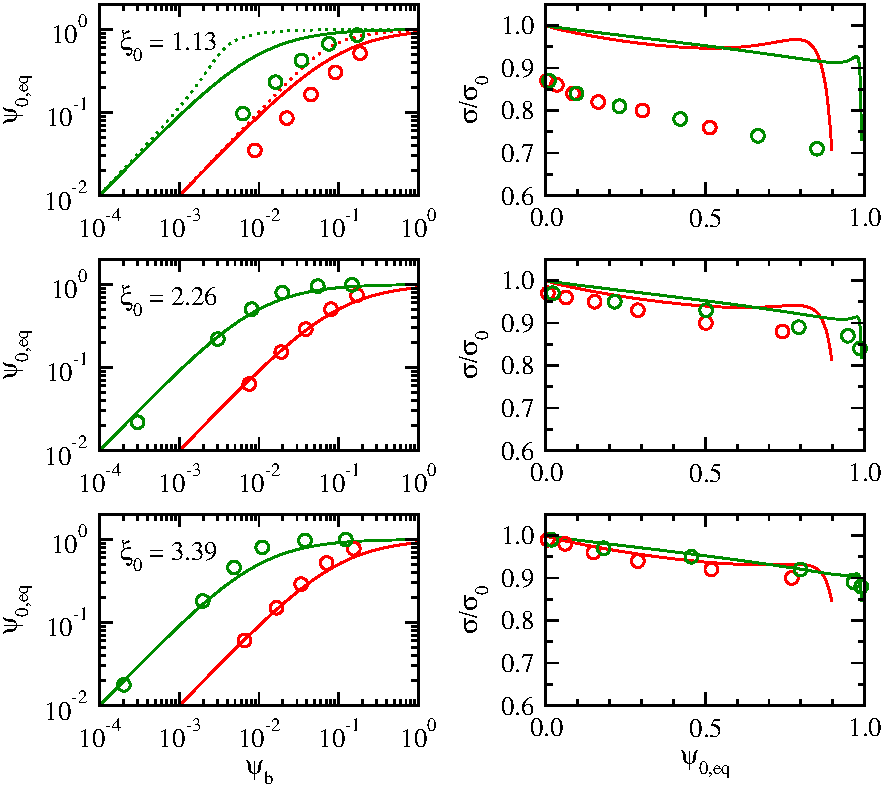
\includegraphics{surfactant_fig1-eps-converted-to.pdf}
\end{center}
\caption{Equilibrium results for one-dimensional simulations with
varying interfacial width $\xi_0$, all other physical parameters
being the same. In particular, $\epsilon = \kappa/4$ and $\beta = 0$.
The
left-hand column shows equilibrium isotherms with $1/K_L$ = 0.1 (red)
and $1/K_L$ = 0.01 (green). The circles are simulations and the lines
the theoretical prediction. The right-hand column shows the
corresponding reduction in surface tension at equilibrium
as a function of $\psi_{0,\mathrm{eq}}$. This reduction is scaled by
the bare interface surface tension $\sigma_0$. The exact result here
is based on a direct numerical integration of the excess free energy
across an equilibrium interfacial profile. The points are computed
by carrying out an analogous numerical integration of the simulated
profile at the given resolution. Note that the representation of
the surfactant porfile is particularly poor at $\xi_0 = 1.13$ as
there turn out to be an even number of lattice points where
$\psi >> \psi_b$ so that the peak value is missed.}
\end{figure}



\subsubsection{Dynamics}

Solve the Ward-Tordai equation.

\subsection{Calibration of the Surface Tension}

The binary fluid model introduces an interfacial tension $\sigma$ which
can be predicted from the choice of free energy \cite{swift,kendon}.
In particular, Kendon et al. 2000 described the process of calibrating
the actual interfacial tension of the model fluid. This was based on
a measurement of the Laplace pressure difference between the fluid
inside and outside a spherical droplet via
\begin{equation}
\Delta p = 2 \sigma / R
\end{equation}
where $R$ is the radius of the spherical drop at equilibrium. This
measurement appears quite difficult in practice owing to tendency of
any initial drop to evaporate \cite{yue2007}.

\subsubsection{New measurement}

Here, we prefer a measure based on the expected profile of the
order parameter $\phi$ and the free energy density at a flat interface.
In order to sample all orientations of the interface with respect to
the lattice we again take a large droplet of fluid A initialised at
rest in fluid B. We assume that the interface is locally flat and so
the procedure holds.

If a droplet with radius $r_0$ is constructed with an initial interfacial
profile of $\phi(r) = \tanh{(r - r_0) / \xi_0}$
with $r$ in the radial direction,  then the free energy density will be
(with $-A = B$)
\begin{equation}
 e(r) = -{\scriptstyle \frac{1}{4}} |A| [1 - \mathrm{sech}^4 (r-r_0)/\xi_0]
+ {\scriptstyle \frac{1}{2}}
 (\kappa/\xi_0^2)\, \mathrm{sech}^4{(r-r_0)/\xi_0}.
\end{equation}
Obtaining a fit to $\xi_0$ from the measured interfacial profile of
$\phi (r)$ and to $ e_0 = \kappa / 2 \xi_0^2$ from the peak in the measured
profile of free energy
density allows an estimate of the interfacial tension to be made:
\begin{equation}
\sigma = 2(8/9)^{1/2} \xi_0 |e_0|.
\end{equation}
This measurement is taken after the initial profile has been allowed
to relax for at least 10 times the larger of the diffusion time
$\xi_0^2 / M$ or the momentum diffusion time $\xi_0^2 / \eta$.


We have measured the surface tension using the following approaches.

\textit{Method 1}.

LB for two distributions with relaxation of order parameter
following Kendon etal. The force on the fluid is applied
via the equilibrium stress following Swift et al.

\textit{Method 2}.

As method 1 but using the realxation of order parameter
following Stratford etal.

\textit{Method 3}.

As Method 1 but with force via divergence of the chemical stress.

\textit{Method 4}.

As Method 3 but with force via divergence of the chemical stress.

\textit{Method 5}.

Using finite difference (1st order upwind) for the order parameter.

\textit{Method 6}.

Using finite difference (3rd order upwind).

\subsubsection{Results}

We follow the parameter sets in Kendon et al Table~2. These
are reproduced here in Table~\ref{tab:r1}. Measured values for
Run028 parameters are show in Table~\ref{tab:newr028}.

\begin{table}
\begin{center}
\begin{tabular}{llllllll}
\hline
Run & $-A, B$ & $\kappa$ & $\eta$ & $M$ & $\sigma$  & $L_0$ & $T_0$ \\
\hline
Rks001 & 0.00625 & 0.004 & 1.41 & 0.05 & 0.0047 & 422 & 1.26e10$^5$\\
Rks002 & 0.00625 & 0.004 & 0.65 & 0.25 & 0.0047 & 89.7 & 1.24e10$^4$\\
Run028 & 0.083 & 0.053 & 1.41 & 0.05  & 0.0625 & 31.8 & 718 \\
Run022 & 0.0625 & 0.04 & 0.5 & 0.25   & 0.0471 & 5.31 & 56.3 \\
Run029 & 0.0625 & 0.04 & 0.2 & 0.15   & 0.0471 & 0.849 & 3.61 \\
Run020 & 0.00625 & 0.004 & 0.025 & 2.00 & 0.00471 & 0.133 & 0.704 \\
Run030 & 0.00625 & 0.004 & 0.0065 & 1.25 & 0.00471 & 0.00829 & 0.0124 \\
Run019 & 0.003125 & 0.002 & 0.0014 & 4.00 & 0.00236 & 0.000831 & 0.000493 \\
Run032 & 0.00125  & 0.0008 & 0.0005 & 5.0 & 0.000943 & 0.000265 & 0.000141\\
\hline  
\end{tabular}
\end{center}
\caption{Table showing common parameter values following Kendon et al.
with the theoretical interfacial tension, $L_0$ and $T_0$. Note that
the order parameter mobility is used here (cf $\tilde{M} = 2M$) in
Kendon et al. (KS values are extra sets used to low 1/$\dot{\gamma}T_0$.)}
\label{tab:r1}
\end{table} 

\begin{table}
\begin{tabular}{lllllll}
\hline
Method & $\xi_0$ & $e_{min}$ & $e_{max}$ & $\sigma$  & $\phi_{min}$
& $\phi_{max}$\\
\hline
\multicolumn{7}{c}{Run028}\\
\hline
Theory   & 1.13 & -0.0207 &  0.0207 & 0.0625 & -1.0 & 1.0 \\
Method 1 & 1.00 & -0.0207 & 0.0128 & 0.063(3) & -1.0091 & 1.0028 \\
Method 2 & 1.00 & -0.0207 & 0.0126 & 0.063(1) & -1.0113 & 0.9993 \\
Method 3 & && & & & \\
Method 4 & && & & & \\
Method 5 & && & & & \\
Method 6 & --& --& --& --& --& --\\
\hline
\multicolumn{7}{c}{Run029}\\
\hline
Theory & 1.13 & -0.0156 & 0.0156 & 0.0471  & -1.0 & 1.0\\
Method 2 & 0.99 & -0.0156 & 0.010(?) & 0.048(4) & -1.0110 & 1.0003\\ 
Method 6 & 1.02 & -0.0156 & 0.0099 & 0.049(0) & -1.0048 & 1.0002\\
\hline
\multicolumn{7}{c}{Run030}\\
\hline
Theory & 1.13 & -0.00156 & 0.00156 & 0.00471 & -1.0 & 1.0\\
Method 2 & 1.04 & -0.00156 & 0.0008(?) & 0.0047(1) & -1.0167 & 1.0063\\
Method 6 & 1.08 & -0.00156 & 0.0007(?) & 0.0048(0) & -1.0028 & 1.0031\\
\hline
\multicolumn{7}{c}{Run019}\\
\hline
Theory & 1.13 & -0.000781 & 0.000781 & 0.00236 & -1.0 & 1.0\\
Method 2 & 1.29(?) & -0.000781 & 0.00015(?) & 0.0022(8) & -1.0312 & 1.0242\\
Method 6 & 1.23(?) & 0.0010(?) &&  0.0024(?) & -1.0085 & 1.0019\\
\hline 
\multicolumn{7}{c}{Run032}\\
\hline
Theory   & 1.13 &  -0.000312 & 0.000312 & 0.000943  & -1.0 &1.0\\
Method 2 & 1.07  & -0.000312& 0.000157 & 0.00094(7) & -1.0511 & 1.0311\\
Method 6 & 1.6(5)& -0.000312 & not st. & 0.0010(7) &-1.0056 & 1.0010\\
\hline
\end{tabular}
\caption{Results for the different methods for Run208 parameters.}
\end{table}

\subsection{User input}

\inputkey{free\_energy surfactant}

Currently under reconstruction.

This is for use with a two order parameter model the first of
which is the composition, as for the symmetric free energy,
while the second $\psi$ represents surfactant concentration.
The free energy density is made up of a number of terms:

\begin{equation}
{\textstyle \frac{1}{2}}A\phi^2
+ {\textstyle \frac{1}{4}}B\phi^4
+ {\textstyle \frac{1}{2}}\kappa (\mathbf{\nabla}\phi)^2
\end{equation}
is the standard symmetric term related to the composition.
These parameters are represented in the input as

\inputkey{surf\_A}
\inputkey{surf\_B}
\inputkey{surf\_kappa}

\begin{equation}
D \left(\psi \ln\psi + (1 - \psi) \ln(1-\psi)\right)
\end{equation}
represents the energy of surfactant in the bulk phase with surfactant
concentration $0 < \psi < 1$ with a single parameter $D$;
\begin{equation}
-{\textstyle \frac{1}{2}} \epsilon \psi (\mathbf{\nabla} \phi)^2
-{\textstyle \frac{1}{2}} \beta \psi^2  (\mathbf{\nabla} \phi)^2
\end{equation}
where the term in $\epsilon$ represents the energy reduction by
adsorbing surfactant at the interface and the term in $\beta$
provides an additional favourable term modelling the fact that
the molecules like to line up; finally, there is an extra term
\begin{equation}
+{\textstyle \frac{1}{2}} W \psi \phi^2
\end{equation}
which is included to stabilise the interface \cite{theissengompper}.

The corresponding keys for the input file are:

\inputkey{D} is the bulk surfactant contribution parameter

\inputkey{epsilon} is the parameter $\epsilon$

\inputkey{W} is the parameter $W$

\inputkey{beta} is the value of the parameter $\beta$.

\inputkey{phi\_b} the initial, uniform, background surfactant
concentration $\psi_b$.

\inputkey{mobility\_psi} Sets the (uniform) mobility for the surfactant
as appropriate for the Cahn-Hilliard equation.



\vfill
\pagebreak


\clearpage
\vfill\pagebreak
\section{Electrokinetics}

\subsection{Sress tensor in the electrosymmetic model}

\subsubsection{Definitions}

The total free energy functional is a function of the composition $\phi$, the density of the ionic species $\rho_\alpha$,

\beq
{\cal F}[\phi,\{\rho_\alpha\}] = \int d{\bf r} \;F\left(\phi({\bf r}),\{\rho_\alpha({\bf r})\}\right). 
\eeq

The free energy density can be factorised into a contribution from the composition and an ionic contribution according to

\beqa
F&=&F^{mix} +F^{ion}\\
F^{mix}&=& \frac{1}{2} \,A \,\phi^2 + \frac{1}{4} \,B \,\phi^4+ \frac{1}{2} \kappa(\bm{\nabla}\phi)^2\\
F^{ion,ex}&=& \sum_{\alpha=\pm} \rho_\alpha \left(V^{solv}_\alpha-\mu_\alpha +\frac{z_\alpha e}{2}\Psi \right).
\eeqa

In the ionic contribution we have omitted the ideal gas contribution of the ions.
The solvation energy is given by

\beqa
V^{solv}_\alpha({\bf r})=\Delta\mu_\alpha\frac{1+\phi({\bf r})}{2}
\eeqa

It is convenient to define the total free energy without electric field $F_0$, i.e. with vanishing electric potential:  

\beqa
F_0&=&F^{mix} +F^{ion,ex}|_{\Psi=0}
\eeqa

The Poisson equation reads
\beqa
\bm{\nabla}\left(\varepsilon({\bf r})\bm{\nabla}\Psi({\bf r})\right)=-\sum_{\alpha=\pm} e \,z_\alpha \,\rho_\alpha ({\bf r})
\eeqa

whereas the electric field is given by

\beq
{\bm E}=-{\bm \nabla}\Psi.
\eeq

The permittivity depends on the composition $\phi$ via

\beqa
\varepsilon({\bf r})=\bar{\varepsilon} \,(1-\gamma\,\phi({\bf r}))
\eeqa

The electric displacement field 

\beq
{\bm D}({\bf r})=\varepsilon({\bf r}){\bm E}({\bf r})
\eeq

The 'co-energy' density 

\beq
\tilde{F}=F_0-\frac{\varepsilon}{2}\bm{E}^2
\eeq

has the meaning of a Legendre transform of the free energy density $F_0$.

\subsubsection{Electromechanical stress tensor}

The electromechanical stress tensor is generally defined as \cite{Landau-ED, Melcher}. 

\beqa
\sigma_{i j}=\varepsilon E_i E_j + \delta_{i j}\left( \tilde{F} - \phi \frac{\delta \tilde{\cal F}}{\delta\phi} - \sum_{\alpha=\pm} \rho_\alpha \frac{\delta \tilde{\cal F}}{\delta\rho_\alpha}\right).
\eeqa

The first functional derivative yields

\beqa
\phi \frac{\delta\tilde{\cal F}}{\delta\phi}&=&\phi\left(\frac{\delta {\cal F}_0}{\delta\phi}-\frac{{\bm E}^2}{2} \frac{\partial \varepsilon}{\partial\phi}\right)\\
&=&\phi\left(\frac{\partial F_0}{\partial\phi}-{\bm \nabla}\left(\frac{\partial F_0}{\partial {\bm \nabla}\phi}\right)-\frac{{\bm E}^2}{2} \frac{\partial \varepsilon}{\partial\phi}\right)\\
&=&A\,\phi^2+B\,\phi^4-\kappa\phi({\bm \nabla}^2\phi)+\frac{\phi}{2}\sum_{\alpha=\pm} \rho_\alpha \Delta\mu_\alpha+\phi\,\frac{\bar{\varepsilon}\gamma}{2}{\bm E}^2\\
&=&A\,\phi^2+B\,\phi^4-\kappa\phi({\bm \nabla}^2\phi)+\frac{\phi}{2}\sum_{\alpha=\pm} \rho_\alpha \Delta\mu_\alpha-\frac{\varepsilon-\bar{\varepsilon}}{2}{\bm E}^2,
\eeqa

where we used the above dependence of the permittivity on the composition.
The second functional derivative is given by 

\beqa
\rho_\alpha \frac{\delta \tilde{\cal F}}{\delta\rho_\alpha}&=&\rho_\alpha\left(\frac{\delta {\cal F}_0}{\delta\rho_\alpha}\right)\\
&=&\rho_\alpha(V^{solv}_\alpha-\mu_\alpha)
\eeqa

The co-energy density and the functional derivatives with respect to composition $\phi$ and ionic densities $\rho_\alpha$ add up to 

\beqa
\tilde{F} - \phi \frac{\delta \tilde{F}}{\delta\phi} - \sum_{\alpha=\pm} \rho_\alpha \frac{\delta \tilde{F}}{\delta\rho_\alpha}=&&\nonumber\\
&&\hspace*{-4cm}=-\frac{\varepsilon}{2}\bm{E}^2+\frac{A}{2} \phi^2 + \frac{B}{4} \phi^4+ \frac{\kappa}{2} (\bm{\nabla}\phi)^2 \nonumber\\
&&\hspace*{-3cm}-A\phi^2-B\phi^4+ \kappa\phi({\bm \nabla}^2\phi) -\frac{\phi}{2}\sum_{\alpha=\pm} \rho_\alpha \Delta\mu_\alpha\nonumber\\
&&\hspace*{-3cm}-\phi\,\frac{\bar{\varepsilon}\gamma}{2}{\bm E}^2-\sum_{\alpha=\pm}\rho_\alpha(V^{solv}_\alpha-\mu_\alpha)\\
&&\hspace*{-4cm}=-\frac{\varepsilon}{2}\bm{E}^2-\frac{A}{2}\phi^2 -\frac{3 B}{4} \phi^4+ \frac{\kappa}{2}(\bm{\nabla}\phi)^2 + \kappa\phi({\bm \nabla}^2\phi) \nonumber\\
&&\hspace*{-3cm}-\frac{\phi}{2}\sum_{\alpha=\pm} \rho_\alpha \Delta\mu_\alpha -\phi\,\frac{\bar{\varepsilon}\gamma}{2}{\bm E}^2
\eeqa

This yields

\beqa
\sigma_{ij}&=&\varepsilon E_i E_j - \delta_{i j}\left(\frac{\varepsilon}{2}\bm{E}^2+\frac{A}{2}\phi^2 +\frac{3\,B}{4}\phi^4 - \frac{\kappa}{2} (\bm{\nabla}\phi)^2\right.\nonumber\\
&&\left.- \kappa\phi({\bm \nabla}^2\phi) +\frac{\phi}{2}\sum_{\alpha=\pm} \rho_\alpha \Delta\mu_\alpha +\phi\,\frac{\bar{\varepsilon}\gamma}{2}{\bm E}^2\right).\nonumber\\
\eeqa

In order to satisfy the condition of mechanical equilibrium $\nabla_j \sigma_{ij}=0$ a symmetric contribution has to be added to the above stress tensor. The following lines try to elucidate this.\\

Taking the divergence of the stress tensor gives

\beqa
\nabla_j\sigma_{i j}&=& (\nabla_j \varepsilon E_j) E_i + \varepsilon E_j \nabla_j E_i + \nabla_i\left( \tilde{F} - \phi \frac{\delta \tilde{\cal F}}{\delta\phi} - \sum_{\alpha=\pm} \rho_\alpha \frac{\delta \tilde{\cal F}}{\delta\rho_\alpha}\right)\\
&=& \left({\bm \nabla}\cdot{\bm D}\right) E_i+ D_j \nabla_j E_i +\nabla_i F_0 - D_j \nabla_i E_j \nonumber\\
&&\hspace*{0.5cm} -\nabla_i\left(\phi \frac{\delta \tilde{\cal F}}{\delta\phi} +\sum_{\alpha=\pm} \rho_\alpha \frac{\delta \tilde{\cal F}}{\delta\rho_\alpha}\right)\\
&=& \left({\bm \nabla}\cdot{\bm D}\right) E_i + D_j \left(\nabla_j E_i-\nabla_i E_j\right) + \nabla_i F_0\nonumber\\
&&\hspace*{0.5cm} -\nabla_i\left(\phi \mu_\phi +\sum_{\alpha=\pm} \rho_\alpha \mu_{\rho_\alpha}\right)
\eeqa

According to Gauss' law the first term is 

\beq
\left({\bm \nabla}\cdot{\bm D}\right)E_i = \rho_f E_i=\sum_{\alpha=\pm} z_\alpha e \rho_\alpha E_i,
\eeq
 
whereas $\rho_f$ is the free charge density.
Moreover, due to Faraday's law the curl in the second bracket vanishes.
This leads us to the following intermediate result: 

\beqa
\nabla_j\sigma_{i j}&=& \sum_{\alpha=\pm}z_\alpha e \rho_\alpha E_i + \nabla_i F_0 - \nabla_i\left(\phi \mu_\phi +\sum_{\alpha=\pm} \rho_\alpha \mu_{\rho_\alpha}\right)\\
&=&\sum_{\alpha=\pm} z_\alpha e \rho_\alpha E_i + \frac{\partial F_0}{\partial \phi} \nabla_i \phi + \frac{\partial F_0}{\partial \nabla_j \phi} \nabla_j \nabla_i \phi +\sum_{\alpha=\pm} \left\{\frac{\partial F_0}{\partial \rho_\alpha}\right\} \nabla_i \rho_\alpha\nonumber\\
&&\hspace*{0.5cm} -\nabla_i\left(\phi \mu_\phi +\sum_{\alpha=\pm} \rho_\alpha \mu_{\rho_\alpha}\right)\\
&=& \sum_{\alpha=\pm} z_\alpha e \rho_\alpha E_i + \left\{\frac{\partial F_0}{\partial \phi} - \nabla_j \left(\frac{\partial F_0}{\partial \nabla_j \phi}\right)\right\} \nabla_i \phi +\nabla_j\left(\frac{\partial F_0}{\partial \nabla_j \phi} \nabla_i \phi\right)\nonumber\\
&&\hspace*{0.5cm} +\sum_{\alpha=\pm} \left\{\frac{\partial F_0}{\partial \rho_\alpha} \right\}\nabla_i \rho_\alpha-\nabla_i\left(\phi \mu_\phi +\sum_{\alpha=\pm} \rho_\alpha \mu_{\rho_\alpha}\right).
\eeqa

If we replace the terms in curly brackets the chemical potentials $\mu_\phi$ and $\mu_{\rho_\alpha}$ and use the fact that gradients of the chemical potential vanish in equilibrium, we end up with

\beqa
\nabla_j\sigma_{i j}&=& \sum_{\alpha=\pm}z_\alpha e \rho_\alpha E_i + \nabla_j\left(\frac{\partial F_0}{\partial \nabla_j \phi} \nabla_i \phi\right)
\eeqa

The first term is the external force on the charges, which is zero if we have no counterions and an equal amount of positve and negative ions. Therefore, we have to add a term 

\beq
-\left(\frac{\partial F_0}{\partial \nabla_j \phi} \nabla_i \phi\right)
\eeq

to the stress tensor to fulfill the equilibrium condition. This is equivalent to similar derivations in \cite{Landau-EL}.\\

The total stress tensor reads

\beqa
\sigma_{ij}&=&\varepsilon E_i E_j - \kappa (\nabla_i\phi)(\nabla_j\phi)  - \delta_{i j}\left(\frac{\varepsilon}{2}\bm{E}^2+\frac{A}{2}\phi^2 +\frac{3\,B}{4}\phi^4\right.\nonumber\\
&&\left. - \frac{\kappa}{2} (\bm{\nabla}\phi)^2- \kappa\phi({\bm \nabla}^2\phi) +\frac{\phi}{2}\sum_{\alpha=\pm} \rho_\alpha \Delta\mu_\alpha +\phi\,\frac{\bar{\varepsilon}\gamma}{2}{\bm E}^2\right).
\eeqa

\subsection{Examples}

A number of regression tests 
verify the implemention of the Nernst-Planck equation in 
combination with the SOR solver. They can be found in

\begin{verbatim}
trunk/tests/regression
\end{verbatim}

The original tests we carried out during the first
implementation comprise the Gouy-Chapman theory
for electric double layers in front of a charged wall \cite{Lyklema},
the liquid junction potential emerging between two electrolytes
of slighty different concentration and diffusivity of the charged species \cite{Mafe},
electro-osmotic flow in a slit pore  \cite{Capuani, Rotenberg} 
and Debye-H\"uckel theory for charged 
colloidal particles and small enough potentials \cite{Lyklema}.
They are described in the following paragraphs.


\subsubsection{Gouy-Chapman}

This validation test is a flat surface carrying a surface charge $\sigma$
with counterions and symmetic electrolyte. This is a one-dimensional, 
electroneutral problem of a diffusive electric double layer which has 
an analytical solution \cite{Lyklema}. 
The approximation for low electrostatic 
potentials reads

\begin{figure}[htpb]
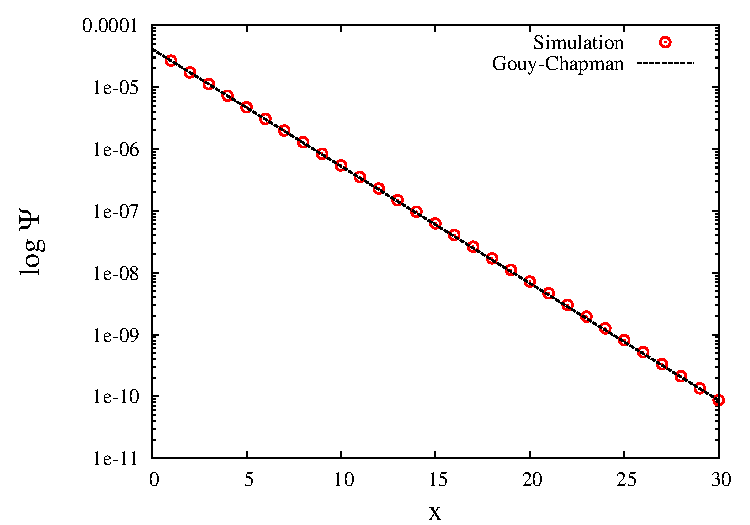
\includegraphics[width=0.495\textwidth]{./pics/test1.pdf}
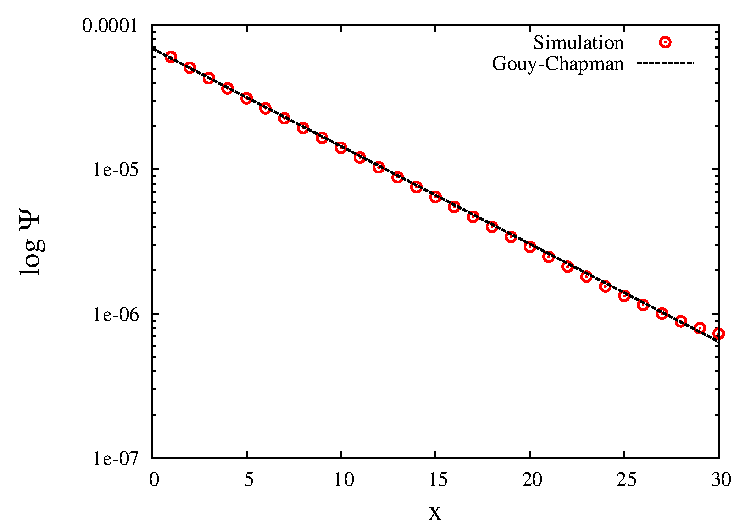
\includegraphics[width=0.495\textwidth]{./pics/test2.pdf}
\caption{Gouy-Chapman theory for electric double layers: The plots compare the simulation results for the electric potential with the analytical solution for $\rho_{0,\pm}=1\e{-2}$ (left) and $\rho_{0,\pm}=1\e{-3}$ (right).} 
\label{fig1} 
\end{figure}


\begin{equation}\label{gouychapman}
\Psi(x) = \Psi_D \exp(-\kappa\, x)
\end{equation}
with $\kappa$ as inverse Debye length 
\begin{equation}
\kappa = l_D^{-1} = \sqrt{8\pi\, l_B \, I}.
\end{equation}
The Bjerrum length $l_B$ is given by 
\begin{equation}
l_B = \frac{\beta\,e^2}{4\pi\,\varepsilon}
\end{equation} 

with $\beta^{-1}=k_B T$, $e$ as unit charge and $\varepsilon=\varepsilon_0\varepsilon_r$ 
as dielectric permittivity.
The parameter 

\begin{equation}
I = \frac{1}{2}\sum_k z_k^2\; \rho_{B,k}
\end{equation} 

is the ionic strength 
of the electrolyte with $z_k$ as valencies of species $k$
($z_\pm=\pm 1$ for simple symmetric electrolyte) and $\rho_{B,k}$ as 
bulk charge density of species $k$ far away from the wall.
The Stern potential $\Psi_D$ at the surface of the wall is related 
to the surface charge $\sigma$ via

\begin{eqnarray}
\Psi_D&=&\frac{2}{\beta \,e} \sinh^{-1}\left(-\sigma\,p\right)\\
\Psi_D&\simeq&\frac{2}{\beta \,e} \ln\left(-\sigma \, p + \sqrt{(\sigma\,p)^2+1}\right)\\
p &=& \frac{1}{\sqrt{8\, \varepsilon\, \beta^{-1} \,\rho_B}}.
\end{eqnarray}

The quantity $\rho_B=\rho_{B,+}=\rho_{B,-}$ is 
the average bulk charge density of the electrolyte.

We solved the Gouy-Chapman problem for a 
system consisting of $L_x \times L_y \times L_z=64\times4\times4$
lattice sites. Periodic boundary conditions were used at all sides 
and a no-flux boundary conditions was set at $L_x=1$ and $L_x=64$.

\begin{figure}[htpb]
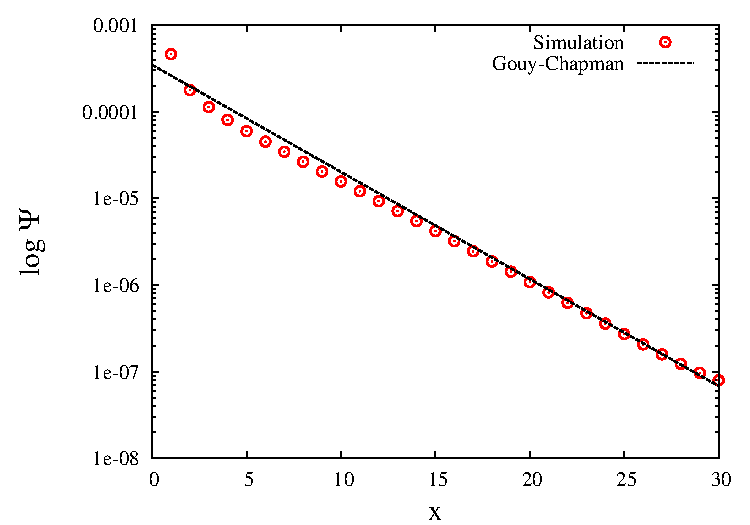
\includegraphics[width=0.495\textwidth]{./pics/test3.pdf}
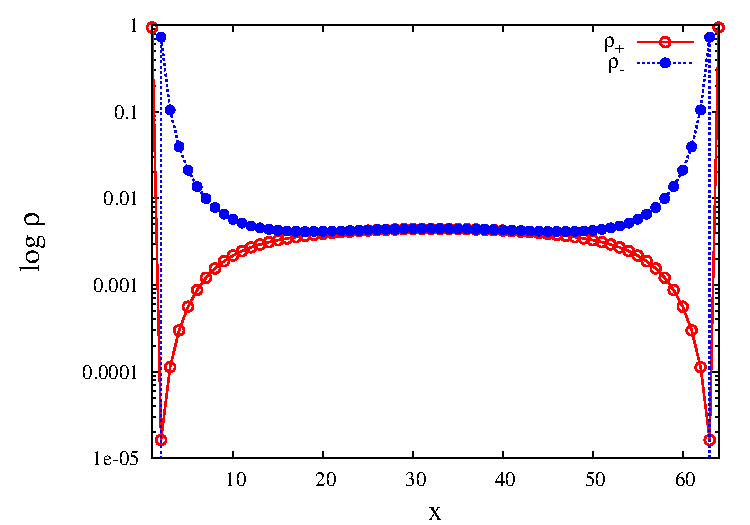
\includegraphics[width=0.495\textwidth]{./pics/test3-rho.pdf}
\caption{Nonlinear regime: For larger surface charges the solution deviates from the low-potential approximation Eq. \ref{gouychapman} to the Gouy-Chapman theory. The righthand picture shows the charge distribution across the gap.} 
\label{fig2} 
\end{figure}

 
The parameters were chosen as follows (all in simulation units):
unit charge $e=1$, temperature $k_B T=\beta^{-1}=3.333\e{-5}$, valency $z_{\pm}=\pm1$, 
dielectric permittivity $\varepsilon=3.3\e{3}$, diffusivities 
of the species $D_{\pm}=1\e{-2}$ and initial densities $\rho_{0,\pm}=1\e{-2}$.
The entire system was electro-neutral and had a Bjerrum length $l_B=0.723$.

At first we tested the linear case applying a small positive surface charge
$\sigma=3.125\e{-2}$, which led to bulk charge density $\rho_{B,+}=\rho_{B,-}=1.044\e{-2}$, 
Debye length $l_D=2.295$ and surface potential $\Psi_D=2.136\e{-5}$.
The potential was initialised with zero and had a value $\Psi_c=-2.364\e{-6}$ 
in the centre of the system after equilibration which we subtracted in the 
following analysis.

We reduced the initial density of the electrolyte to $\rho_{0,\pm}=1\e{-3}$,
which resulted in bulk charge densities  
$\rho_{B,+}=1.298\e{-3}, \rho_{B,-}=1.370\e{-3}$, 
Debye length $l_D=6.420$, surface potential $\Psi_D=5.451\e{-5}$
and centre potential $\Psi_c=-1.256\e{-5}$.
The comparison with the approximate solution Eq. \ref{gouychapman} is shown 
in Fig. \ref{fig1}.

For larger surface charges the low-potential assumption which led to Eq. \ref{gouychapman}
is no longer valid and the nonlinear nature of the Poisson-Boltzmann 
equation becomes evident.
Fig. \ref{fig2} shows the results for a surface charge $\sigma=9.375\e{-1}$
and electrolyte density $\rho_{0,\pm}=3\e{-3}$. We obtained for   
bulk charge densities $\rho_{B,+}=4.443\e{-3}$ and $\rho_{B,-}=4.461\e{-3}$, 
Debye length $l_D=3.514$, the surface potential $\Psi_D=2.267\e{-4}$
and the centre potential $\Psi_c=-3.395\e{-5}$. 

\subsubsection{Liquid-junction potential}

The liquid junction potential 
is a charge separation process that 
occurs when electrolytes with slightly different concentrations
whose species have different diffusivities are brought into contact.
Charges from the regions of higher concentration diffuse   
into the parts with lower concentration. Due to the difference 
in diffusivity they migrate at different speeds, leaving parts of
the system charged. This leads to a build-up of a potential
which balances the diffusive flux.

After the initial build-up phase the potential decreases slowly 
again until the charge concentration has become homogeneous throughout 
the system. Both timescales of emergence and decay of the potential
can be separated by chosing a sufficiently large system size.

This problem allowed us to verify the correct temporal 
behaviour of the Nernst-Planck equation solver by resolving the transient 
dynamics without having to account for advective terms.

\begin{figure}[h!t]
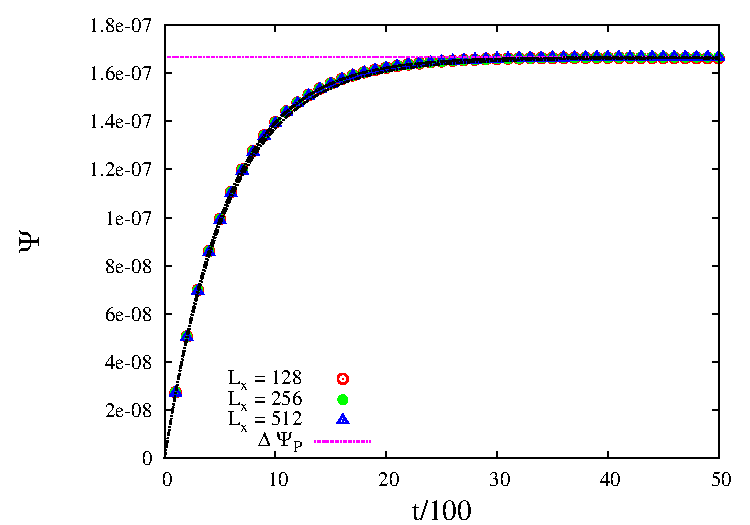
\includegraphics[width=0.495\textwidth]{./pics/test_lj_zoom1.pdf}
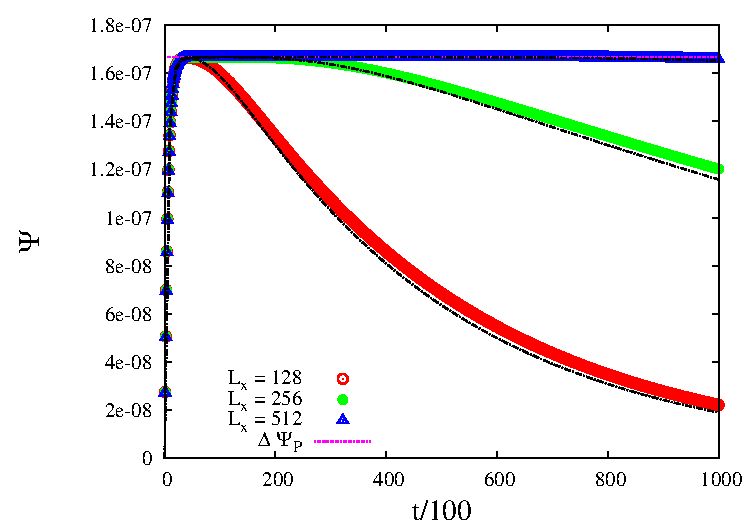
\includegraphics[width=0.495\textwidth]{./pics/test_lj_zoom3.pdf}
\caption{Time evolution of the liquid junction potential for $L_x=128$ (blue), $L_x=256$ (green) and $L_x=512$ (blue). The dashed black curves represent the approximate solution in the limit $l_D/L_x<<1$. Deviations can be seen which are presumably due
to the approximate nature of the analytical solution and the fact that we
have a different asymptotic flux close to the boundary - the theoretical 
analysis assumes no flux at a boundary which is infinitely far away from
the diffusive region.} 
\label{fig3} 
\end{figure}

For simplicity we considered systems of size 
$L_x\times L_y\times Lz=128\times4\times4$ and 
$L_x\times L_y\times Lz=256\times4\times4$ with
periodic boundary conditions at either end.
The two halfs were electroneutral and had ionic concentrations 
$\rho_{L,\pm}=\rho_{0,\pm} + \delta\rho$ and 
$\rho_{R,\pm}=\rho_{0,\pm} - \delta\rho$ 
with $\rho_{0,\pm}=1\e{-2}$ and $\delta\rho = 0.01$.

The potential difference between both sides during the build-up 
obeys approximately

\begin{equation}
\Delta\Psi(t)\simeq\Delta\Psi_P \left\{1-\exp\left(-\frac{t}{\tau_e}\right)\right\}\\
\end{equation}

with 

\begin{equation}
\Delta\Psi_P=\frac{(D_+ D_-)}{\beta e (D_+ + D_-)} \frac{\delta\rho}{\rho_0}\\ 
\end{equation}

as saturation value of the potential difference.
The saturation time scale is given by

\begin{equation}
\tau_e=\frac{\varepsilon}{\beta \, e^2 (D_+ + D_-) \rho_0}.
\end{equation}

\begin{figure}[htpb]
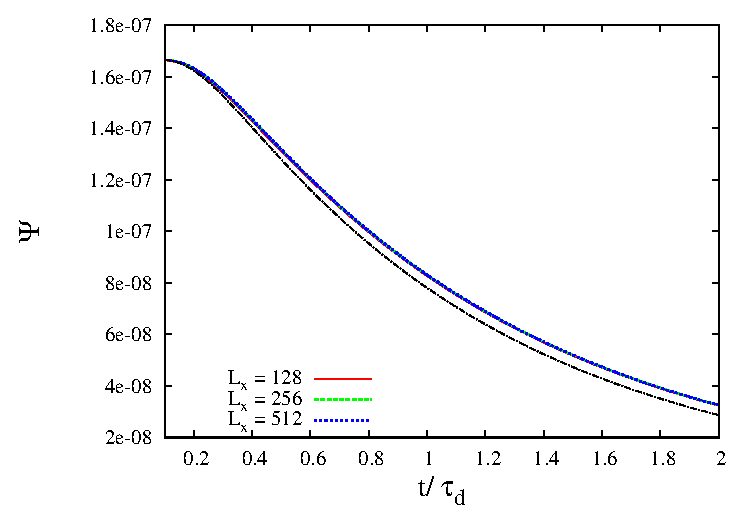
\includegraphics[width=0.9\textwidth]{./pics/test_lj_decay1.pdf}
\caption{Rescaled plot of the decay: Times have been Time evolution of the liquid junction potential for $L_x=128$ (blue), $L_x=256$ (green) and $L_x=512$ (blue). The dashed black curves represent the approximate solution in the limit $l_D/L_x<<1$. Deviations can be seen which are due
to the approximate nature of the analytical solution and the diffusive fluxes close to the boundary.} 
\label{fig4} 
\end{figure}

A more exact solution can be derived in the limit $l_D/L_x<<1, N\to\infty$: 
 
\begin{eqnarray}
\Delta\Psi(t)&=&\Delta\Psi_P \left\{1-\exp\left(-\frac{t}{\tau_e}\right)\right\}\frac{4}{\pi}\left\{\sum_{m=1}^N \frac{\sin^3(m\pi/2)}{m} \exp\left(-\frac{ m^2\, t}{\tau_d}\right)\right\}\\
\tau_d&=&\frac{L^2}{2\pi^2 (D_+ + D_-)}.\label{taud}
\end{eqnarray}

It contains as well the dependence on the decay timescale $\tau_d$.
Only odd indices $m$ contribute to the sum:
 
\begin{eqnarray}
\sum_{m=1}^N \frac{\sin^3(m\pi/2)}{m} \exp\left(-\frac{m^2\, t}{\tau_d}\right)&=&\nonumber\\
&&\hspace*{-4cm} \exp\left(-\frac{t}{\tau_d}\right)-\frac{1}{3} \exp\left(-\frac{9 t}{\tau_d}\right)+\frac{1}{5}\exp\left(-\frac{25t}{\tau_d}\right)-\frac{1}{9}\exp\left(-\frac{81 t}{\tau_d}\right)+\ldots
\end{eqnarray}

A complete discussion of the solution can be found in \cite{Mafe}. 
There, the upper limit of significant modes has been also estimated as $N_{max} = L/\pi l_D$.
Note the factor 2 difference between Eq. \ref{taud} and the corresponding expression in \cite{Mafe}.

The following parameters were used:
dielectric permittivity $\epsilon=3.3\e{3}$, temperature $\beta^{-1}=3.333\e{-5}$, unit charge $e=1$, valency $z_\pm=\pm1$, diffusivities $D_+=0.0125$ and $D_-=0.0075$.
We obtained
$\Delta\Psi_P=1.6667\e{-7}$, $\tau_e=550$, $\tau_d=41501.2\, (L_x=128)$, $\tau_d=166004.6\, (L_x=256)$ and $\tau_d=664018.5 (L_x=512)$.
The results for the potential difference over time are shown in Fig. \ref{fig3}.

Fig. \ref{fig4} shows results with times rescaled to the decay 
time scale $\tau_d$ (cf. Eq. \ref{taud}). Obviously the 
deviations we observe are not due to the limited system size 
and have a more systematic origin. 

The curves coincide if 
the theoretic limit for $\tau_d$ is rescaled by a factor $1.067$,
suggesting the effective system length for this sort of setup is
actually about 3\% larger than the numerical value.

A reason for this might be the approximate nature of the analytical solution 
and the fact that it was gained
for an infinitely large system with constant charge concentrations,
vanishing currents at both ends and finite diffusive zone of size $L_x$.
In our situation the entire system is within the diffusive zone.
This may lead to smaller effective diffusivities or larger effective
system sizes.
Interestingly, all runs with solid walls at both ends resulted in 
oscillatory behaviour and an effective system size of $2L_x$.


\subsubsection{Electroosmotic Flow}

To test the implementation with all couplings to external and 
internal forces we consider a forced charged fluid in a slit
of size $L_z$. An electrostatic field $E_{||}$ is allied
parallel to the walls. The entire system is electroneutral with 
each wall having the surface charge density $\sigma$ 
and compensationg counterions with total charge $2 \sigma A_{wall}$
in the fluid.

In equilibrium the charge density at a distance $x$ from the wall obeys

\begin{equation}
\rho(x)=\frac{\rho_0}{\cos^2(K\,x)}
\end{equation}

with 

\begin{equation}
\rho_0=K^2/2\pi l_B
\end{equation}

and 

\begin{eqnarray}
K \,L_x \tan\left(\frac{K\, L_x}{2}\right)&=&\pi\, l_B\, L_x\, 2\sigma\label{kex} \\
K \,L_x&\simeq&\sqrt{4\pi \,l_B\,L_x\,2\sigma}\label{klin}.
\end{eqnarray}


The liniarised version Eq. \ref{klin} has only a limited range of applicabilty.
We solved Eq. \ref{kex} numerically and found solutions 
$K=0.01959\; (\sigma=0.003125)$ and $K=0.03311\; (\sigma=0.00125)$, 
which is reasonably far away from the 
theoretical limit $K_{max}=\pi/L_x$ set by the tangent. 

Note the factor 2 difference on the lhs of Eq. \ref{kex} with respect 
to \cite{Capuani, Rotenberg}. There is also a factor $L_x$ missing on 
the rhs of Eq. \ref{klin}.

The steady state velocity of the fluid can be derived from the 
force balance of the gradient of the stresses and the electrostatic
forces:

\begin{eqnarray}
v_y(x)&=&\hat{v} \ln\left(\frac{\cos(K\,x)}{\cos(K\,L_x/2)}\right)\label{vy}\\
\hat{v}&=&\frac{e \,E_{||}\rho_o}{\eta\, K^2}=\frac{e \,E_{||}}{2\pi\eta l_B}\label{vhat}
\end{eqnarray}

The result for two different charge densities is shown in Fig. \ref{fig6}.
The accuracy is acceptable with deviations for high surface 
charged potentially being caused by the chosen discretisation or 
by the numerical solution of Eq. \ref{kex} approaching the limit 
of $\pi/L_z\simeq0.049$.  

\begin{figure}[htpb]
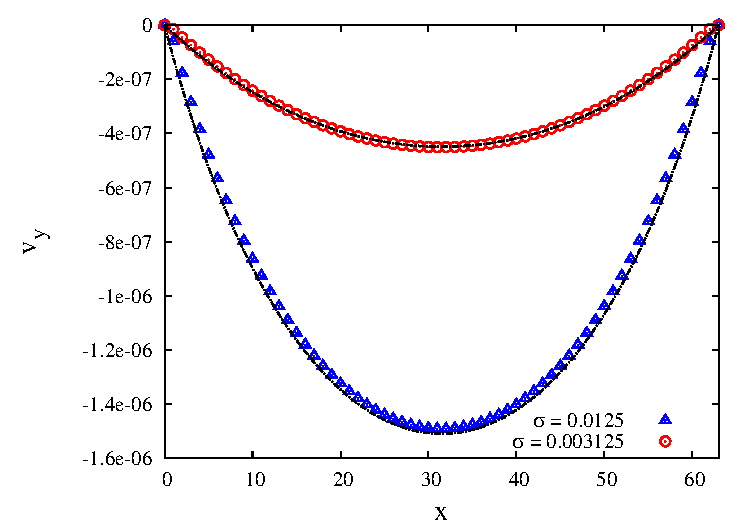
\includegraphics[width=0.9\textwidth]{./pics/test_eo.pdf}
\caption{Steady state flow profile across a slit of width $L_x=63$ for an applied field of magnitude $e \beta E L_x=1.89$ for two different charge densities $\sigma=0.003125$ (red) and $\sigma=0.0125$ (blue), Bjerrum length $l_B=0.7234$, viscosity $\eta=0.1$ and unit charge $e=1$. The dashed black lines correspond to theoretical prediction according to Eqs. \ref{vy} and \ref{vhat}.} 
\label{fig6} 
\end{figure}

\subsubsection{Debye-H\"uckel Theory}

We have tested the implementation for a single fixed
colloid and compared the result with Debye-H\"uckel theory. A result
is shown in Fig.~\ref{fig7}.
We used the following parametrisation:

$L_x \times L_y \times L_z=64\times64\times64$,
$D_+=D_-=0.01$,
$e=1$, 
$z_{\pm}=1$,
$\beta^{-1}=3.333\e{-5}$,
$\varepsilon=3.3\e{3}$,
$l_B=0.723$.

For a central and fixed colloid of radius $R_c=7.5$ carrying a positive unit charge
$q_{c,+}=1.0, q_{c,-}=0$ we obtained 
$\rho_{c,+}=5.58\e{-4}$,
$\rho_{el}=\rho_{B,\pm}=1\e{-2}$, 
$\Psi_D=8.836\e{-7}$ for $2\,R_c=16$.

For a higher larger positive charge $q_{c,+}=4.0$ we got
$\rho_{c,+}=2.23\e{-3}$
$\rho_{el}=\rho_{B,\pm}=5\e{-3}$ 
$\Psi_D=4.993\e{-6}$ for $2\,R_c=16$.

\begin{figure}[htpb]
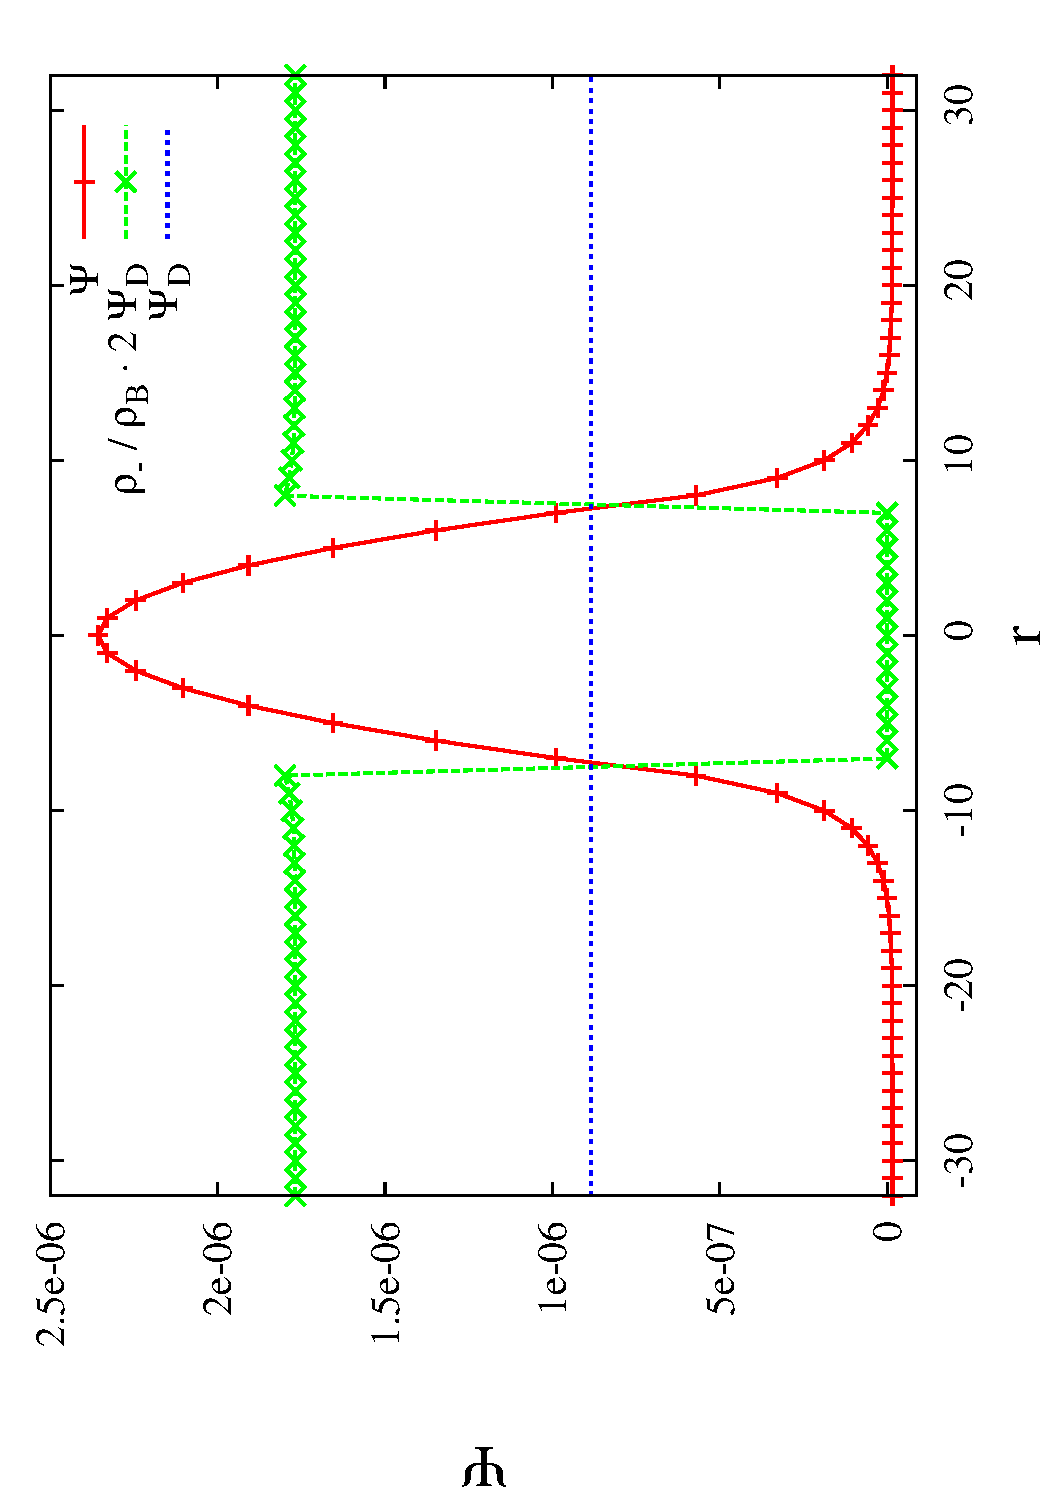
\includegraphics[angle=-90,width=0.9\textwidth]{./pics/test_dh1.pdf}\\
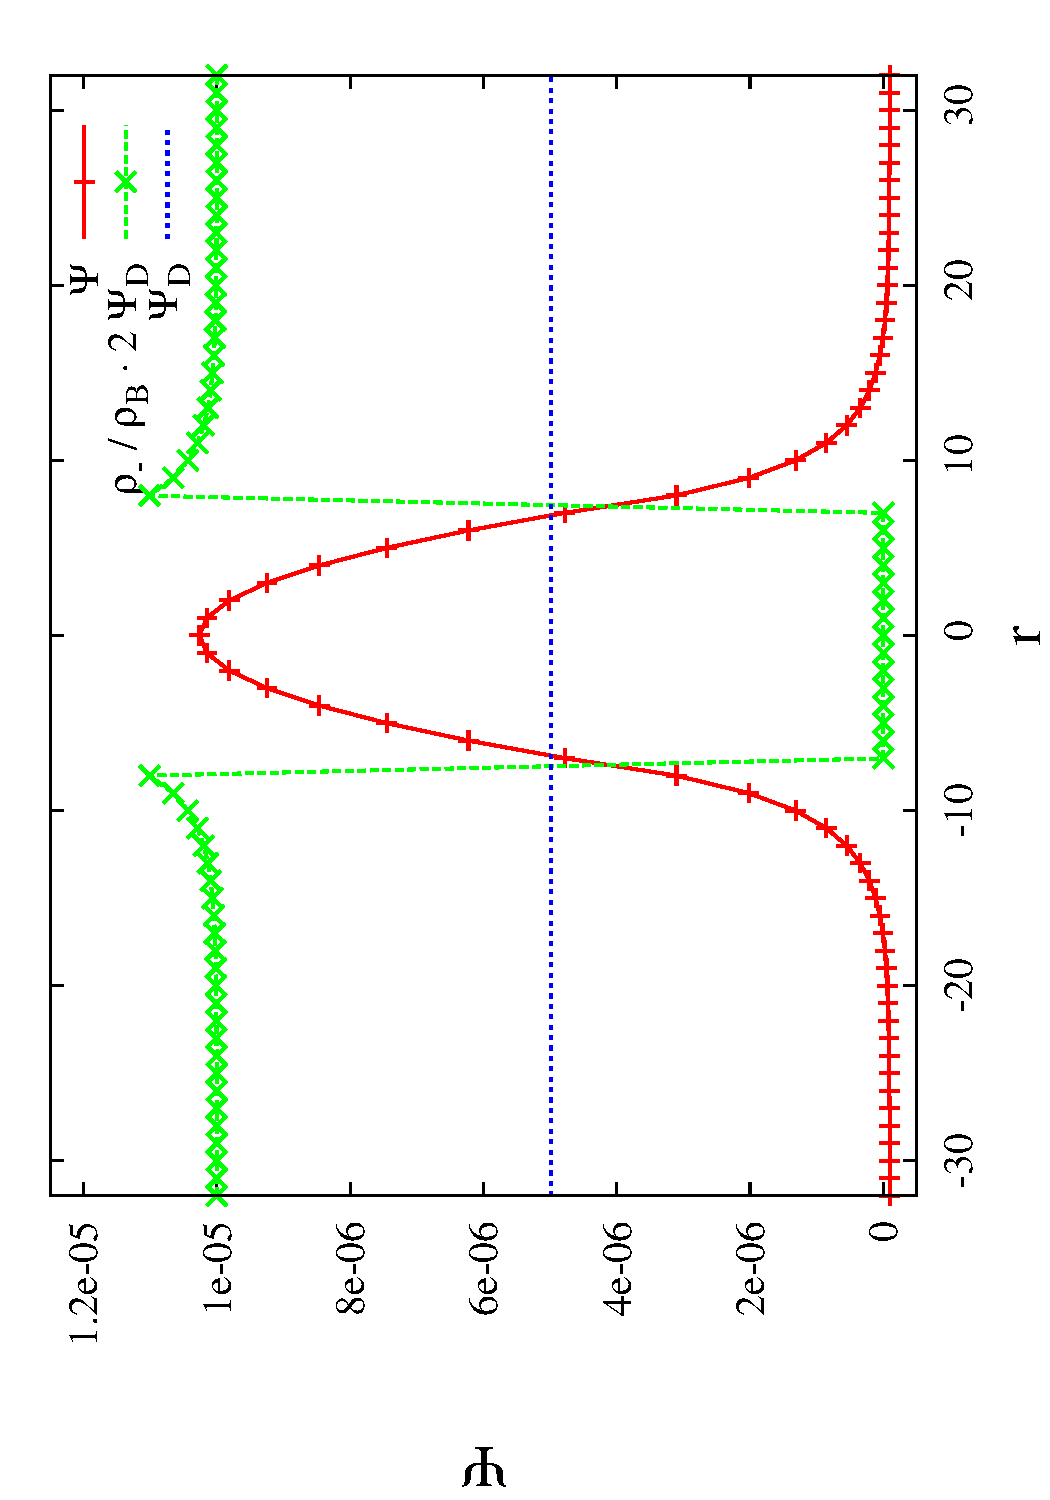
\includegraphics[angle=-90,width=0.9\textwidth]{./pics/test_dh2.pdf}
\caption{Debye-H\"uckel theory for positively charged colloid: the picture
shows a cut through the center of a single colloid in a peridoic system.
The potential is shown in red, the Stern potential in blue, and the negative 
charge density in green. The colloid is in the center.}
\label{fig7}
\end{figure}
\clearpage

\subsubsection{Scaling of the SOR}

We have run some simple scaling tests for the electrokinetic problem
with zero fluid velocity. A system of $128^3$ lattice sites was used
as representative of a small production system. The code was run on
the Mare Nostrum machine in Barcelona for a small number of time
steps to assess performance on up to 512 MPI tasks. The results are
shown in Fig. \ref{fig5}. 

While the scaling for the Nernst Planck part of
the calulcation are reasonable, it can be seen that the SOR routine
used to solve the Poisson equation is not really acceptable. This
was not unexpected. Some improvements might be possible, but the
algorithm is essentailly unsuitable for large systems. 

\begin{figure}[htpb]
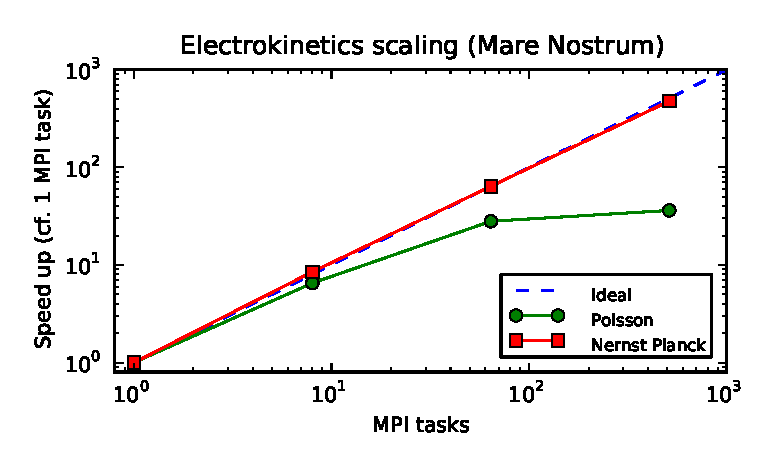
\includegraphics[width=0.9\textwidth]{./pics/scaling.pdf}
\caption{Scaling of a system of $128^3$ lattice sites on up to 512 MPI tasks. 
While the scaling for the Nernst Planck part of the calulcation are reasonable, 
it can be seen that the SOR routine used to solve the Poisson equation deviates
strongly from ideal behaviour.} 
\label{fig5} 
\end{figure}

\subsubsection{Scaling with Krylov Subspace Solver}

We use a Krylov subspace solver from the Portable Extendabl Toolkit for Scientific Computation (PETSc. 

\begin{figure}[htpb]
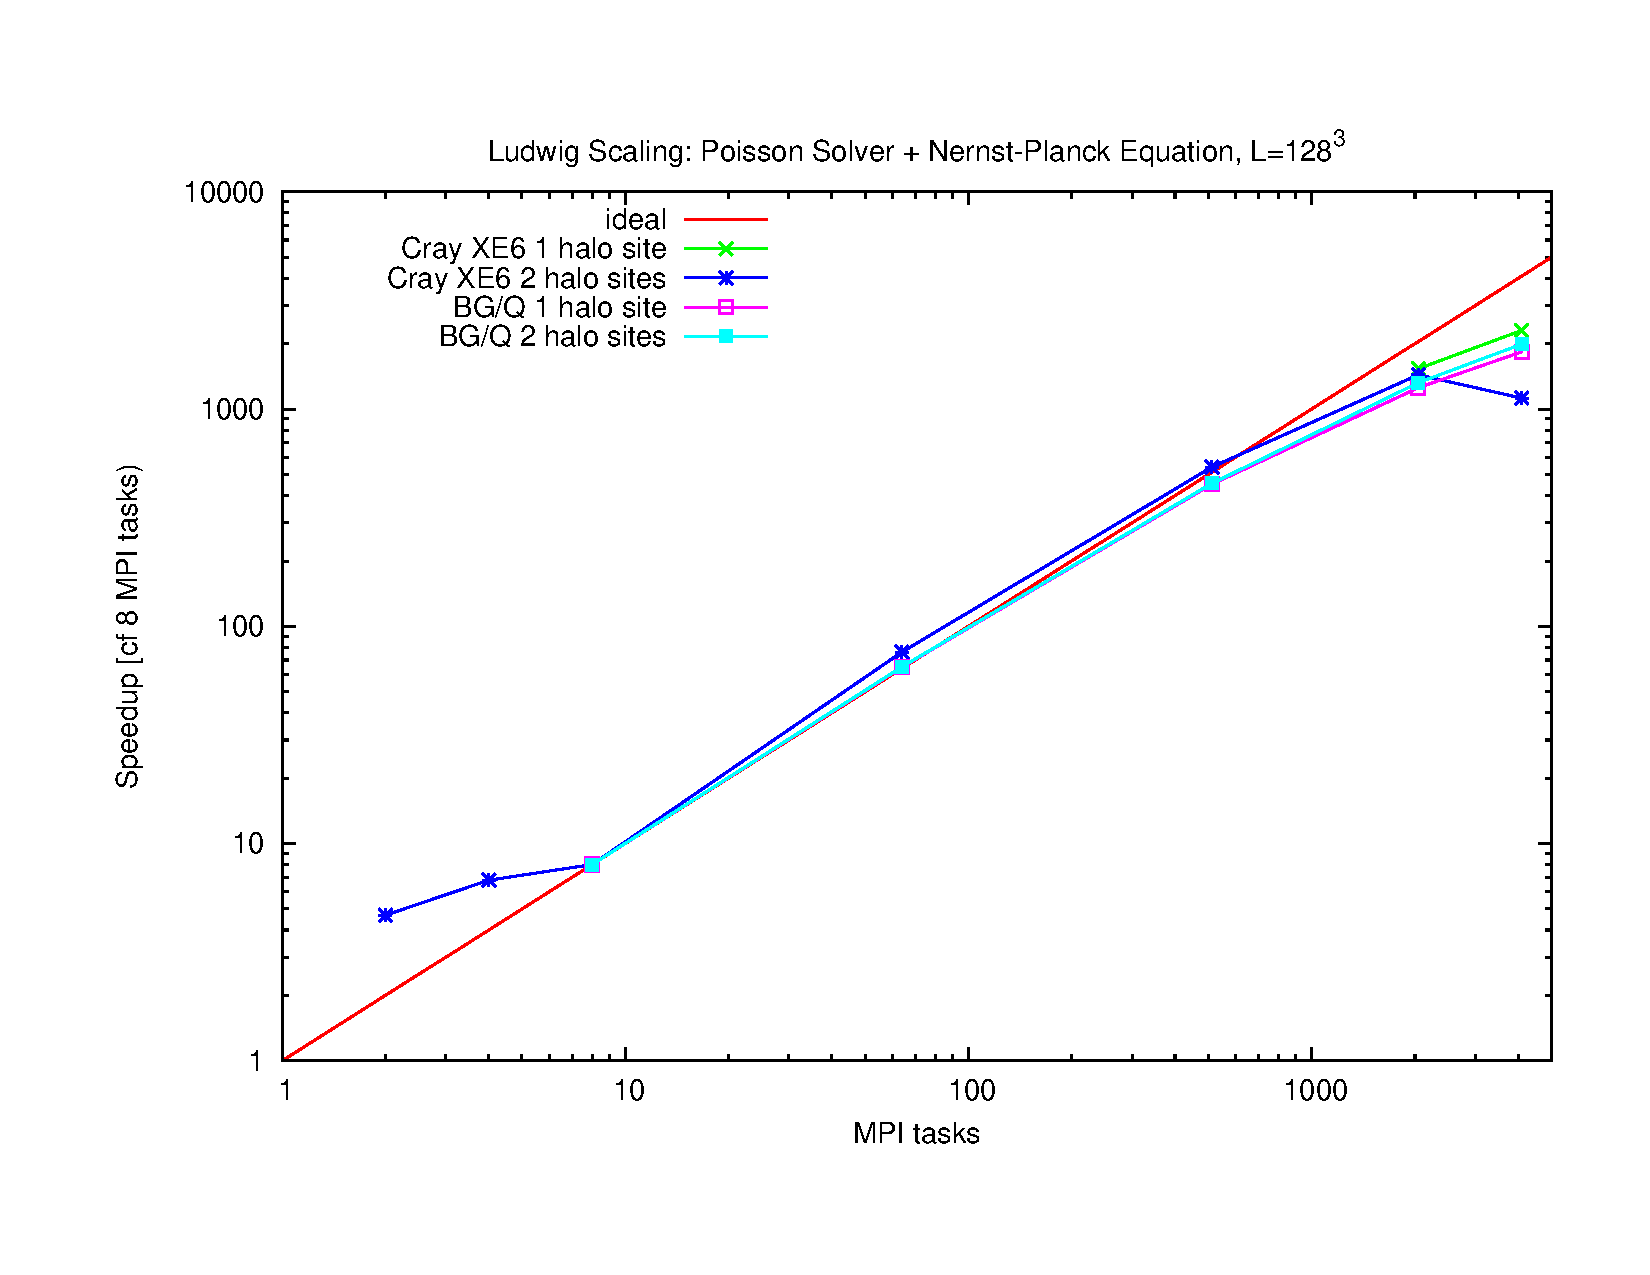
\includegraphics[width=0.9\textwidth]{./pics/petsc_scaling.pdf}
\caption{Scaling of a system of $128^3$ lattice sites on up to 4096 MPI tasks. 
The scaling of both the Nernst Planck part as well as the Poisson solver are only limited by the overhead of communication to computation at very small decompositions.} 
\label{fig6} 
\end{figure}
\clearpage


\subsection{User input}


%\clearpage
%\vfill\pagebreak
%%%%%%%%%%%%%%%%%%%%%%%%%%%%%%%%%%%%%%%%%%%%%%%%%%%%%%%%%%%%%%%%%%%%%%%%%%%%%%
%
%  plan.tex
%
%  Software Configuration Management Plan
%
%  Edinburgh Soft Matter and Statistical Physics Group and
%  Edinburgh Parallel Computing Centre
%
%  Kevin Stratford (kevin@epcc.ed.ac.uk)
%  (c) 2011-2015 The University of Edinburgh
%
%%%%%%%%%%%%%%%%%%%%%%%%%%%%%%%%%%%%%%%%%%%%%%%%%%%%%%%%%%%%%%%%%%%%%%%%%%%%%


\section{Software Configuration Management Plan}

\subsection{Introduction}

\subsubsection{Purpose}

This section contains information on the \textit{Software Configuration
Management Plan} for the \textit{Ludwig} code.
It is to provide users of the code a background on the way in which
the code is developed, how bugs are dealt with, the way in which
new features may be added, how correctness is ensured and tested, and so on.
It is therefore a part
of the process by which the code is maintained. The Software Configuration
Management Plan will be referred to as `The Plan' throughout the remainder
of the section.

\subsubsection{Scope}

The \textit{Ludwig} code is designed to study the hydrodynamic properties
of simple and complex fluids based around the numerical solution of the
Navier-Stokes equations. Complex fluids are dealt with via a free-energy
based finite difference approach, which couples explicitly to the
hydrodynamics.
Components of \textit{Ludwig} include the main program, unit and
regression tests, and a small number support libraries, and a small
number of utility programs used to prepare
input and post-process output. The Plan is limited to these
software components.

\textit{Ludwig} is specifically designed for parallel computers and
relies on the Message Passing Interface \cite{mpi-standard}. The
code will also run in serial, and is independent of
the platform it is run on. The Plan is not concerned with
hardware or system management activities.

\textit{Ludwig} is an on-going research project, and relies mainly
on funding for the United Kingdom Engineering and Physical Sciences Research
Council to provide support for staff time to work on maintenance and
development.

% IEEE section to be completed
%\subsubsection{Definition of key terms}

\subsubsection{References}

This section is based on the IEEE standard for Software Configuration
Management Plans IEEE 828-2012 \cite{ieee-828-2012}, and follows the format
set out therein.
Relevant references are included and can be found in the main References
section at the end of the document.

\subsection{Management}

\subsubsection{Organisations}

\textit{Ludwig} is developed by a team based in the School of Physics at
The University of Edinburgh. This involves two groups: the Soft Matter
Physics Group, and Edinburgh Parallel Computing Centre (EPCC). These
groups collaborate with a number of workers at different Universities
around the world on different aspects of the code.

\subsubsection{Responsibilities}

While the Soft Matter Physics Group is responsible for the overall
scientific direction and development of the code and concomitant
priorities, all the Software Configuration Management activities will
be the responsibility of EPCC.

% IEEE section recheck what this actually means
% \subsubsection{Procedures}
% There are currently no external constraints on The Plan.

\subsubsection{Process Management}

EPCC is responsible for the Software Configuration Management process.
It is anticipated that the cost of this process will be small as the
project team can communicate informally on a regular basis. There is
currently no independent
surveillance of activities to ensure compliance with The Plan.

\subsection{Activities}

\subsubsection{Identification}

The material under control of the project includes three sets of files:
this documentation, the source code, and the test suite which is used
to monitor the status of the code.
Control of project files is via a single on-line repository which
uses the subversion (SVN) revision control system. The SVN repository
is currently located at

\texttt{http://ccpforge.cse.rl.ac.uk/}

which is maintained at the Rutherford Appleton Laboratory on behalf
of Collaborative Computational Physics 5 (The Computer Simulation of
Condensed Phases). Subversion identifies different revisions by a
unique revision number. A given version of a file is then uniquely
identified by its path in the repository as it exists at a given
revision number.

% Add pointer to standard manifest (README)

All access to the code is via the CCPForge repository. CCPForge identifies
three different levels of access:

\textit{Administrators:} allows administration of the site itself and
registered members;

\textit{Developers:} members who have write access to the source code repository;

\textit{Users:} have read only access to the source code via SVN (either
as a member or via anonymous download). Member users also have access to
the tracker.

As CCPForge is not physically under the control of EPCC, a
complete dump of the repository to a local resource is undertaken on a
regular basis for security.

\subsubsection{Control}

Requests for changes or additions to the code should be made via
the issue tracker at CCPForge. The project team will then decide
whether the change is possible and/or desirable. If so, the
implementation and testing of the change will take place, and the
new code committed back to the repository.

\textit{Submitting a change request:} A description of the proposed change
will be submitted to the CCPForge issue tracker as a change request to
provide a record of the change process.

\textit{Evaluating a change request:} The request, together with any
additional information, will be evaluated by the SCM team. The request
will be accepted, refined, or rejected as appropriate. The change owner
will make necessary updates to the change record.

\textit{Implementation of change:} Important changes to behaviour of code
related to a change will be
accompanied by a relevant descriptive record in the change request.

\textit{Version control:} A \texttt{MAJOR.MINOR.PATCH} numerical version
name scheme is used \cite{apacheAPR}.
It is expected that bug fixes and relatively
small changes will be accompanied by a unit increment in the patch level;
more significant changes will be reflected at the minor version number;
major reconstructions will occur rarely and incur a change of major version
number.

\subsubsection{Status}

% Privides tracability of changes, pending completed, etc
% Configuration reports, release notes

The status of changes will be tracked at the CCPForge issue tracker
with a named SCM team member owning the change. The relevant tracker
item will be closed when successfully implemented and tested.

The tracker is available to CPPForge member users to provide a record
of changes to the code. Anonymous users will be alerted to changes via
release notes.

%\subsubsection{Evaluation and review}
%There are currently no formal mechna audit the code?

% \subsubsection{Interface control}
% This section discusses other organisations the developers must
% ``interface'' with.

% IEEE section not relevant
%\subsubsection{Subcontractor / vendor control}


\subsubsection{Release management and delivery}

There are currently no formal releases of the \textit{Ludwig} code.
Any release management and  delivery will be via the SVN repository.


% IEEE section. We don't really have any schedules.
%\subsection{Schedules}

%\subsection{Resources}

% Software resources (dependencies, etc)
% Hardware resources
% Human resources

\subsection{Plan Maintenance}

The Plan is currently under review to consider organisational changes
affecting the responsibilities different stakeholders.



%\begin{thebibliography}{99}

%Software Configuration Management Plans''
%\bibitem{mpi-standard} Message Passing Interface Forum. MPI: A Message
%Passing Interface Standard Version 1.3 (1998).
%\bibitem{paraview} Paraview is a standard visualisation package. 


\clearpage
\vfill\pagebreak
%%%%%%%%%%%%%%%%%%%%%%%%%%%%%%%%%%%%%%%%%%%%%%%%%%%%%%%%%%%%%%%%%%%%%%%%%%%
%
%  references.tex
%
%  Bibliography
%
%  $Id$
%
%  Edinburgh Soft Matter and Statistical Physics Group and
%  Edinburgh Parallel Computing Centre
%
%  Kevin Stratford (kevin@epcc.ed.ac.uk)
%  (c) 2011 The University of Edinburgh
%
%%%%%%%%%%%%%%%%%%%%%%%%%%%%%%%%%%%%%%%%%%%%%%%%%%%%%%%%%%%%%%%%%%%%%%%%%%%

\vfill
\pagebreak

\addcontentsline{toc}{section}{References}

\bibliographystyle{plain}
\begin{thebibliography}{99}

\bibitem{adhikari_desplat}
Adhikari, R. J.-C. Desplat, and K. Stratford,
Sliding periodic boundary conditions for lattice Boltzmann and lattice
kinetic equations,
\texttt{arXiv:cond-mat/0503175v1} (2005).

\bibitem{adhikari2005}
Adhikari, R., K. Stratford. M.E. Cates, and A.J. Wagner,
Fluctuating Lattice Boltzmann,
\textit{Europhys. Lett.}, \textbf{71}, 473 2005.

\bibitem{ald98}
Aidun, C.K., Y. Lu, and E.-J. Ding,
Direct analysis of particulate suspensions with inertia using the
discrete Boltzmann equation,
\textit{J. Fluid Mech.}, \textbf{373}, 287, 1998.

\bibitem{batchelor}
G.K. Batchelor
\textit{An Introduction to Fluid Mechanics},
Cambridge University Press (1967).

\bibitem{blake}
J.R. Blake, A spherical envelope approach to ciliary propusion,
\textit{J. Fluid Mech.}, \textbf{46}, 199, 1971.

\bibitem{cates_scaling}
M. E. Cates, J.-C. Desplat, P. Stansell, A.J. Wagner, K. Stratford,
R. Adhikari, and I. Pagonabarraga,
Physical and Computational Scaling Issues in Lattice Boltzmann
Simulations of Binary Fluid Mixtures,
\textit{Phil. Trans. Roy. Soc. A}, \textbf{363}, 1917 (2005). 

\bibitem{chunladd}
B. Chun and A.J.C. Ladd,
Interpolated boundary condition for lattice Boltzmann simulations in
narrow gaps,
\textit{Phys. Rev. E}, \textbf{75}, 066705, 2007.

\bibitem{cj98}
Cichocki, B., and R.B. Jones,
Image representation of a spherical particle near a hard wall,
\textit{Physica A}, \textbf{258}, 273, 1998.

\bibitem{chang}
C.-H. Chang and E.I. Franses,
Adsorption dynamics of surfactants at the air/water interface:
a critical review of mathematical models, data, and mechanisms,
\textit{Colloids and Surfaces A}, \textbf{100} 1, 1995.

\bibitem{cpc}
Desplat, J.-C., I. Pagonabarraga, and P. Bladon,
LUDWIG: A parallel lattice-Boltzmann code for complex fluids.
\textit{Comput. Phys. Comms.}, \textbf{134}, 273, 2001.

\bibitem{diamant}
H. Diamant and D. Andelman,
Kinetics of surfactant adsorption at fluid/fluid
interfaces: non-ionic surfactants,
\textit{Europhys. Lett.} \textbf{34}, 575 (1996).

\bibitem{diamant96}
H. Diamant and D. Andelman,
Kinetics of surfactant adsorption at fluid-fluid interfaces,
\textit{J. Phys. Chem.}, \textbf{100} 13732, 1996.

\bibitem{fournier2005}
J.-B. Fournier and P. Galatola,
Modeling planar degenerate wetting and anchoring in nematic liquid
crystals,
\textit{Europhys. Lett.}, \textbf{72} 403--409 (2005).

\bibitem{eastoe}
J. Eastoe and J.S. Dalton,
Dynamic surface tension and adsorption mechanims of surfactants
at the air-water interface,
\textit{Advances in Colloid and Interface Science}, \textbf{85}
13, 2000.

\bibitem{ginzburg}
I. Ginzburg and D. d'Humi\`eres,
Multireflection boundary conditions for lattice Boltzmann models,
\textit{Phys. Rev. E}, \textbf{68}, 066614, 2003.

\bibitem{h59}
Hasimoto, H., On the periodic fundamental solutions of the Stokes
equation and their application to viscous flow past a cubic array
of spheres.
\textit{J. Fluid Mech.}, \textbf{5}, 317.

\bibitem{heemels}
Heemels, M.W., M.H.J. Hagen, and C.P. Lowe, Simulating solid colloidal
particles using the lattice-Boltzmann method,
\textit{J. Comp. Phys.}, \textbf{164}, 48, 2000.

\bibitem{ieee-208}
IEEE Standard 208-2005, IEEE Standard for Software Configuration Management
Plans. See \texttt{http://ieeexplore.ieee.org/xpl/standards.jsp}
(accessed 2011).

\bibitem{jo84}
Jeffrey, D.J., and Y. Onishi,
Calculation of the resistance and mobility functions for the two
unequal rigid spheres in low-Reynolds-number flow,
\textit{J. Fluid Mech.}, \textbf{139}, 261, 1984.

\bibitem{viv}
Kendon, V.M., M.E. Cates, I. Pagonabarraga, J.-C. Desplat, and
P. Bladon,
Inertial effects in three dimensional spinodal decomposition of
a symmetric binary fluid mixture: A lattice Boltzmann study,
\textit{J. Fluid Mech.}, \textbf{440}, 147 (2001).

\bibitem{l94a}
Ladd, A.J.C., Numerical simulations of particulate suspensions
via a discretised Boltzmann equation. Part 1. Theoretical foundation,
\textit{J. Fluid. Mech.}, \textbf{271}, 285, 1994.

\bibitem{l94b}
Ladd, A.J.C., Numerical simulations of particulate suspensions
via a discretised Boltzmann equation. Part 2. Numerical results,
\textit{J. Fluid. Mech.}, \textbf{271}, 311, 1994.

\bibitem{l96a}
Ladd, A.J.C., Sedimentation of homogenous suspensions of non-Brownian
spheres,
\textit{Phys. Fluids}, \textbf{9}, 491. 1996.

\bibitem{l96b}
Ladd, A.J.C., Hydrodynamic screening in sedimentating suspensions
of non-Brownian spheres,
\textit{Phys. Rev. Lett.}, \textbf{76}, 1392, 1996.

\bibitem{lv01}
Ladd, A.J.C., and R. Verberg,
Lattice-Boltzmann simulations of particle-fluid suspensions,
\textit{J. Stat. Phys.}, \textbf{104}, 1191, 2001.

\bibitem{lipanmiller}
H. Li, C. Pan, and C.T. Miller,
Pore-scale investigation of viscous coupling effects for two-phase
flow in porous media,
\textit{Phys. Rev. E}, \textbf{72}, 026705, 2005.

\bibitem{lighthill}
M.J. Lighthill,
On the squirming motion of nearly spherical deformable bodies through
liquid at very small Reynolds numbers,
\textit{Comm. Pure Appl. Math.}, \textbf{5}, 109, 1952.

\bibitem{isaac}
I. Llopis Fust\'e,
\textit{Hydrodynamic cooperativity in micro-swimmer suspensions},
Ph.D. Thesis, University of Barcelona, 2008.

\bibitem{mpi-standard}
Message Passing Interface Forum. MPI: A Message Passing Interface Standard
Version 1.3 (2008).

\bibitem{nguyen-ladd2002}
Nguyen, N.-Q., and A.J.C. Ladd, Lubrication corrections for
lattice-Boltzmann simulations of particle suspensions,
\textit{Phys. Rev. E}, \textbf{66}, 046708, 2002.

\bibitem{papanastasiou}
T. paapnastasiou, G. Georgiou, and A. Alexandrou,
\textit{Viscous Fluid Flow},
CRC Press, Boca Raton, Florida, 2000.

\bibitem{paraview}
Paraview. See \texttt{http://www.paraview.org/}. Accessed 2011.

\bibitem{r95}
Rapaport, D.C., \textit{The Art of Molecular Dynamics Simulation},
Cambridge University Press, 1995.

\bibitem{succi}
S. Succi, \textit{The lattice Boltzmann equation and beyond},
Oxford University Press, Oxford, 2001.

\bibitem{edo1}
M. Venuroli and E.S. Boek,
Two-dimensional lattice-Boltzmann simulations of single phase
flow in a pseudo two-dimensional micromodel,
\textit{Physica A}, \textbf{362}, 23, 2006.

\bibitem{vandergraaf}
R.G.M. van der Sman and S. van der Graaf,
Diffuse interface model of surfactant adsorption onto flat and
droplet interfaces,
\textit{Rheol. Acta} \textbf{46} 3 (2006).

\bibitem{theissengompper}
O. Theissen and G. Gompper,
Lattice Boltzmann study of spontaneous emulsification,
\textit{Eur. Phys. J. B}, \textbf{11} 91 (1999).

\bibitem{wardtordai}
A.F.H. Ward and L. Tordai,
\textit{J. Chem. Phys.} \textbf{14} 453, 1946.

\bibitem{skarabot}
M. Skarabot, M. Ravnik, S. Zumer, U. Tkalec, I. Poberaj, D. Babic, N. Osterman and I. Musevic,
\textit{Phys. Rev. E} \textbf{76}, 051406 (2007).

\bibitem{wright}
D.C. Wright and N.D. Mermin,
\textit{Rev. Mod. Phys.} \textbf{61}, 385 (1989).

\bibitem{Lyklema} J. Lyklema {\em Fundamentals of Interface and Colloid Science} Academic Press     (1995).
\bibitem{Mafe} S. Maf\'e, J.A. Manzanares, J. Pellicer, {\textit J. Electroanal. Chem.} {\textbf 241}, 5    7-77 (1988).
\bibitem{Capuani} F. Capuani, I. Pagonabarraga, D. Frenkel, {\textit J. Chem. Phys.} {\textbf 121}, 973-    986 (2004).
\bibitem{Rotenberg} B. Rotenberg, I. Pagonabarraga, D. Frenkel, {\textit Farad. Discuss.} {\textbf 144},     223-243 (2010).
\bibitem{Landau-ED} L.D. Landau, E.M. Lifshitz, {\textit Electrodynamics of Continuous Media}, \S 15    , 2nd ed., Pergamon Press, Oxford, UK (1984).
\bibitem{Melcher} J.R. Melcher, {\textit Continuum Electromechanics}, \S 3.10, MIT Press, Cambridge,     MA, USA (1981).\\
downloadable from:\\
\url{http://ocw.mit.edu/ans7870/resources/melcher/resized/cem_811.pdf}
\bibitem{Landau-EL} L.D. Landau, E.M. Lifshitz, {\textit Theory of Elasticity}, \S 3 \& \S 16, 3rd e    d., Butterworth-Heinemann, Oxford, UK (1986).



\end{thebibliography}




\end{document}
